\documentclass[a4paper,12pt]{article}[abntex2]
\bibliographystyle{abntex2-alf}


% Definições de layout e formatação
\usepackage{amsmath,amssymb,mathtools}
\usepackage{physics}   % \dv, \pdv, \expval, etc.
\usepackage{bm} 
\usepackage{mathrsfs}
\usepackage[scr=rsfs,cal=boondox]{mathalfa}
\usepackage[a4paper, left=3.0cm, top=3.0cm, bottom=2.0cm, right=2.0cm]{geometry} % Personalização das margens do documento
\usepackage{setspace} % Controle do espaçamento entre linhas
\onehalfspacing % Espaçamento entre linhas de 1,5
\usepackage{indentfirst} % Indentação do primeiro parágrafo das seções
\usepackage{newtxtext} % Substitui a fonte padrão pela Times Roman
\usepackage{titlesec} % Personalização dos títulos de seções
\usepackage{ragged2e} % Melhor controle de justificação do texto
\usepackage[portuguese]{babel} % Adaptação para o português (nomes e hifenização)
\usepackage{amsmath}

% Pacotes de cabeçalho, rodapé e títulos
\usepackage{fancyhdr} % Customização de cabeçalhos e rodapés
\setlength{\headheight}{14.49998pt} % Altura do cabeçalho
\pagestyle{fancy}
\fancyhf{} % Limpa cabeçalho e rodapé
\rhead{\thepage} % Página no canto direito do cabeçalho

% Pacotes para tabelas
\usepackage{booktabs} % Melhora a qualidade das tabelas
\usepackage{tabularx} % Permite tabelas com larguras de colunas ajustáveis
\usepackage{float} % Melhor controle sobre o posicionamento de figuras e tabelas

% Pacotes para gráficos e imagens
\usepackage{graphicx} % Suporte para inclusão de imagens

\usepackage[utf8]{inputenc}
\usepackage{listingsutf8}

\lstset{
    language=R,                      
    basicstyle=\ttfamily\scalefont{1.0},
    keywordstyle=\color{blue},       
    stringstyle=\color{red},         
    commentstyle=\color{green},      
    numbers=left,                    
    numberstyle=\tiny\color{gray},   
    stepnumber=1,                    
    numbersep=5pt,                   
    backgroundcolor=\color{lightgray!10}, 
    frame=single,                    
    breaklines=true,                 
    captionpos=b,                    
    keepspaces=true,                 
    showspaces=false,                
    showstringspaces=false,          
    showtabs=false,                  
    tabsize=2,
     literate={á}{{\'a}}1
             {é}{{\'e}}1
             {í}{{\'i}}1
             {ó}{{\'o}}1
             {ú}{{\'u}}1
             {Ú}{{\'U}}1
             {â}{{\^a}}1
             {ê}{{\^e}}1
             {î}{{\^i}}1
             {ô}{{\^o}}1
             {û}{{\^u}}1
             {ã}{{\~a}}1
             {õ}{{\~o}}1
             {ç}{{\c{c}}}1,
}


% Pacotes para unidades e formatação numérica
\usepackage{siunitx} % Tipografia de unidades do Sistema Internacional e formatação de números
\sisetup{
  output-decimal-marker = {,},
  inter-unit-product = \ensuremath{{}\cdot{}},
  per-mode = symbol
}
\DeclareSIUnit{\real}{R\$}
\newcommand{\real}[1]{R\$#1}

% Pacotes para hiperlinks e referências
\usepackage{hyperref} % Suporte a hiperlinks
\usepackage{footnotehyper} % Notas de rodapé clicáveis em combinação com hyperref
\hypersetup{
    colorlinks=true,
    linkcolor=black,
    filecolor=magenta,      
    urlcolor=cyan,
    citecolor=black,        
    pdfborder={0 0 0},
}
\makeatletter
\def\@pdfborder{0 0 0} % Remove a borda dos links
\def\@pdfborderstyle{/S/U/W 1} % Estilo da borda dos links
\makeatother

% Pacotes para texto e outros
\usepackage{lipsum} % Geração de texto dummy 'Lorem Ipsum'
\usepackage[normalem]{ulem} % Permite o uso de diferentes tipos de sublinhados sem alterar o \emph{}

\begin{document}

\begin{titlepage}
    \centering
    \vspace*{1cm}
    \Large\textbf{INSPER – INSTITUTO DE ENSINO E PESQUISA}\\
    \Large ECONOMIA\\
    \vspace{1.5cm}
    \Large\textbf{Caderno}\\
    \textbf{Desenvolvimento Econômico}\\
    \vspace{1.5cm}
    Prof. Eduardo Correio de Souza, \href{mailto:eduardocs@insper.edu.br}{eduardocs@insper.edu.br} \\
    Prof. Auxiliar  \\
    \vfill
    \normalsize
    Hicham Munir Tayfour, \href{mailto:hichamt@al.insper.edu.br}{hichamt@al.insper.edu.br}\\

    \vfill
    São Paulo\\
    Fevereiro/2025
\end{titlepage}

\newpage
\tableofcontents
\thispagestyle{empty} % Esse comando remove a numeração de pagina da tabela de conteúdo

\newpage 
\listoffigures
\thispagestyle{empty} % Esse comando remove a numeração de pagina da tabela de figura

\newpage
\setcounter{page}{1} % Inicia a contagem de páginas a partir desta página
\justify
\onehalfspacing


\section*{\textbf{Programa do Curso}}

\textbf{Horários Importantes}

As \textit{aulas} acontecem às segundas e quartas-feiras, ambas das 13h30 às 15h30 para a turma A, enquanto para a turma B, também ocorrem nas segundas e quartas-feiras das 15h45 às 17h45 para a turma B. 

Os \textit{horários de atendimento} acontecem as 14h30 às 16h00 nas terças-feiras(de forma presencial, na sala 708) e também nas quintas-feiras as 18h00 às 19h30 (de forma online).

\subsection*{\textbf{Ementa do Curso}}

O curso é dividido fundamentalmente em duas partes: \begin{enumerate}
    \item Modelos de crescimento exógeno(modelo de Solow e variações);
    \item Modelos de crescimento endógeno.
\end{enumerate}

Além disso, vamos explorar uma série de temas paralelos e aplicações: investimento em capital físico; internacional de tecnologia; direitos de propriedade intelectual; desenvolvimento financeiro; instituições.

\subsection*{\textbf{Objetivo}}

Apresentar os principais modelos de crescimento econômico, bem como testes empíricos de alguns desses modelos; analisar políticas econômicas indutoras do crescimento. 

\subsection*{\textbf{Conteúdo Programático}}

\begin{enumerate}
    \item Fatores estilizados sobre o crescimento econômico
    \item Modelo de Solow
    \item Modelos de crescimento com capital humano
    \item Aplicações empíricas dos modelos neoclássicos de crescimento: A hipótese de convergência 
    \item O modelo de crescimento endógeno de Romer(\textit{"variety expansion"})
    \item Uma aplicação do modelo de Romer: transferência internacional de tecnologia
    \item Instituições e desempenho econômico de longo prazo
    \item Outros modelos de crescimento endógeno: neo-Schumpeterianos(\textit{"quality ladder"})
    \item Uma aplicação do modelo \textit{"quality ladder"}: transferência internacional de tecnologia e clubes de convergência
    \item Uma aplicação do modelo \textit{"quality ladder"}: desenvolvimento financeiro
\end{enumerate}

\subsection*{\textbf{Bibliografia do Curso}}

\subsubsection*{\textbf{Bibliografia Básica}}
\begin{enumerate}
    \item \href{https://pt.z-lib.gs/book/2924625/a4e361/introduction-to-economic-growth.html}{Introduction to Economic Growth}
    \item \href{https://pt.z-lib.gs/book/781830/8622be/handbook-of-economic-growth-part-1.html}{HANDBOOK OF ECONOMIC GROWTH }
    \item \href{https://pt.z-lib.gs/book/648133/6346dd/economic-growth-2nd-edition.html}{Economic Growth}
\end{enumerate}

\subsubsection*{\textbf{Bibliografia Complementar}}

\begin{enumerate}
    \item \href{https://web.stanford.edu/~chadj/JonesRomer2010.pdf}{The New Kaldor Facts:
Ideas, Institutions, Population, and Human Capital.}
    \item Economic Growth: Theory, Empirics and Policy
    \item \href{https://eml.berkeley.edu/~dromer/papers/MRW_QJE1992.pdf}{A Contribution to the Empirics of Economic Growth.}
    \item \href{https://pt.z-lib.gs/book/80443092/431c00/the-neoclassical-revival-in-growth-economics-has-it-gone-too-far.html}{The Neoclassical Revival in Growth Economics: Has it Gone too Far ? }
    \item \href{https://pt.z-lib.gs/book/91592388/82403c/is-growth-exogenous-taking-mankiw-romer-and-weil-seriously.html}{Is Growth Exogenous? Taking Mankiw, Romer and Weil Seriously.}
\end{enumerate}

\subsubsection*{\textbf{Bibliografia Sugerida}}

\begin{enumerate}
    \item \href{https://papers.ssrn.com/sol3/Delivery.cfm/SSRN_ID335140_code021023500.pdf?abstractid=335140&mirid=1}{Global Divergence} 
    \item \href{https://pt.z-lib.gs/book/50968277/a7323e/rd-implementation-and-stagnation-a-schumpeterian-theory-of-convergence-clubs.html}{Implementation and Stagnation: A Schumpeterian Theory of Convergence Clubs} 
    \item \href{https://pt.z-lib.gs/book/58885018/52d3dc/the-effect-of-financial-development-on-convergence-theory-and-evidence.html}{The Effect of Financial Development on Convergence: Theory and Evidence.} 
    \item \href{https://pt.z-lib.gs/book/55048434/9b868f/handbook-of-economic-growth-volume-1-chapter-6-institutions-as-a-fundamental-cause-of-longrunidadehtml}{Institutions as the Fundamental Cause of Long-Run Growth.}
    \item \href{https://pt.z-lib.gs/book/47902129/5f0fe9/was-prometheus-unbound-by-chance-risk-diversification-and-growth.html}{Was Prometheus Unbound By Chance? Risk, Diversification and Growth.} 
\end{enumerate}

\subsection*{\textbf{Critérios de Avaliação}}
\begin{itemize}
    \item Prova Intermediária(\textbf{PI}): 40\% na média final
    \item Prova Final(\textbf{PF}): 50\% na média final
    \item Atividade Prática Supervisionada(\textbf{APS}): 10\% na média final; \textit{Entrega obrigatória} (tem que fazer pelo menos um dos quizzes)
\end{itemize}

\subsection*{\textbf{Orientações Gerais}}

\textbf{Provas}

Serão feitas duas grandes avaliações: uma em meados do curso (\textbf{PI}) e outra ao final do curso (\textbf{PF}). As provas visam avaliar o domínio dos modelos apresentados no curso e, por isso, serão cobrados exercícios analíticos e numéricos. Além disso, uma questão dissertativa mais ampla permitirá ao aluno discutir criticamente temas relevantes/recentes de Crescimento Econômico.

\textbf{APS}

Realizaremos 2 quizzes, um antes da prova intermediária e um antes da prova final, com descarte da nota mais baixa. 

\newpage

\section{\textbf{Aula 01 : Fatos Estilizados - Cap.1 Jonas}}

Desenvolvimento econômico, ou podemos chamar de \textbf{crescimento econômico} e também de \textbf{macroeconomia de longo prazo}. 

Mas qual a diferença entre \textbf{Desenvolvimento Econômico} e \textbf{Macroeconomia de Curto Prazo} ? 
\begin{itemize}
    \item Em macro de curto prazo, estudamos os hiatos do produto (sejam eles positivos "boom" e negativos "recessões")
\begin{figure}[H]
        \centering
        \caption{PIB Real e Potencial} 
        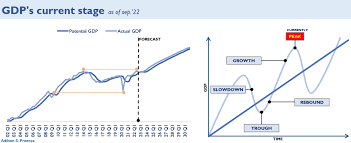
\includegraphics[width=0.5\textwidth]{Imagens/a1i1.png}
        \end{figure}
        \item Enquanto o desenvolvimento econômico estuda as tendências de crescimento do PIB dos países. Comparando tendências de crescimento de países e tentando entender o porque dessa diferença das tendências de crescimento. Não estamos o porque dos ciclos, mas sim entender o porque a tendência "caminha" em uma direção 
\end{itemize}

Para entender melhor, vamos olhar para "\textbf{fatos estilizados}(generalizações simplificadas de fenômenos observados empiricamente.)" de crescimento econômico.

O que determina o "grau de desenvolvimento" de um país ?
\begin{itemize}
    \item Expectativa de Vida
    \item Taxa de homicídio
    \item Anos de escolaridade da população
    \item Renda Per Capita
    \item Desigualdade
    \item Etc.
\end{itemize}

Mas como somos economistas, vamos nos concentrar em:
\begin{itemize}
    \item \textbf{Renda ou PIB Per Capita} : PIB dividido pela população ou Y dividido pela população($\frac{Y}{Pop}$). É uma medida de bem estar.
    \item \textbf{PIB por Trabalhador}: Y divido por L (Força de Trabalho)($\frac{Y}{L}$). Medida de Produtividade.
\end{itemize}

Fazendo $\frac{\frac{Y}{Pop}}{\frac{Y}{L}}$ chegamos na \textbf{taxa de participação}(porcentagem da população que está na força de trabalho), dada pela razão da Força de Trabalha (L) pela População

Podemos assim realizar comparações de rendas internacionais , para isso devemos usar as taxas de câmbio ajustadas pela \textbf{PPP} (\textit{Purchasing Power Parity }, Paridade Poder de Compra(\textbf{PPC})), pois assim conseguimos comparar de maneira justa, sem distorções pelo câmbio e pela cesta de bens.

Para realizar nossas comparações e estudos, utilizaremos a base de dados internacionais da \href{https://www.rug.nl/ggdc/productivity/pwt/}{\textit{Penn World Table}}

\subsection{\textbf{1º Fato Estilizado}}

Há grandes diferenças internacionais de \textbf{nível de renda} per capita. Os países, ou melhor, a renda per capita dos países são muito diferentes entre si ao longo dos anos.

Obviamente, isso se traduz em grandes diferenças internacionais de nível de consumo, como podemos ver na figura abaixo:

\begin{figure}[H]
        \centering
        \caption{Tabela de Comparação de Crescimento} 
        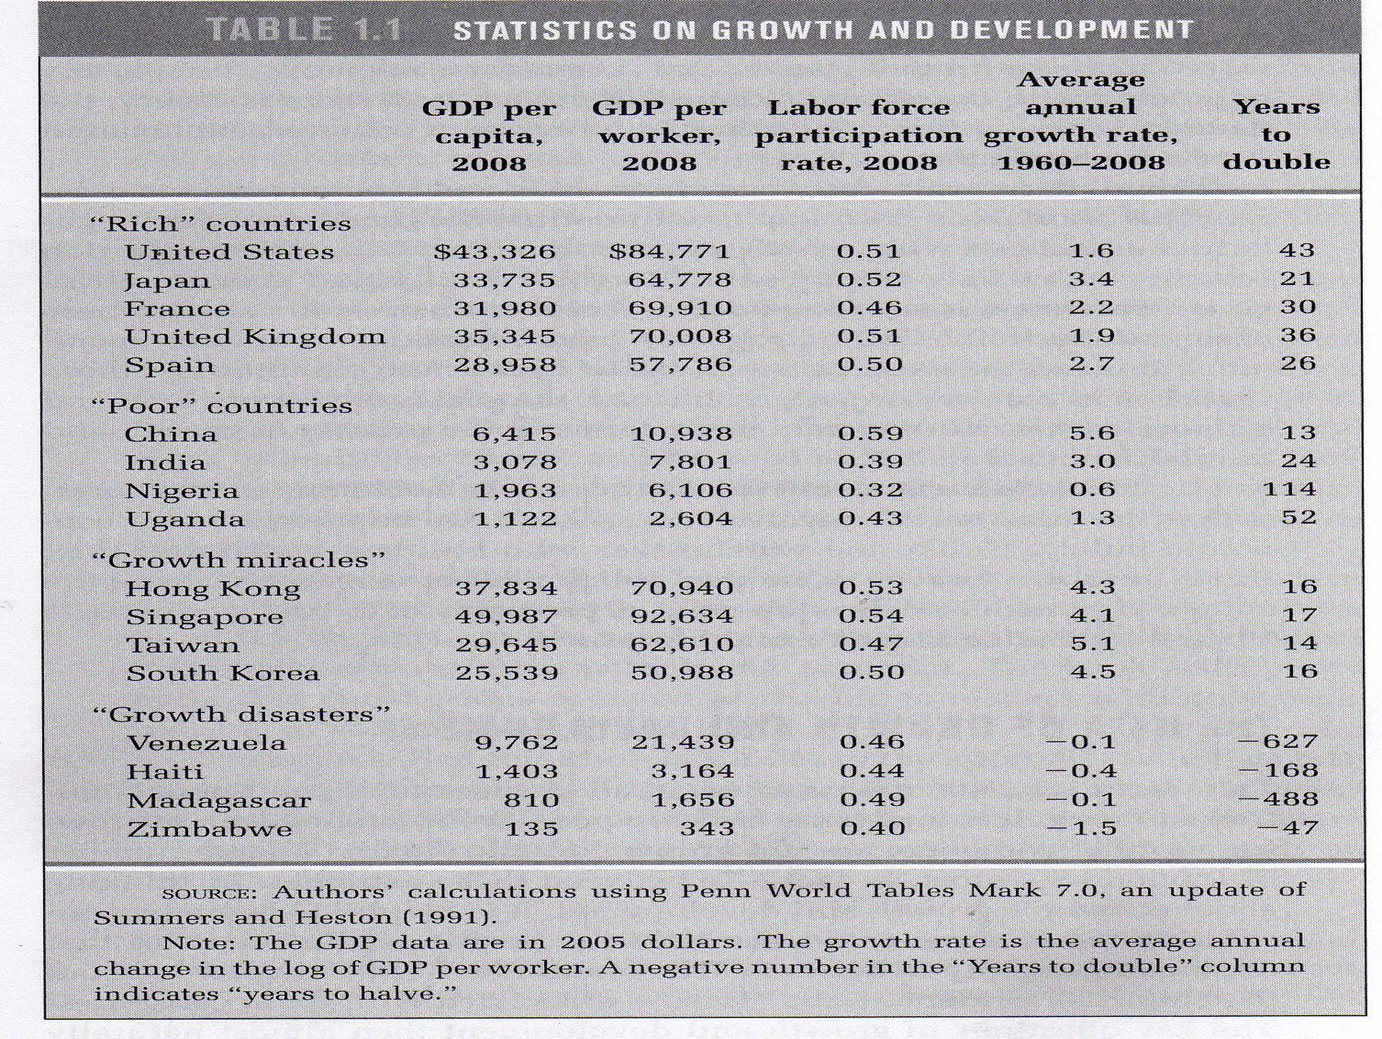
\includegraphics[width=0.5\textwidth]{Imagens/a1i2.png}
\end{figure}

\begin{figure}[H]
        \centering
        \caption{Indicadores World Data Bank} 
        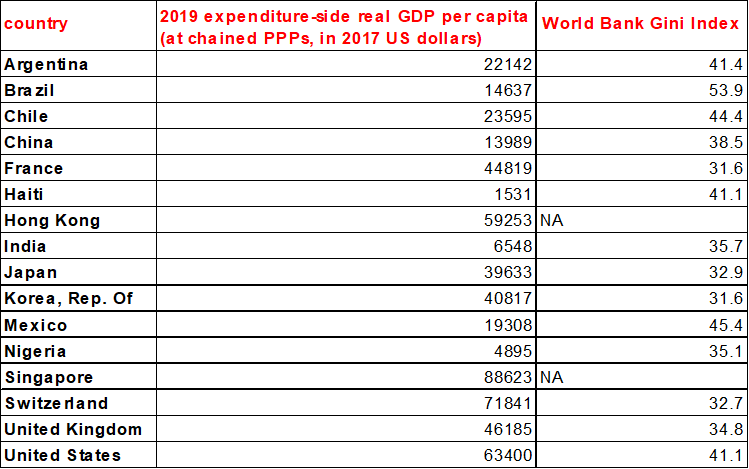
\includegraphics[width=0.5\textwidth]{Imagens/a1i3.png}
\end{figure}

Com essa tabela podemos comparar quais países são mais ricos e mais pobres(em 2019), já que os valores de renda per capita foram ajustadas pela PPP. Por exemplo, comparando a renda dos EUA com a do Haiti, a renda de um estado unidense é quase 41 vezes maior do que a de um haitiano (grandes extremos). Isso é muito atualmente. Comparando os Estados Unidos com o Brasil dá cerca de 4 vezes mais. Mas estamos olhando para o indivíduo médio do país, porém não estamos levando em consideração a grau de desigualdade da população. Por isso que além de colocar as rendas em medidas comparáveis, temos que levar em consideração o \textbf{Índice de Gini}(quanto mais próximo a curva está da linha de 45°, menos desigual é).

O Brasil lidera, nesta tabela, como país mais desigual do mundo, enquanto a França e Coreia do Sul são os mais igualitários.

\begin{figure}[H]
        \centering
        \caption{Curvas de Gini} 
        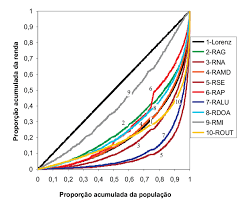
\includegraphics[width=0.5\textwidth]{Imagens/a1i20.png}
\end{figure}

\begin{figure}[H]
        \centering
        \caption{Indicadores World Data Bank} 
        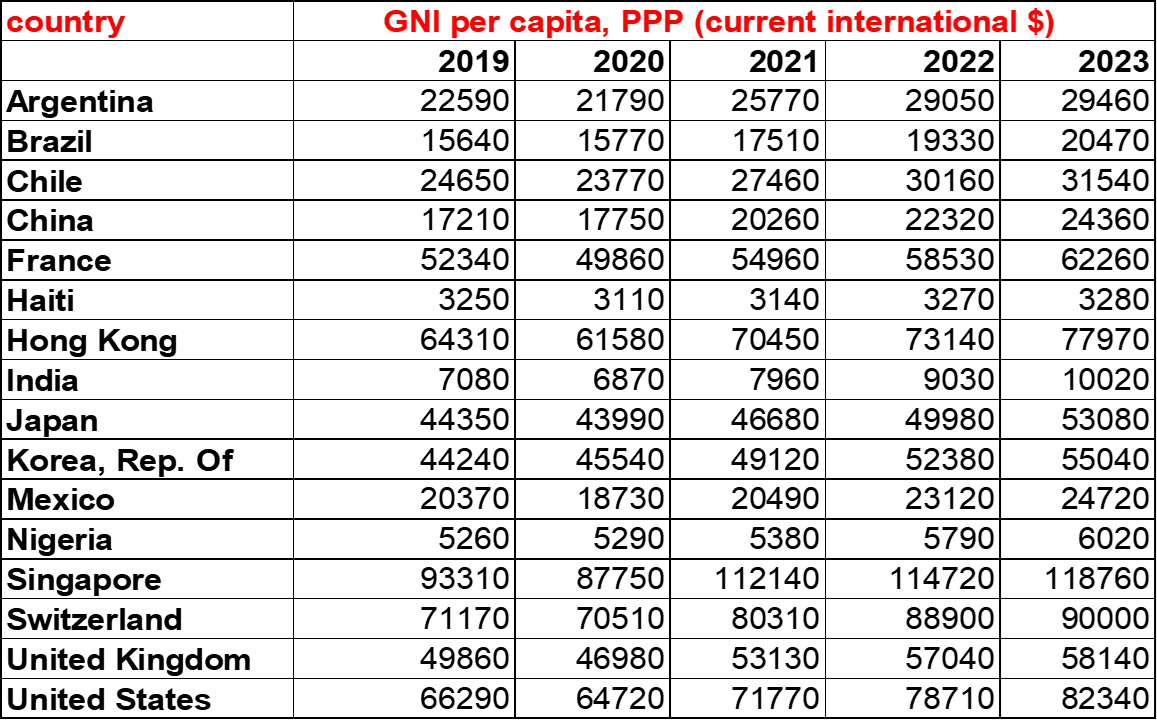
\includegraphics[width=0.5\textwidth]{Imagens/a1i4.png}
\end{figure}

Na tabela acima podemos ver a retração gerada pela pandemia na renda da população média dos países, mas seguida de uma recuperação nos anos anteriores.  

\begin{figure}[H]
        \centering
        \caption{PIB Per Capita e População} 
        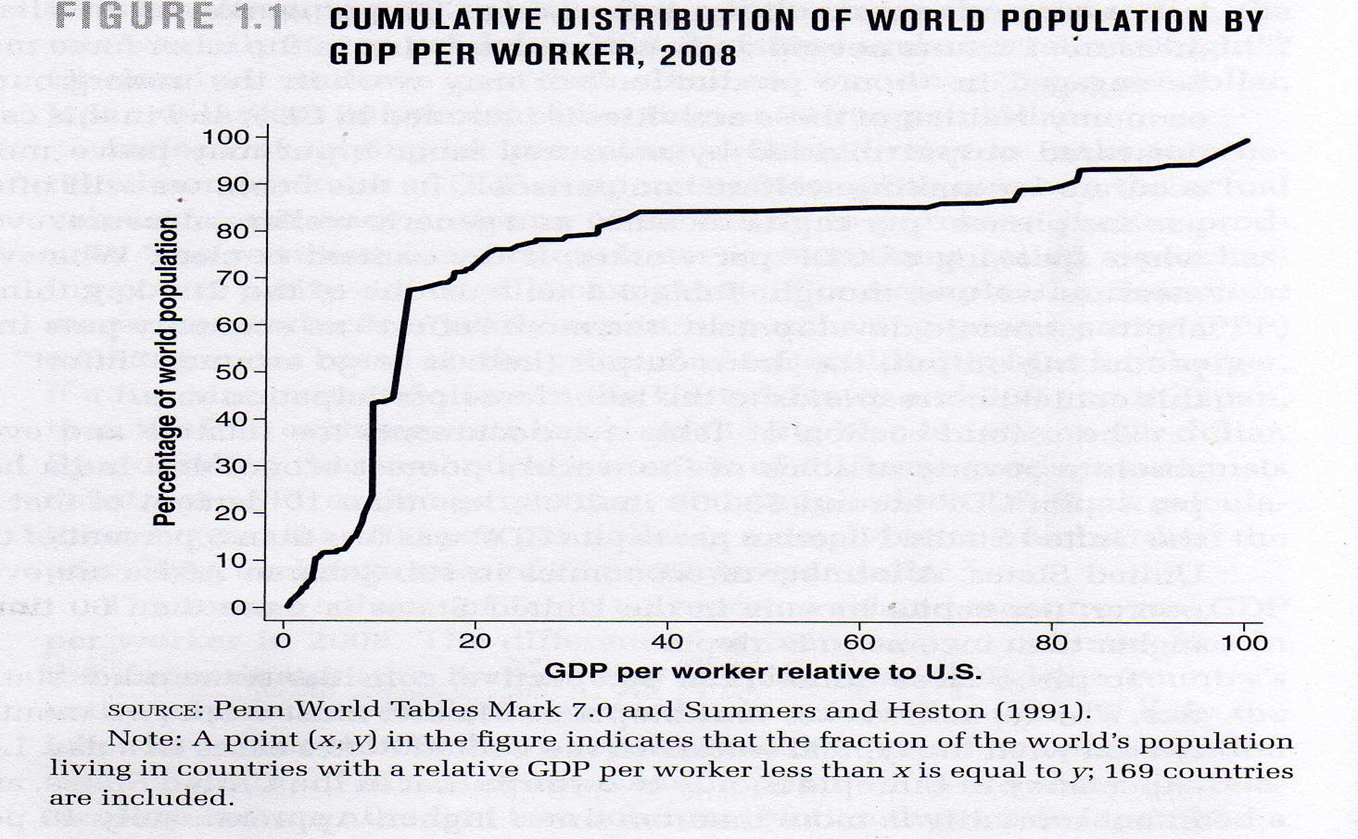
\includegraphics[width=0.5\textwidth]{Imagens/a1i5.png}
\end{figure}

Aqui podemos ver a distribuição da população sobre a renda por trabalhador. Essa FDA(Função de Distribuição Acumulada), só cresce. Pegando no eixo "x" o 20, podemos interpretar como "70\% da população mundo faz o que 20\% do americano faz"

\begin{figure}[H]
        \centering
        \caption{População e PIB por trabalhador} 
        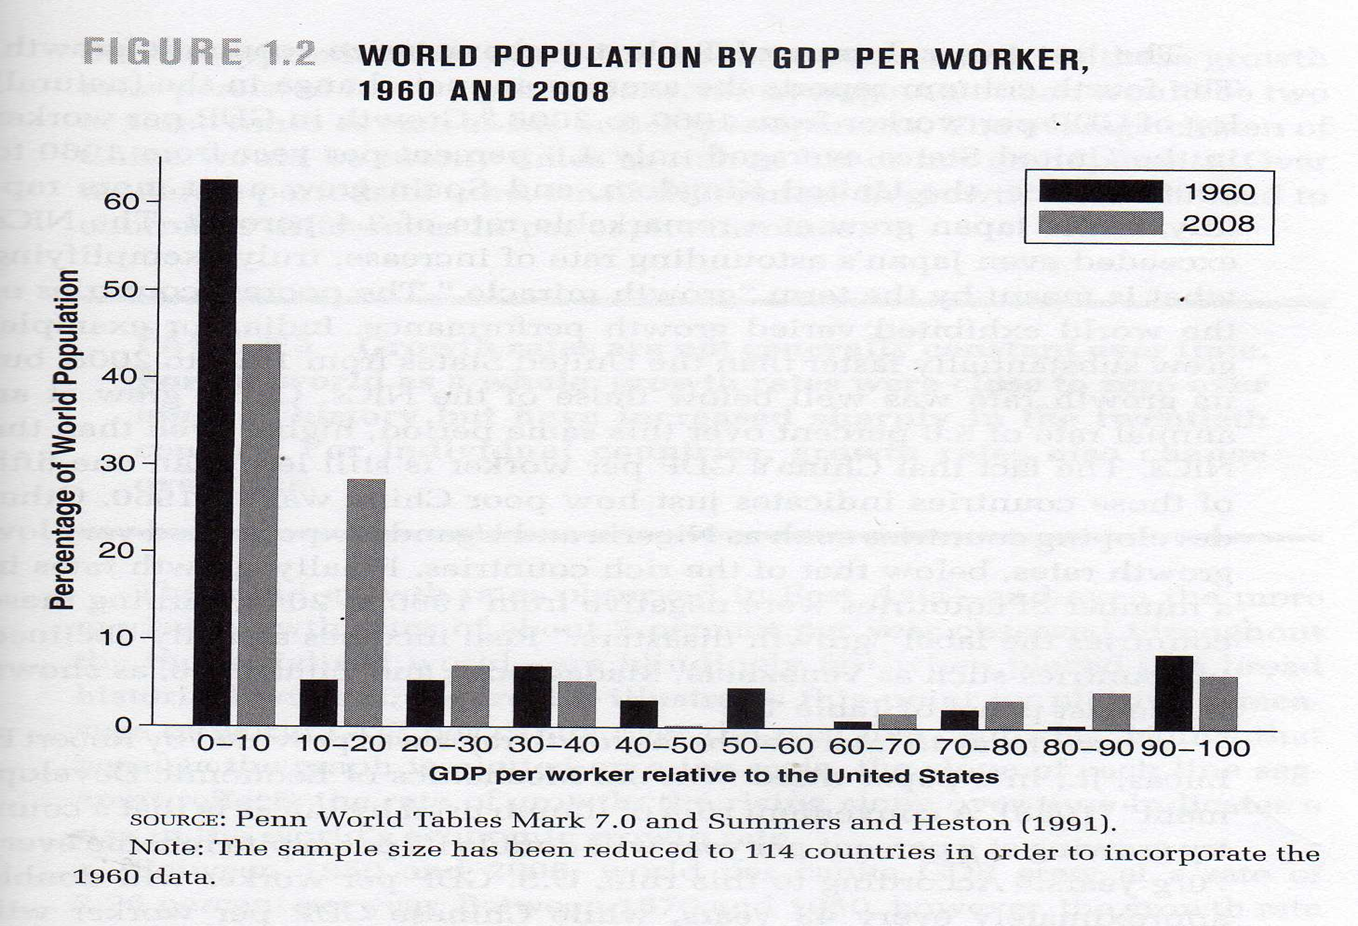
\includegraphics[width=0.5\textwidth]{Imagens/a1i6.png}
\end{figure}

A figura anterior sugere uma melhora na distribuição mundial de renda, de 1960 para cá \begin{itemize}
    \item os países pobres, em média, cresceram mais rápido que os ricos (USA). Será mesmo que houve uma melhora na produtividade global de maneira que os países superaram os ricos?
\end{itemize} 

\subsection{\textbf{2º Fato Estilizado}}
Há grandes diferenças internacionais de taxas de crescimento de longo prazo \begin{itemize}
    \item países com diferentes “\textit{performances}”
    \item calculo feito da seguinte forma : $g_y \approx \frac{ln(y_{i,2010})-ln(y_{i,1960})}{50}$
\end{itemize}
\begin{figure}[H]
        \centering
        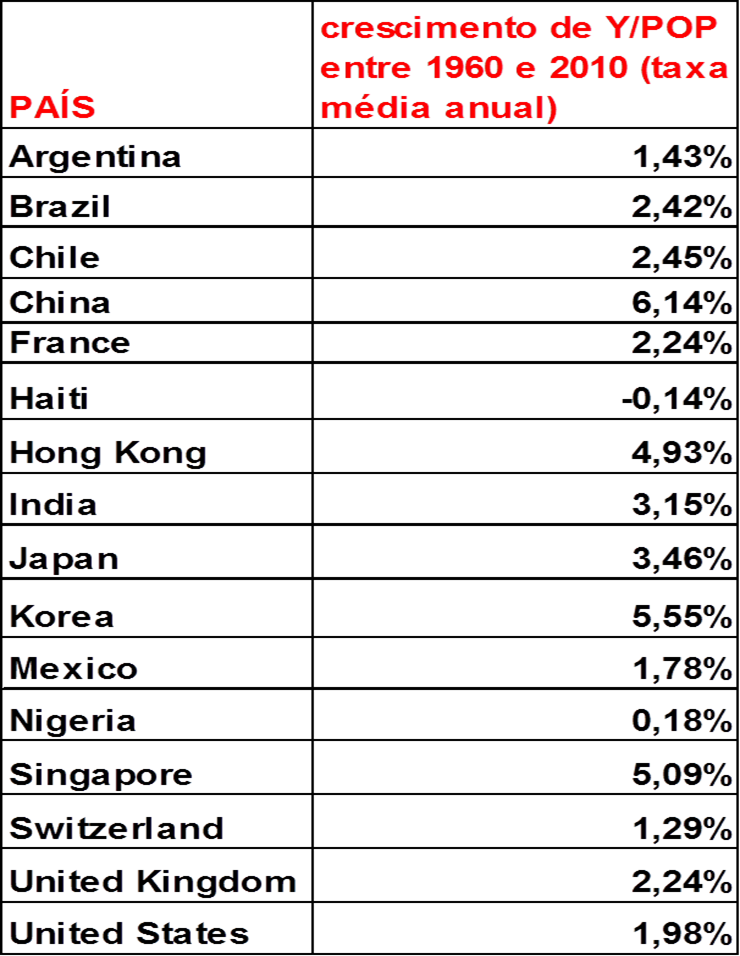
\includegraphics[width=0.5\textwidth]{Imagens/a1i7.png}
\end{figure}

China possui a taxa de crescimento mais alta dos últimos 50 anos, seguido da Coreia do Sul. Interpretando a taxa da Coreia do Sul ($(1,055)^{50}=14,54$ de crescimento). O Haiti regrediu nos últimos 50 anos.

Uma grande preocupação é: será que os países mais pobres tendem a “alcançar” os mais ricos ?

Colocando de outra maneira, considerando um típico “país rico” e um típico “país pobre”, será que a razão $\frac{(Y/POP)_{pobre}}{(Y/POP)_{rico}}$ tende a aumentar com o tempo ? \begin{itemize}
    \item caso sim, dizemos haver \textbf{convergência} internacional de renda per capita !
\end{itemize}

Voltemos ao nosso exemplo com 16 países:
\begin{figure}[H]
        \centering
        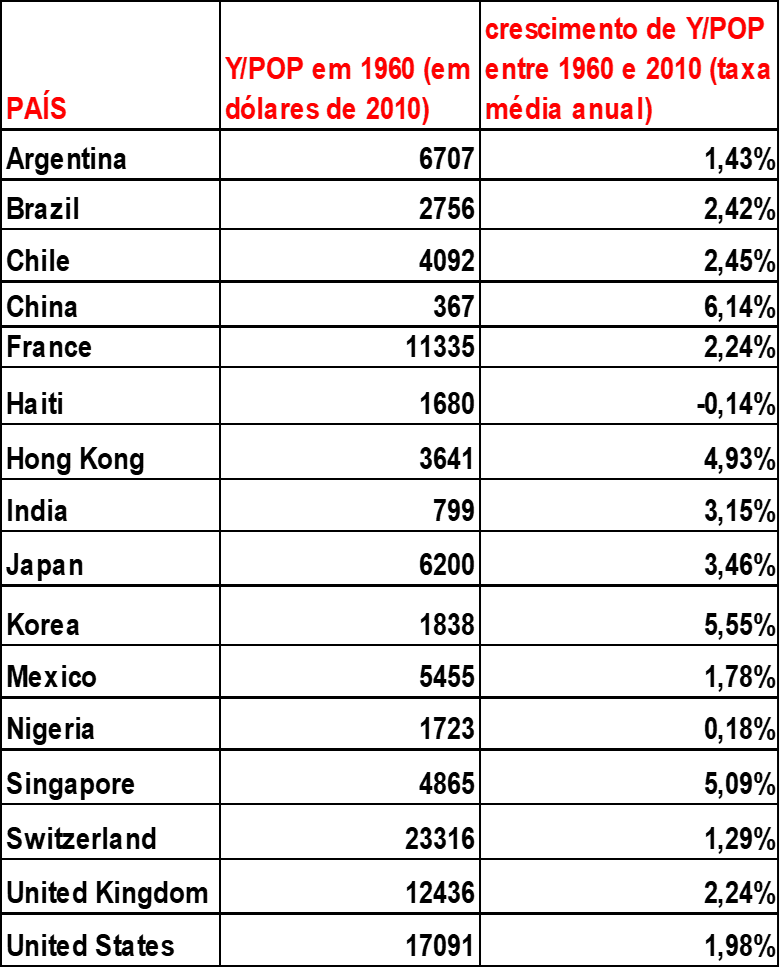
\includegraphics[width=0.5\textwidth]{Imagens/a1i8.png}
\end{figure}

Inspecionando a tabela acima, vemos que em 1960 o Brasil, a China e a Índia eram mais pobres que os USA, e de fato esses países cresceram mais que os USA de 1960 a 2010 $\rightarrow$ \textbf{convergência}!!

Mas o México, o Haiti e a Nigéria eram mais pobres que os USA em 1960, e cresceram menos que os USA de 1960 a 2010  $\rightarrow$ \textbf{divergência}!!

A Suiça era mais rica que os Estados Unidos em 1960, logo era convergiu. Ou podemos interpretar a Suiça como o país rico e os Estados Unidos como mais probre, e repitir a conta, chegando no mesmo resultado. 

Olhando para (quase) todos os países do mundo, o que prevalece: convergência ou divergência ? 

Para dar uma resposta, vamos regredir a taxa média de crescimento anual da renda per capita (entre 1960 e 2010) contra a renda per capita inicial (de 1960), numa amostra de 111 países da Penn World Table:

\textbf{Regressão}:
$g_{yi}= \beta_0+\beta_1y_{i,1960}+\varepsilon_i$

\textbf{Estimativas}:\begin{itemize}
    \item $\hat{\beta_0}$=0,0185 com p-valor $\approx$ 0
    \item $\hat{\beta_1}$=0,0000002332 com p-valor $\approx$ 0,46
    \item Ou seja, há uma evidência pouco significativa de \textbf{divergência} (afinal, beta 1 estimado $>$ 0 …) !!
\end{itemize}

\begin{figure}[H]
        \centering
        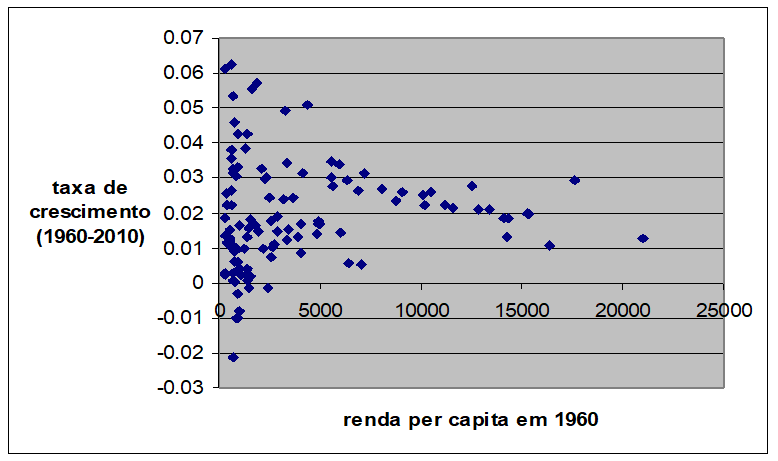
\includegraphics[width=0.5\textwidth]{Imagens/a1i9.png}
\end{figure}

No entanto, certos grupos de países apresentam convergência  $\rightarrow$ “clubes” de convergência

\begin{figure}[H]
        \centering
        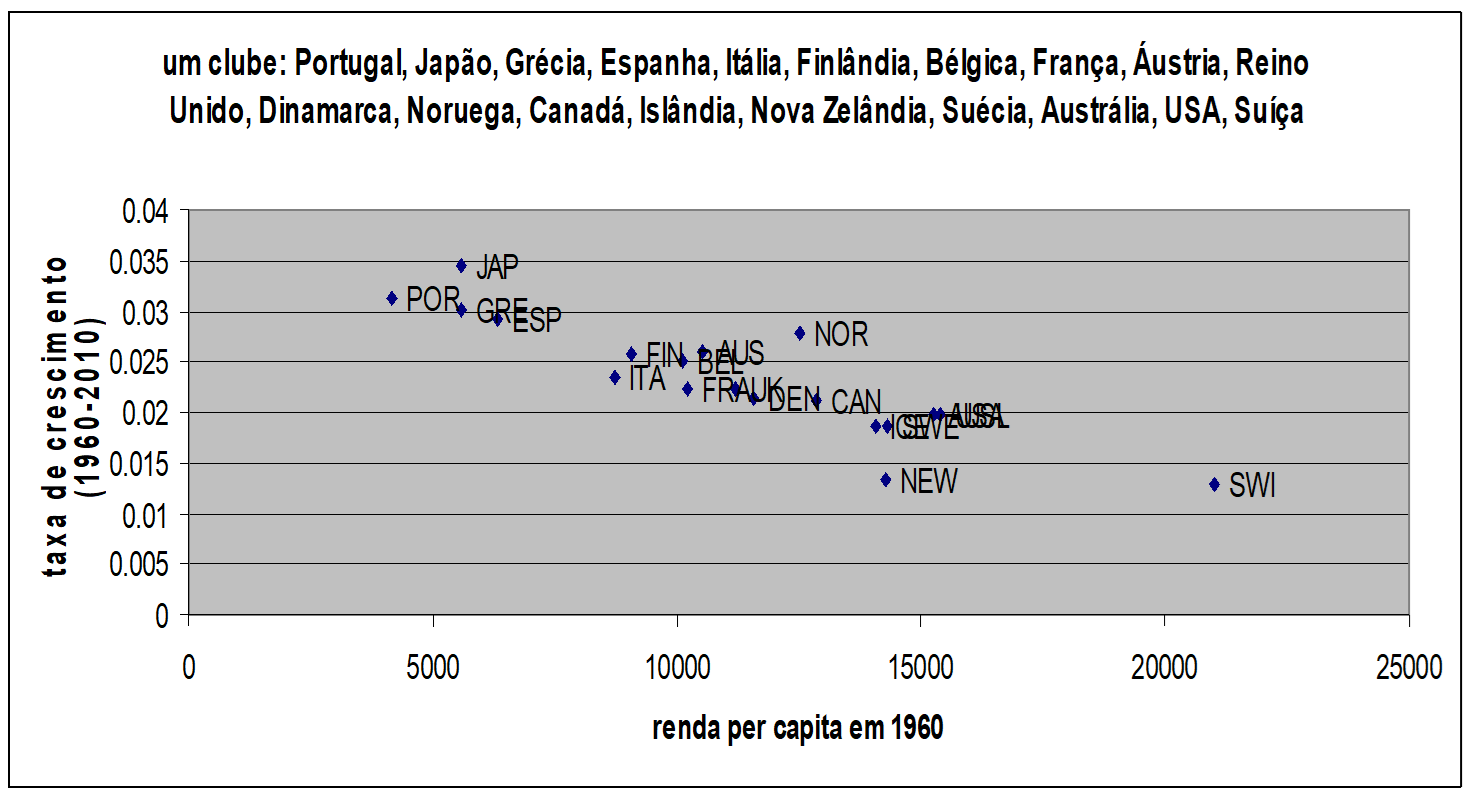
\includegraphics[width=0.5\textwidth]{Imagens/a1i10.png}
\end{figure}

Por que um gráfico mostra que há divergência e outro mostra convergência? Simples, estamos levando em consideração a população, que trazem "pesos" distintos para as comparações. Lembre, China e Índia juntas possuem praticamente metade da população mundial, e eles foram as duas nações que mais cresceram no período analisados. 

\subsection{\textbf{3º Fato Estilizado}}
Em geral, as taxas de crescimento não são constantes ao longo do tempo.

Para o mundo como um todo, e de um ponto de vista de muito longo prazo, a taxa de crescimento era quase zero até a Revolução Industrial, e aumentou consideravelmente no séc. XX:

\begin{figure}[H]
        \centering
        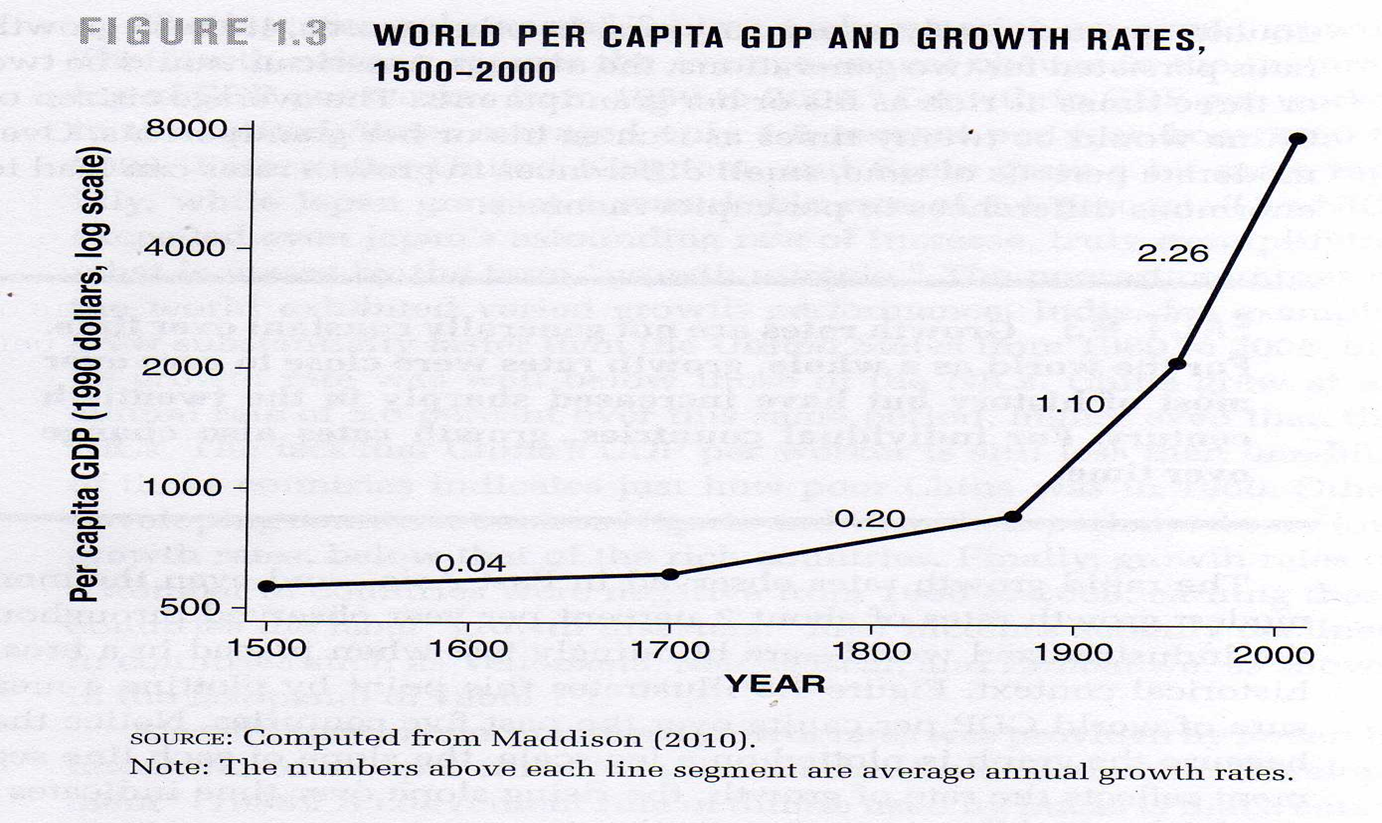
\includegraphics[width=0.5\textwidth]{Imagens/a1i11.png}
\end{figure}
Taxas de crescimentos anuais são calculadas da seguinte forma no gráfico acima:
$$\frac{d}{dt}ln(y_t)=\frac{1}{y_t}\frac{d}{dt}y_t=g_{y_t}$$

Para um mesmo país, a taxa de crescimento varia de período a período:

\begin{figure}[H]
        \centering
        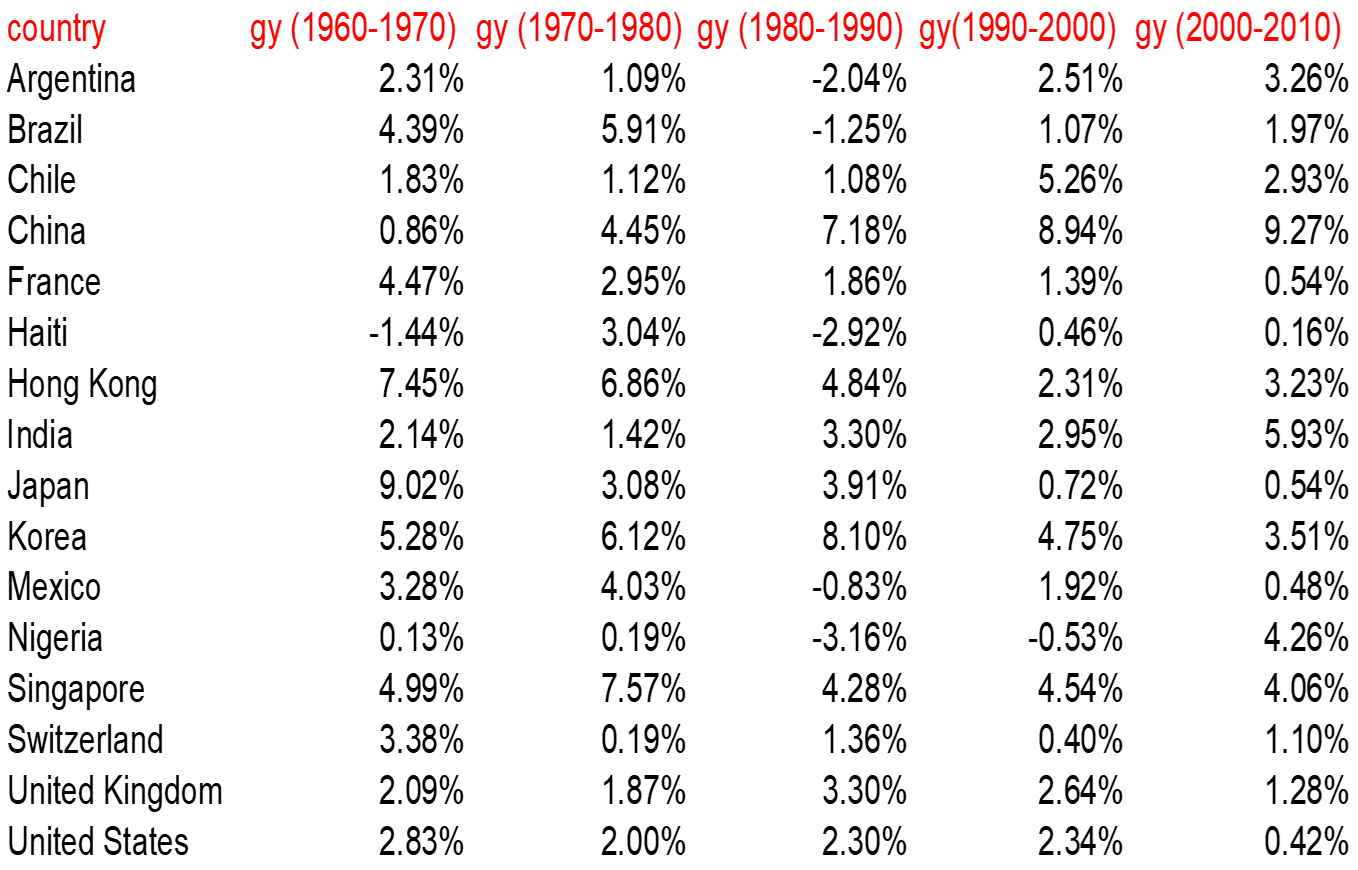
\includegraphics[width=0.5\textwidth]{Imagens/a1i12.png}
\end{figure}

O que aconteceu em 1980 que quebrou países como Brasil e México? Paul Volcker, presidente do \textbf{FED} aumentou drasticamente a taxa de juros para combater um aumento da inflação, e esses países pegaram dinheiro emprestado dos EUA, com o aumento da taxa de juros as dívidas desses países disparam, o que gerou grandes recessões dessas economias. 

Juntando os fatos '2' e '3', temos o seguinte “\textbf{corolário}(conclusão lógica)”:

\subsection{\textbf{4º Fato Estilizado}}
A posição relativa de um país na distribuição mundial de renda não é imutável \begin{itemize}
    \item ele pode passar de pobre a rico (South Korea de 1950 p/ cá)
    \item ele pode passar de rico a médio (Argentina no séc. XX)
\end{itemize}

A situação atual de cada país está sujeita a volatilidade do tempo, posições podem ser trocadas, destrocadas ou mantidas. Não é certeza que o jeito que você começa que você vai terminar.

\subsection{\textbf{5º Fato Estilizado}}
Kaldor(inseriu a econometria para tentar enxergar relações por via dos dados), para uma economia em \textit{steady-state(economia capitalista madura)}, como os USA no séc. XX:\begin{enumerate}
    \item taxa real de retorno do capital ($r$) constante ao longo do tempo(traz uma certeza para investidores, bancos, empresas, etc para realizar investimentos de longo)
    \item participações do capital ($\frac{rK}{Y}$) e do trabalho ($\frac{w.L}{Y}$) na renda nacional constantes ao longo do tempo
    \item As duas anteriores implicam $\frac{K}{Y}$relação capital-produto cte.
    \item taxa de crescimento da renda per capita constante ao longo do tempo ($\approx$2\% a.a.)  \item Kaldor acabou por descobrir que $\frac{rK}{Y} \approx\frac{1}{3}$ e $\frac{wL}{Y} \approx\frac{2}{3}$
\end{enumerate}

\subsection{\textbf{6º Fato Estilizado}}
Correlação positiva entre taxa de crescimento do PIB (Y) e taxa de crescimento do volume de comércio internacional (EX + IM).

\begin{figure}[H]
        \centering
        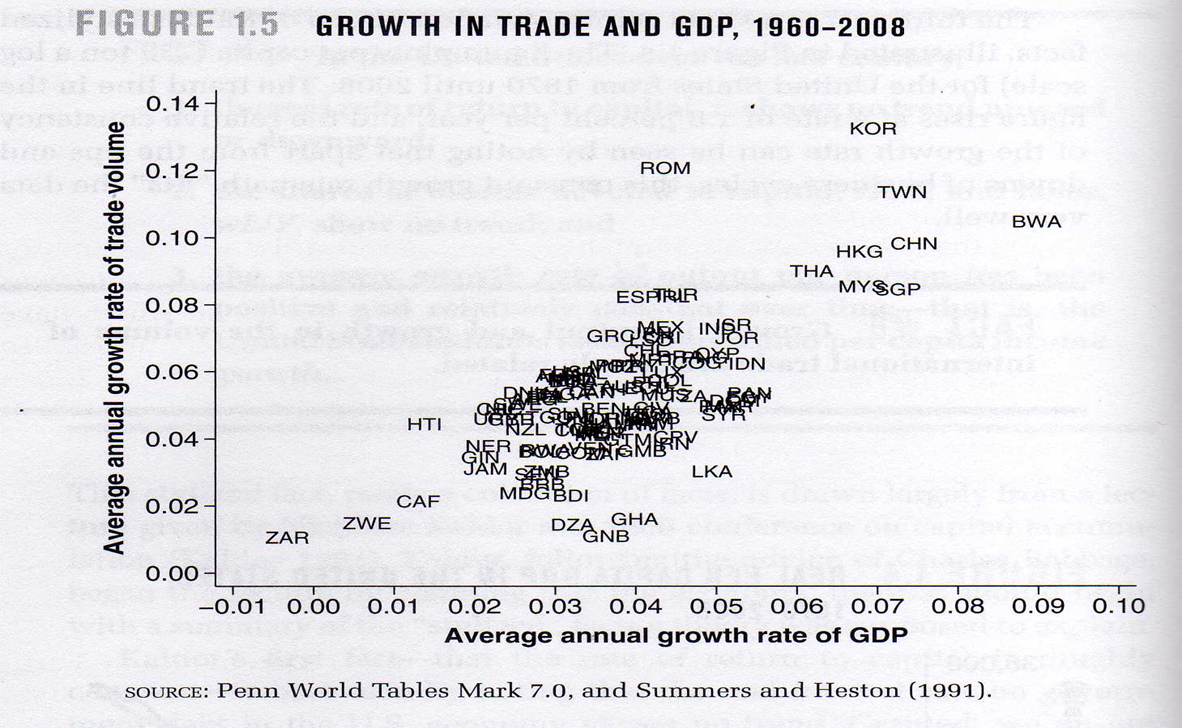
\includegraphics[width=0.5\textwidth]{Imagens/a1i13.png}
\end{figure}

Mas cuidado !(não estamos sugerindo causalidade, nem que economias ricas são mais abertas)

\begin{figure}[H]
    \centering
    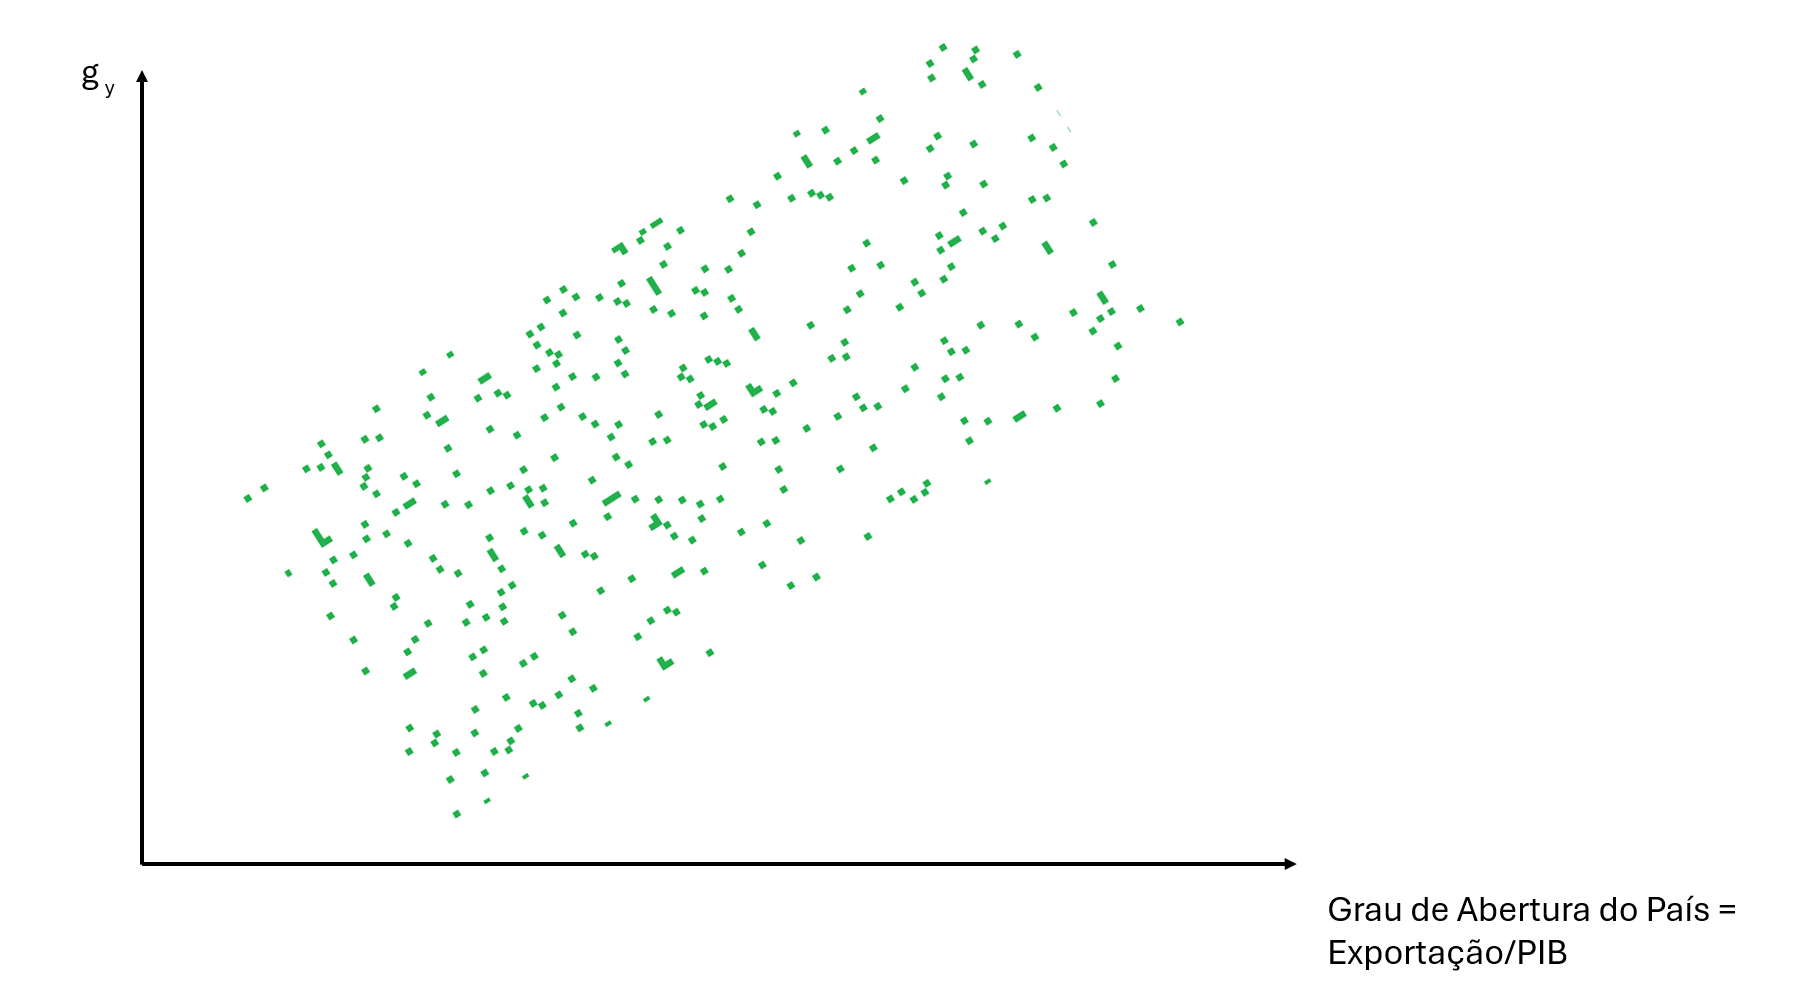
\includegraphics[width=0.5\linewidth]{Imagens/a1i21.png}
\end{figure}

A. Alesina em \textit{HandBook of Economic Growth} estabeleceu uma relação crescimento de um país contra o seu grau de abertura($\frac{Ex}{Y}$). 

\subsection{\textbf{7º Fato Estilizado}}
Tanto o capital, como trabalhadores qualificados e não-qualificados tendem a migrar de países/regiões “pobres”, atrasados, para países/regiões “ricos, desenvolvidos.\begin{itemize}
    \item trabalho não-qualificado … OK
    \item capital e trabalho qualificado  … puzzle ! Teoricamente o capital teria que sair do país desenvolvido ir para o subdesenvolvido e não o contrário, mas porque o inverso é o que acontece? Simples, países já desenvolvidos são mais seguros. (Lucas)
\end{itemize}

Temos que lembrar também que temos espaços geográficos e acesso a recursos naturais. Mas vamos focar em capital e trabalho.

E ainda mais que podemos dividir a força de trabalho pode ser dividida\[L=\underbrace{L_s}_{\text{Especializado}}+\underbrace{L_u}_{\text{Não Especializado}}
 \]
 
\textit{Afinal, diferenças internacionais de remunerações dos fatores deveriam refletir diferenças de escassez relativa. $\rightarrow$ como explicar ? Instituições, retornos crescentes de escala ?}

\subsection{\textbf{Como explicar esses fatos ?}}\begin{enumerate}
    \item modelo de Solow (1956)
    \item modelo de Solow com capital humano – Mankiw, Romer e Weil (1992)
    \item modelos de crescimento endógeno – Romer (1990), Grossman \& Helpman (1991), Aghion \& Howitt (1992)
\end{enumerate}

Cada modelo enfatiza um aspecto/fator diferente … logo, esses modelos podem ser vistos como complementares, embora (como sempre) os economistas acadêmicos discordem quanto à relevância teórica e empírica de cada um.

Modelo de Solow e variações $\rightarrow$ ênfase na \textbf{acumulação} de \textbf{capital físico} (máquinas, infra-estrutura, etc.) e na acumulação de \textbf{capital humano} (instrução, qualificação dos trabalhadores)

Modelos de crescimento endógeno  $\rightarrow$ ênfase nos determinantes do \textbf{progresso tecnológico}

Dada sua ênfase, cada modelo também leva a diferentes recomendações (ou “corolários”) em \textbf{termos de políticas econômicas para promover o crescimento}\begin{itemize}
    \item modelo de Solow e variações  $\rightarrow$ estimular a \textbf{poupança e o investimento (FBCF(formação Bruta de Capital Fixo)) ; educação}
    \item modelos de crescimento endógeno  $\rightarrow$ incentivos para \textbf{pesquisa científica}; subsídios para \textbf{P\&D} pelas empresas; leis de \textbf{patentes}
\end{itemize}

O modelo explica bem os dados  $\rightarrow \frac{I}{Y}=\frac{S}{Y}=s ; Como \ diria \ Solow$:
Não há uma relação bem obvia vendo esses dados, mas existe, veremos mais afrente.

\begin{figure}[H]
        \centering
        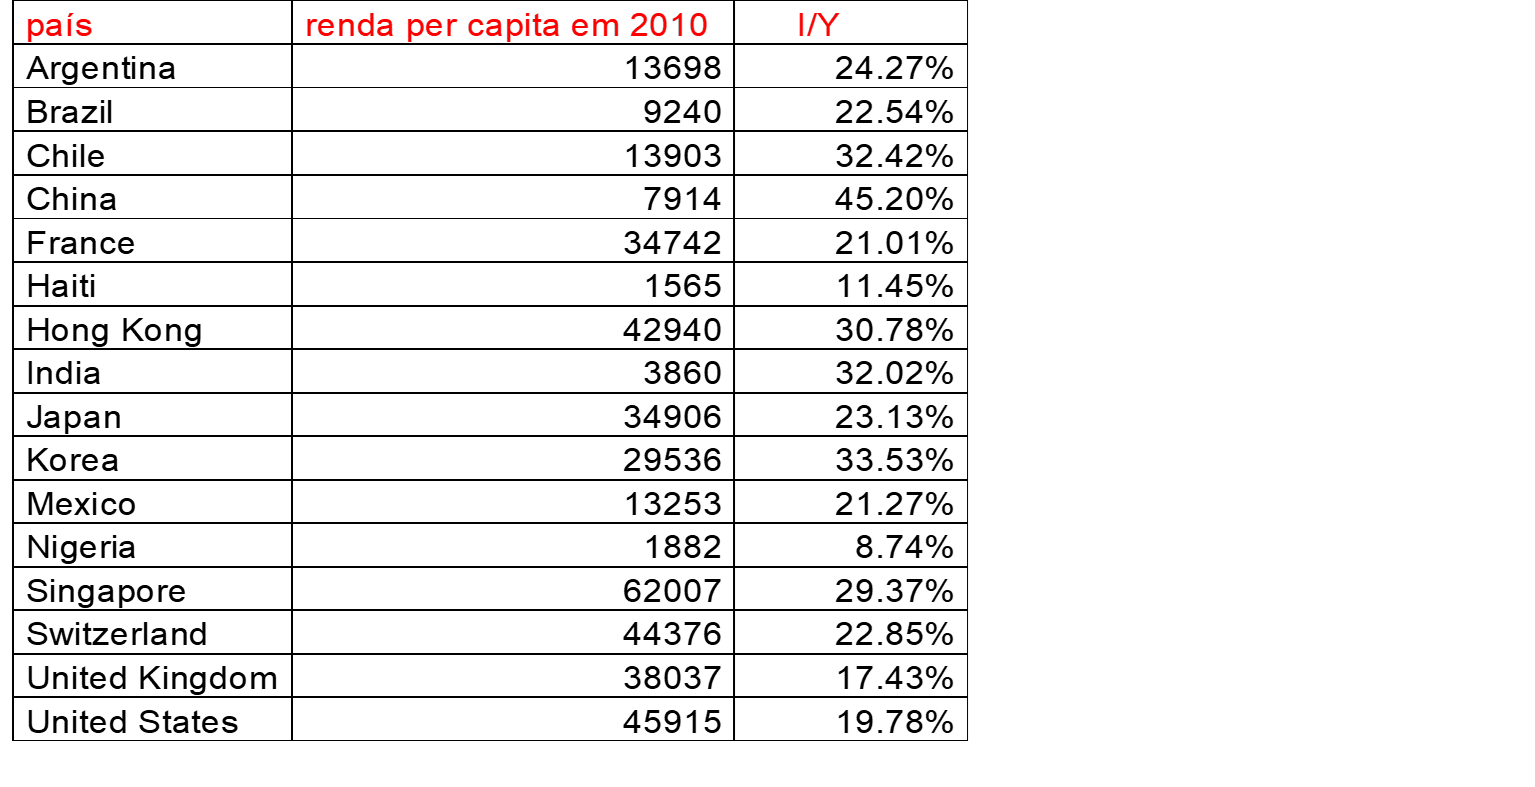
\includegraphics[width=0.5\textwidth]{Imagens/a1i14.png}
\end{figure}

A taxa de poupança ou investimento $\frac{I}{Y}$ não parece explicar muito bem o nível de renda per capita.

Economias ricas “maduras”, como os EUA , a Suíça e o Reino Unido, apresentam $\frac{I}{Y}$ em torno de 20\%.

Países em rápido crescimento, como a China, a Coreia e Hong Kong, apresentam $\frac{I}{Y}$ mais alta.

Olhando para 111 países (Penn Table):

\begin{figure}[H]
        \centering
        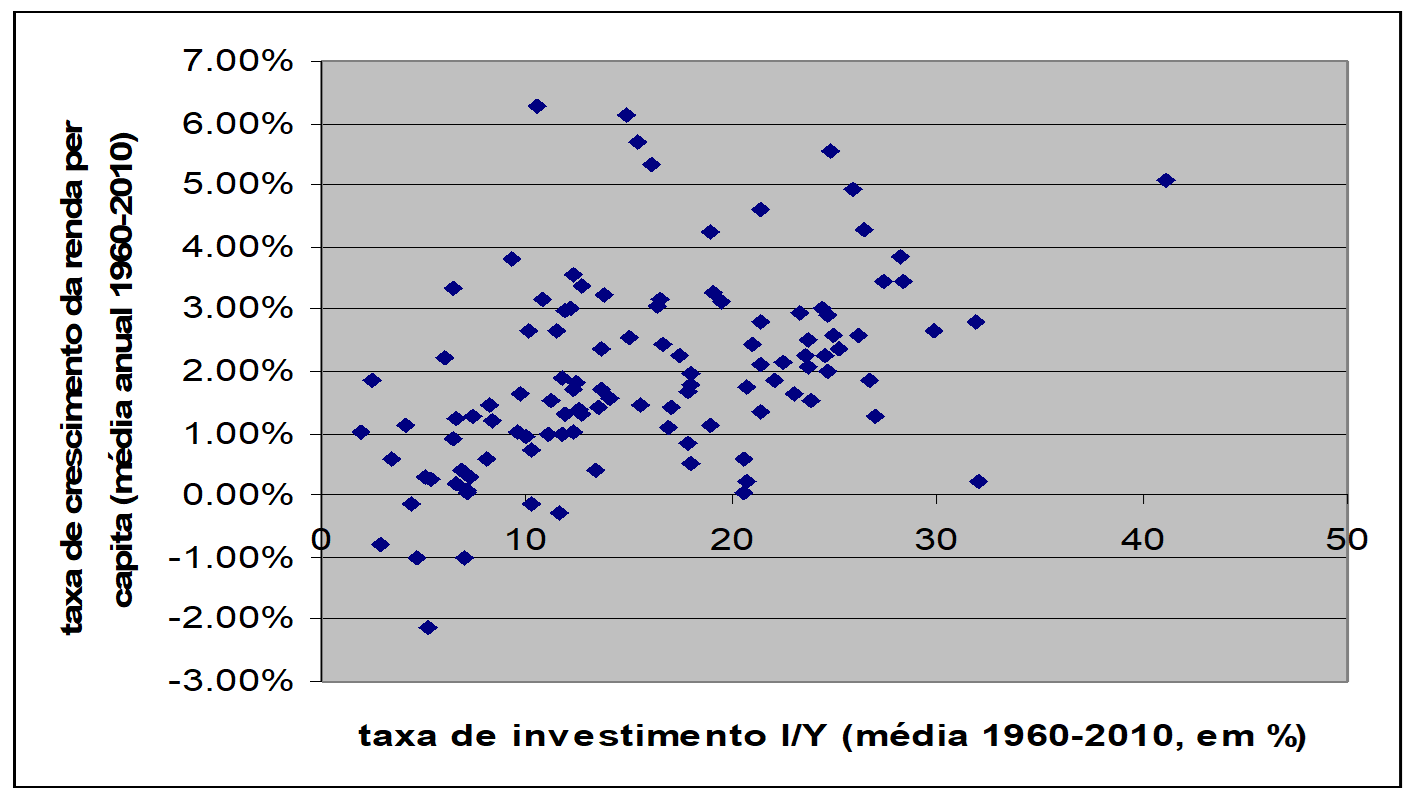
\includegraphics[width=0.5\textwidth]{Imagens/a1i15.png}
\end{figure}

O modelo explica bem os dados ? $\rightarrow$ Educação(fonte: PWT e Barro \& Lee database)
\begin{figure}[H]
        \centering
        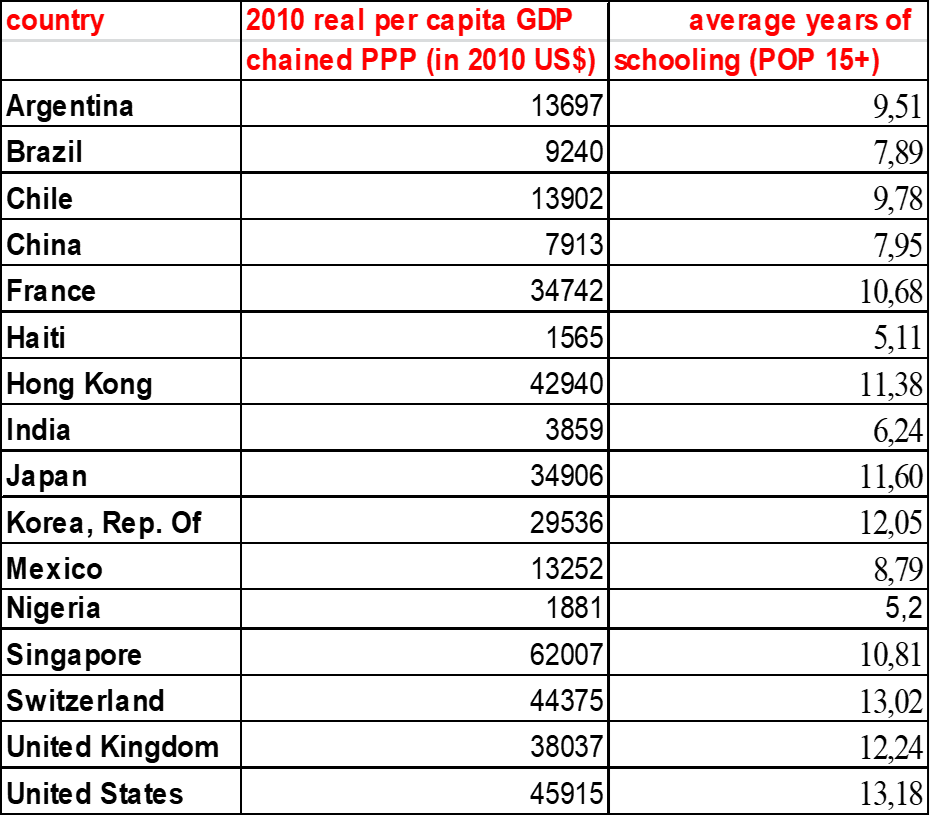
\includegraphics[width=0.5\textwidth]{Imagens/a1i16.png}
\end{figure}




Anos de estudo: média da POP com 15 anos de idade ou + (Fonte: Barro \& Lee)

\begin{figure}[H]
        \centering
        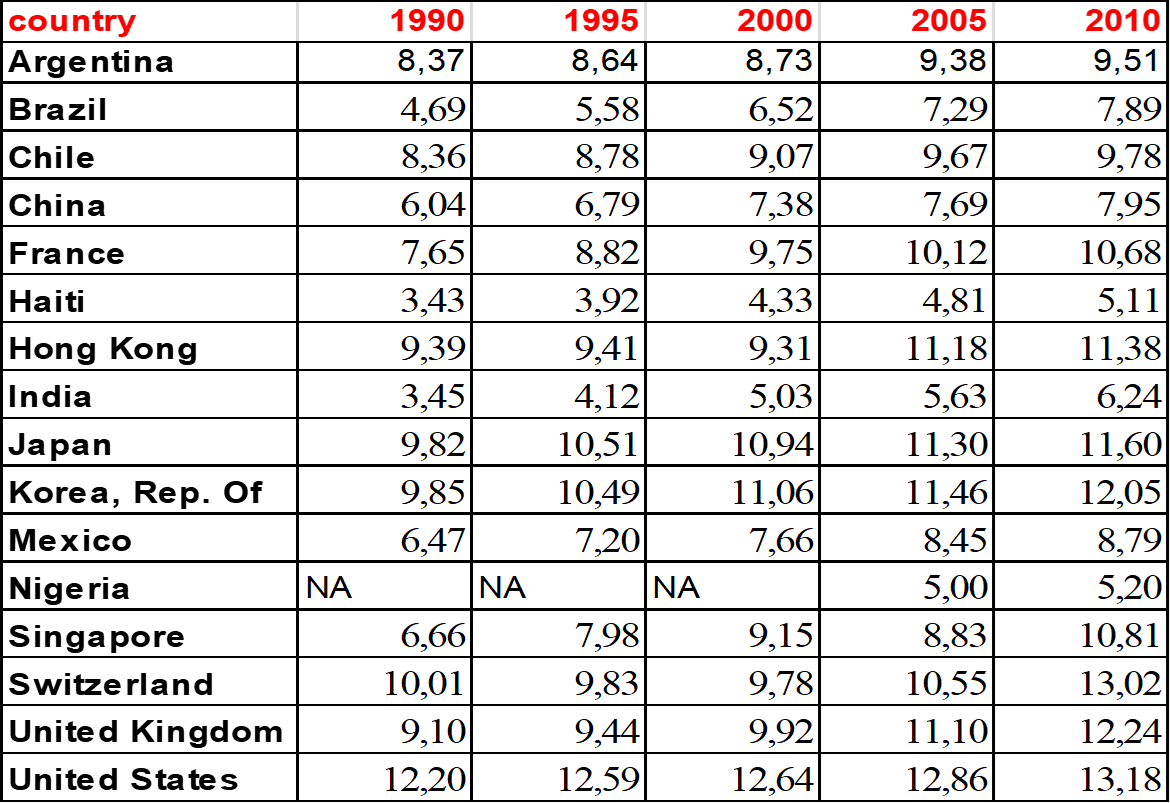
\includegraphics[width=0.5\textwidth]{Imagens/a1i17.png}
\end{figure}

Olhando para 130 Países (Penn Table e Barro \& Lee):

\begin{figure}[H]
        \centering
        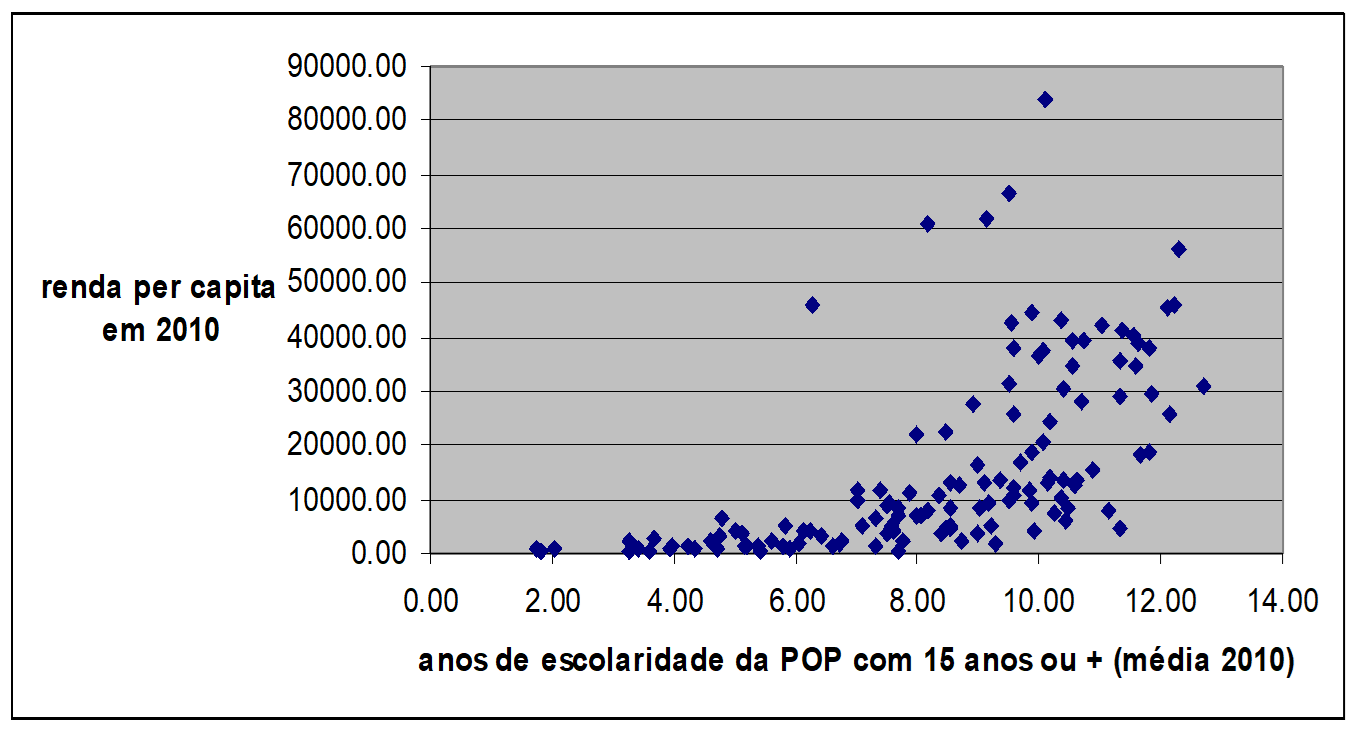
\includegraphics[width=0.5\textwidth]{Imagens/a1i18.png}
\end{figure}

O modelo explica bem os dados ?  $\rightarrow$ \textbf{tecnologia}


\begin{figure}[H]
        \centering
        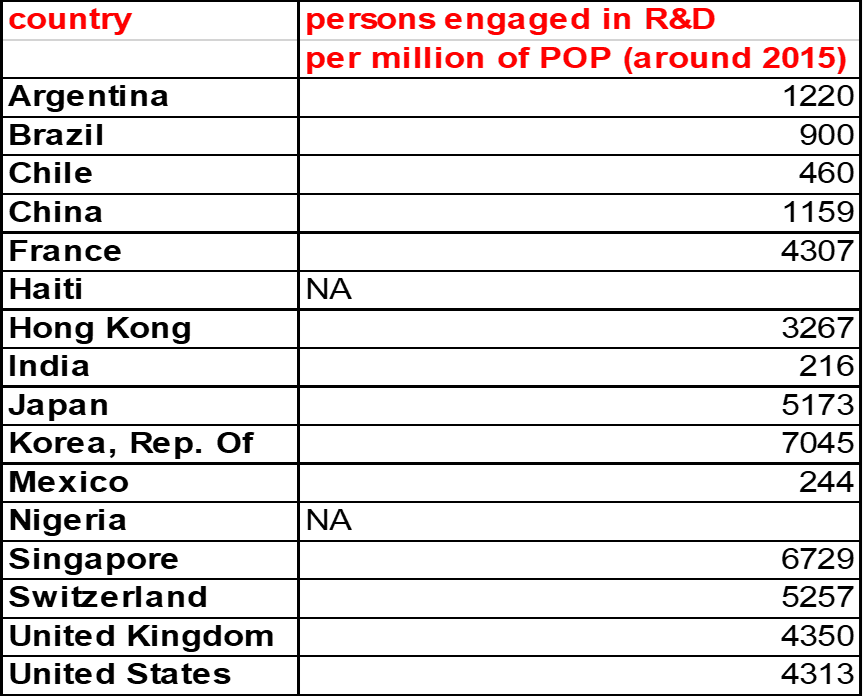
\includegraphics[width=0.5\textwidth]{Imagens/a1i19.png}
\end{figure}

\newpage
\section{\textbf{O Modelo de Solow- Sem Progresso Tecnológico e Sem Capital Humano}}
O modelo de Solow possuí três versões:\begin{enumerate}
    \item \textbf{sem} progresso tecnológico e \textbf{sem} capital humano \textbf{Capítulo 2} \(\rightarrow\) Ênfase na acumulação de capital físico
    \item \textbf{com} progresso tecnológico e \textbf{sem} capital humano \textbf{Capítulo 2}
    \item \textbf{com} progresso tecnológico e \textbf{com} capital humano \textbf{Capítulo 3}
\end{enumerate}
\subsection{Função de Produção}
\(Y=F(K:\text{capital físico},L:\text{trabalho})\) é uma função de produção\begin{itemize}
    \item \textbf{Derivadas}\begin{enumerate}
        \item \(\frac{\partial F}{\partial K}>0\), \(\frac{\partial F}{\partial L}>0\), \(\frac{\partial^2 F}{\partial^2 K}<0\) e \(\frac{\partial^2 F}{\partial^2 L}<0\), os fatores que determinam o produto agregam positivamente para seu aumento(1º derivada), mas os aumentos vem sempre a taxas menores(2º derivada).
        \item \(\frac{\partial (\frac{\partial F}{\partial K})}{\partial L}\) e \(\frac{\partial (\frac{\partial F}{\partial KL})}{\partial K}>0\), o produto marginal dos fatores do produto(1º derivada) tem impactos maiores a medida que o outro fator aumenta(2º derivada).
    \end{enumerate}
    \item \textbf{Homogeneidade}\begin{enumerate}
        \item F(\(\cdot\)) é \(H(1)\)(homogenia de grau 1), logo pelo teorema de Euler, temos que \[K\underbrace{\frac{\partial F}{\partial K}}_\text{taxa real de juros}+L\underbrace{\frac{\partial F}{\partial L}}_\text{salários dos trabalhadores}= F(K,L)\]
    \end{enumerate}
\end{itemize}
\subsubsection{\textbf{Exemplo}}
\textbf{Kaldor} dizia que \(\approx1/3\) vai para os donos de capital. Logo o \(\alpha \approx 1/3\).

\[
Y=F(K,L)= \underbrace{K^{\alpha}L^{1-\alpha}\ ; \ 0<\alpha<1}_{Cobb-Douglas} \Rightarrow \underbrace{\frac{Y}{L}}_{Produto por Trabalhador}\equiv y={(\frac{K}{L})}^{\alpha}\Rightarrow \mathcal{k}^\alpha \equiv f(\mathcal{k}) \ \ \ \ \textbf{(1)}
\]

\[
\underbrace{\frac{\partial Y}{\partial K}}_\text{r ou \(PMg_k\)}=\alpha K^\alpha L^{1-\alpha}K^{-1}=\alpha YK^{-1}
\]

\[
\text{Agora, a participação do K na renda}\frac{PMg_kK}{Y}=\alpha \approx\frac{1}{3} 
\]

Ao longo do tempo, o movimento do estoque de capital por trabalhador, \(R\), depende do movimento de \(K\) e \(L\): \(\dot{\mathcal{k}_t}\equiv\frac{dR_t}{dt}\)

Bem:
\[
\dot{\mathcal{k}} = \dot{\left(\frac{K}{L}\right)} = \frac{\dot{K}L - K\dot{L}}{L^2} = \frac{\dot{K}}{L} - \mathcal{k}\frac{\dot{L}}{L} \equiv \frac{\dot{K}}{L} - \mathcal{k} \underbrace{n}_{\text{tx. de cres. populacional} \equiv \frac{\dot{N}}{N}}\ \ \ \ \textbf{(2)}
\]

Observação; assumiremos a hipótese de que \(L=bN\), onde \(b\) é a taxa de participação da mão de obra ou força de trabalho, além disso \(0<b<1 \ ; \ \frac{db}{dt}=0 \). Outra hipótese fundamental de Solow é que poupança é igual a investimento são dados exógenos:
\[
\dot{K}\equiv\frac{dk}{dt}=\underbrace{\underbrace{\mathcal{s}}_{\text{tx de poupança}}Y}_{Investimento}-\underbrace{{\underbrace{\delta}_{\text{tx de depreciação do capital}}K}}_{Depreciacao} \ \ \ \ \textbf{(3)}
\]

Substituindo a \textbf{(3)} e \textbf{(2)}
\[
\dot{\mathcal{k}}=\underbrace{\mathcal{s}y}_{construcao}-\underbrace{\mathcal{k}(\delta+n)}_{destruicao} \ \ ou \ \ \dot{\mathcal{k}}=\underbrace{\mathcal{s}f(\mathcal{k})}_{construcao}-\underbrace{\mathcal{k}(\delta+n)}_{destruicao} \ \ \ \textbf{(4)}
\]

Um outro fato que nos será útil é que, no caso da Cobb Douglas, isto emplica em, \(y=\mathcal{k}^\alpha\),temos que:
\[
\underbrace{\hat{y}}_\text{tx de crescimento do produto per capita} \equiv  \frac{\dot{y}}{y}=\frac{\dot{(\mathcal{k}^\alpha)}}{\mathcal{k}^\alpha}=\frac{\alpha \mathcal{k}^{\alpha-1}\dot{\mathcal{k}}}{\mathcal{k}^\alpha}=\alpha\frac{\dot{\mathcal{k}}}{\mathcal{k}}=\alpha \hat{\mathcal{k}} \ \ \ \textbf{(5)}
\]

\subsection{\textbf{Steady-State no modelo simples de Solow}}
\(\dot{\mathcal{k}}=0\) pela equação \textbf{(4)}, temos que \(\mathcal{s}f(\mathcal{k})=(\delta+n)\mathcal{k}\rightarrow \mathcal{k^\alpha=\frac{\mathcal{s}}{\delta +n}}\) \textbf{(6)} isso é chamado de \textit{Steady State}.Se \(\mathcal{k} < \mathcal{k^*}\rightarrow \dot{\mathcal{k}}>0\), a construção é maior que a destruição.Se \(\mathcal{k} >\mathcal{k^*}\rightarrow \dot{\mathcal{k}}<0\), a destruição é maior que a construção.
\[
\mathcal{k^*}=(\frac{\mathcal{s}}{\delta +n})^{\frac{1}{1-\alpha}} 
\]
e portanto
\[
y^*=(\frac{\mathcal{s}}{\delta +n})^{\frac{\alpha}{1-\alpha}} 
\]


\begin{figure}[H]
    \centering
    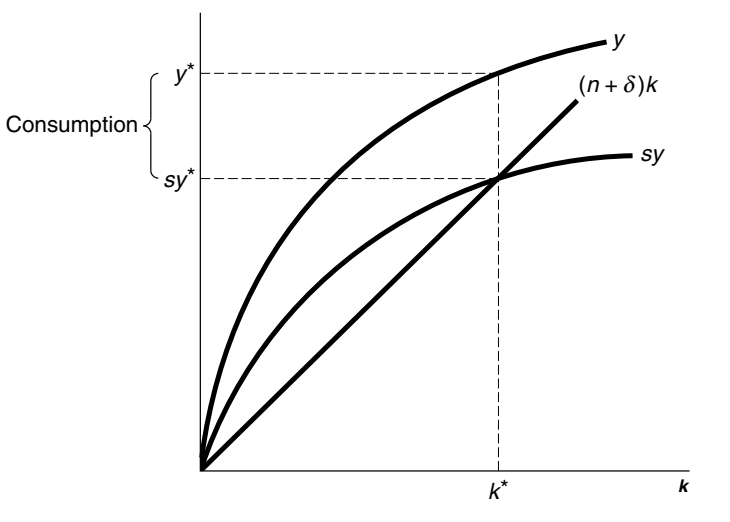
\includegraphics[width=0.75\linewidth]{Imagens/a5i1.png}
\end{figure}
\textbf{Observação}: às vezes chamamos \((n+\delta)\mathcal{k}\) de "requisito de investimento"


\subsection{\textbf{Estática comparativa} usando a equação 6}
Somente a exógena \( \mathcal{s} \) e a endógena \( \mathcal{k} \) variam.

Diferenciando \textbf{(6)} com respeito a \( \mathcal{s} \) e a \( \mathcal{k} \):

\[
d \mathcal{s} \cdot f(\mathcal{k}) + \mathcal{s} \cdot f'(\mathcal{k}) \cdot d\mathcal{k} = (\delta + n) \cdot d\mathcal{k}
\]

\[
\Rightarrow d \mathcal{s} \cdot f(\mathcal{k}) = d\mathcal{k} \left[ (\delta + n) - \mathcal{s} \cdot f'(\mathcal{k}) \right]
\]

\[
\Rightarrow \frac{d\mathcal{k}}{d\mathcal{s}} = \frac{f(\mathcal{k})}{[\ \cdot \ ]} = \frac{f(\mathcal{k})}{\mathcal{s} \left[ \frac{f(\mathcal{k})}{\mathcal{k}} - f'(\mathcal{k}) \right]}
\]

\[
= \frac{\mathcal{k} \cdot f(\mathcal{k})}{\mathcal{s} \left[ f(\mathcal{k}) - \mathcal{k} \cdot f'(\mathcal{k}) \right]} > 0
\]

Sabemos que a função \( f \) é \textbf{côncava}, então \( f(\mathcal{k}) - \mathcal{k} \cdot f'(\mathcal{k}) > 0 \), o que garante que a derivada seja positiva.

\textbf{Conclusão:} Como estamos lidando com o steady-state:

\[
\frac{d\mathcal{k}^*}{d\mathcal{s}} > 0 \Rightarrow \uparrow \mathcal{s} \Rightarrow \uparrow \mathcal{k}^* \Rightarrow \uparrow \hat{y}^*
\]

\begin{figure}[H]
    \centering
    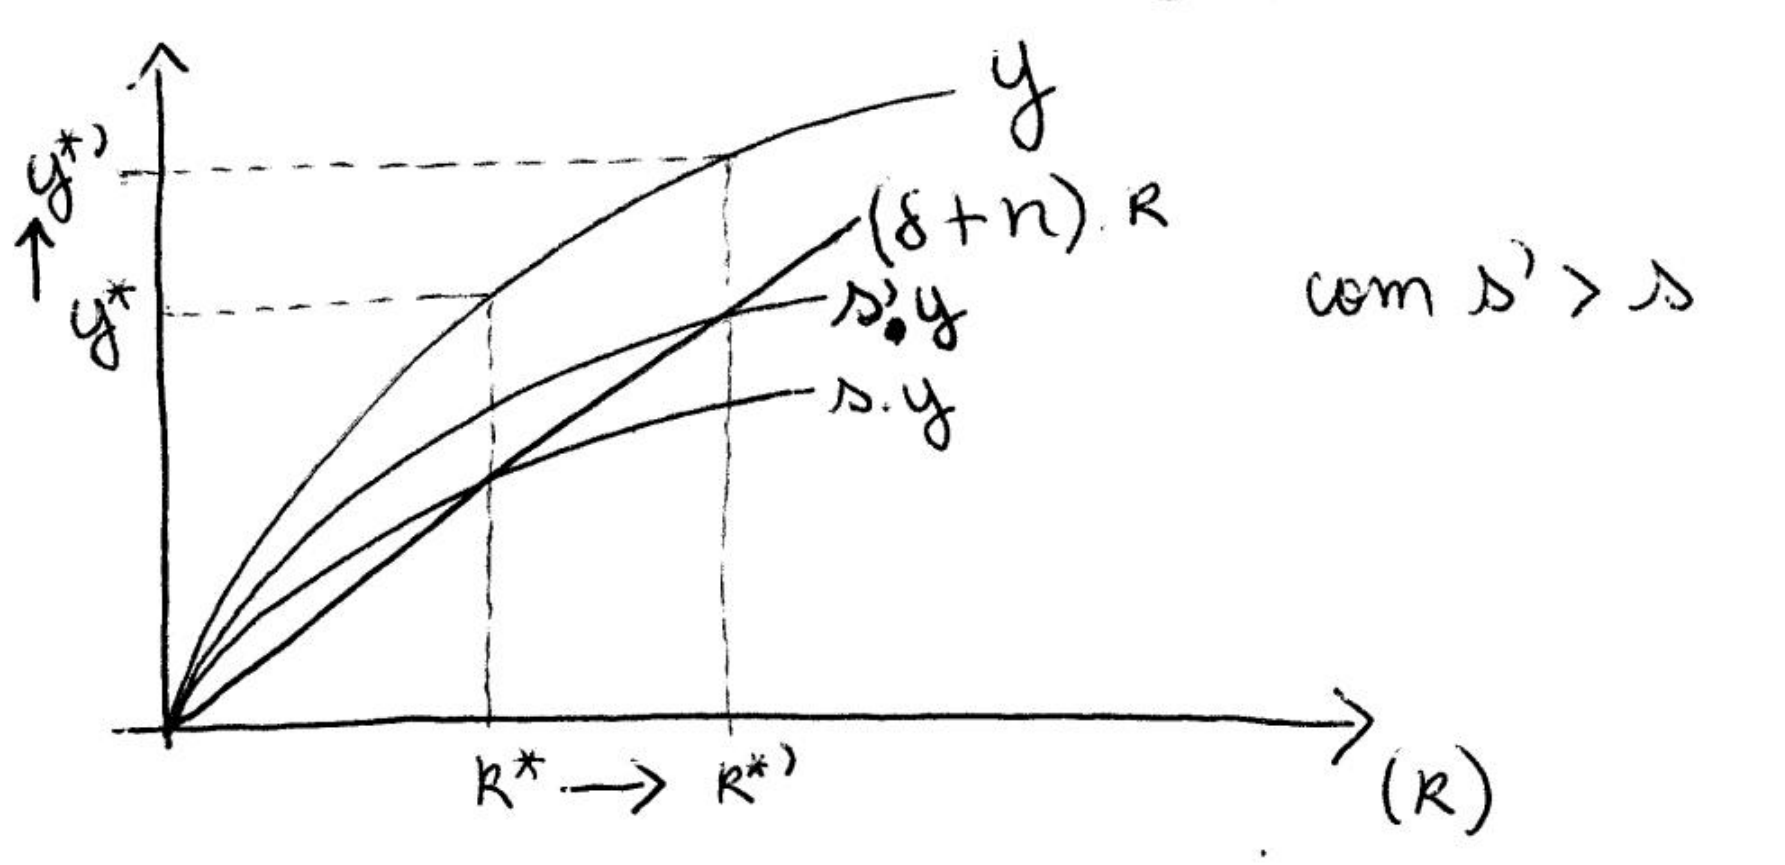
\includegraphics[width=0.7\linewidth]{Imagens/a7i1.png}
\end{figure}

\subsection{\textbf{2º Estática comparativa}}
Somente a exógena \( n \) e a endógena \( \mathcal{k} \) variam em

\[
\mathcal{s} f(\mathcal{k}) = \mathcal{k} \cdot (\delta + n) \tag{6}
\]

\[
\mathcal{s} f'(\mathcal{k}) d\mathcal{k} = (\delta + n) d\mathcal{k} + \mathcal{k} dn \Rightarrow
\]

\[
\Rightarrow \left[\mathcal{s} f'(\mathcal{k}) - (\delta + n)\right] d\mathcal{k} = \mathcal{k} dn
\]

\[
\Rightarrow \frac{d\mathcal{k}}{dn} = \frac{\mathcal{k}}{[\ \cdot \ ]} = \text{por (6)} = \frac{\mathcal{k}}{\mathcal{s} f'(\mathcal{k}) - \mathcal{s} \frac{f(\mathcal{k})}{\mathcal{k}}}
\]

\[
= \frac{\mathcal{k}/\mathcal{s}}{f'(\mathcal{k}) - \frac{f(\mathcal{k})}{\mathcal{k}}} = \frac{\mathcal{k}^2 / \mathcal{s}}{\mathcal{k} f'(\mathcal{k}) - f(\mathcal{k})} < 0
\]

\(< 0\) pois \( \mathcal{k} \) é côncava.

\[
\text{CONCLUSÃO:} \quad \frac{d\mathcal{k}^*}{dn} < 0, \quad \text{ou} \quad \uparrow n \Rightarrow \downarrow \mathcal{k}^* \Rightarrow \downarrow y^*
\]

\begin{figure}[H]
    \centering
    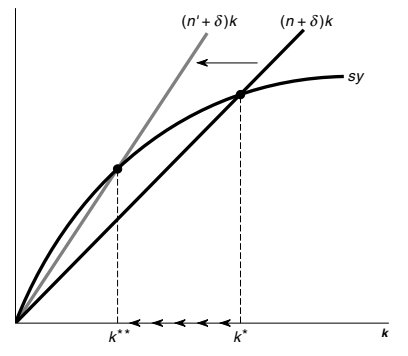
\includegraphics[width=0.7\linewidth]{Imagens/a7i2.png}
\end{figure}

Temos, então, 2 lições ou \textbf{\underline{predições}} importantes do modelo de \textbf{Solow}:

\begin{enumerate}
    \item\( \uparrow \mathcal{s} \rightarrow \uparrow y^* \), ou ``países que poupam mais têm maior produto per capita''
    \begin{figure}[H]
        \centering
        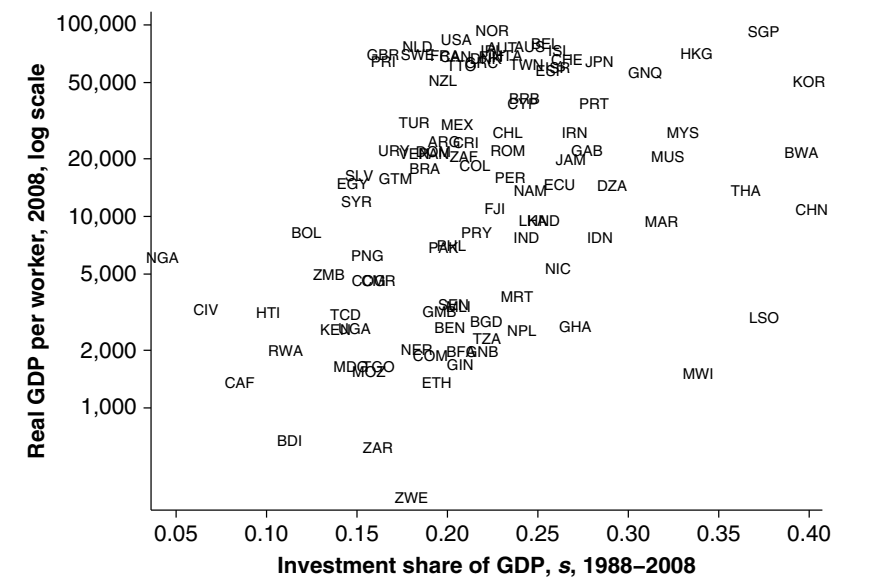
\includegraphics[width=0.7\linewidth]{Imagens/a7i3.png}
    \end{figure}
        
    \item\( \uparrow n \rightarrow \downarrow y^* \), ou ``países c/ maior crescimento populacional tendem a ser mais pobres''
    \begin{figure}[H]
        \centering
        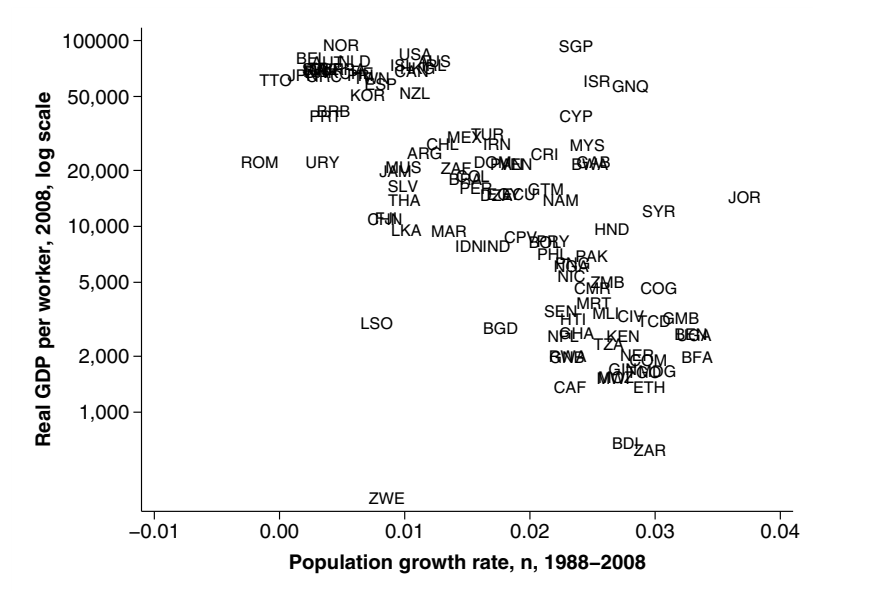
\includegraphics[width=0.7\linewidth]{Imagens/a7i4.png}
    \end{figure}
\end{enumerate}

\subsection{\textbf{EXERCÍCIO DE ``FIXAÇÃO''}}

Calcule (determine) o \( \mathcal{k}^* \) para o caso Cobb-Douglas, e faça os 2 exercícios de estática comparativa 
\(\left( \frac{d\mathcal{k}^*}{d\mathcal{s}} \text{ ou } \frac{dy^*}{d\mathcal{s}} \text{ e } \frac{d\mathcal{k}^*}{dn} \text{ ou } \frac{dy^*}{dn} \right)\) para esse caso.

\subsection{\textbf{Rendimentos decrescentes do capital e velocidade de convergência}}

Já vimos que:

\[
\dot{\mathcal{k}} = \mathcal{s} \cdot y - (\delta + n) \cdot \mathcal{k}
\]

onde \( y = f(\mathcal{k}) \).

Se \( F(K, L) = K^{\alpha} L^{1-\alpha} \), então:

\[
\frac{F(K, L)}{L} = F\left(\frac{K}{L}, 1\right) \equiv f(\mathcal{k}) = \left(\frac{K}{L}\right)^\alpha = \mathcal{k}^{\alpha}
\]

Então,

\[
\dot{\mathcal{k}} = \mathcal{s} \cdot \mathcal{k}^{\alpha} - (\delta + n) \cdot \mathcal{k}
\]

e a taxa de crescimento de \( \mathcal{k} \) é:

\[
\hat{\mathcal{k}} = \frac{\dot{\mathcal{k}}}{\mathcal{k}} = \mathcal{s} \cdot \mathcal{k}^{\alpha - 1} - (\delta + n) \quad \textbf{(7)}
\]

Como \( 0 < \alpha < 1 \), essa expressão é decrescente em \( \mathcal{k} \). Ou seja,

\[
q^{dg} \ll \mathcal{k} \ll \mathcal{k}^*
\]

\(\mathcal{k}\),resce rápido. Já que \( \mathcal{k} \) está quase atingindo \( \mathcal{k}^* \), ele cresce devagar. Em vista de (5), o mesmo vale para \( y \). Temos então que:

\[
\frac{d\hat{\mathcal{k}}}{d\mathcal{k}} < 0 \quad \text{e} \quad \frac{d\hat{y}}{dy} < 0 \ \ \textbf{(8)}
\]

Agora, isso pode ser interpretado de duas maneiras:

\begin{itemize}
    \item Um país tende a crescer mais rápido nos primeiros estágios do desenvolvimento.

    \item Dois países, \( i \) e \( j \), com tudo mais igual (\( s_i = s_j \), \( n_i = n_j \)), mas com \( y_i < y_j \), deverão crescer a taxas \( \hat{y}_i > \hat{y}_j \). Ou seja, há uma poderosa \textbf{força pró-convergência} no modelo de Solow!

\end{itemize}

Colocando de outra maneira, os países pobres podem crescer à mesma taxa que os EUA, mesmo com \( n \) ligeiramente maior que \( n_{\text{USA}} \) e \( s \) ligeiramente menor que \( s_{\text{USA}} \)... 

\textit{``So why can't these losers do their homework?''}

Representamos (7) e (8) através da...

\begin{figure}[H]
    \centering
    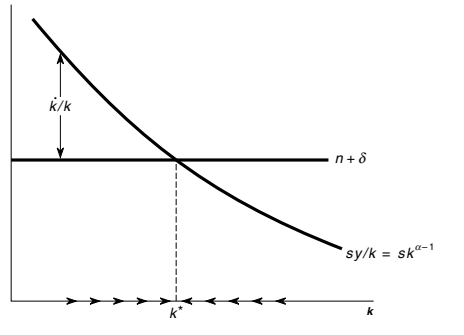
\includegraphics[width=0.5\linewidth]{Imagens/a7i5.png}
\end{figure}

\subsection{\textbf{Resumindo}}
No modelo simples de Solow (sem progresso tecnológico), \( \dot{\mathcal{k}} = 0 \) no steady-state \(\Rightarrow\)

\[
\frac{K}{L} \text{ e } \frac{Y}{L} \text{ constantes} \Rightarrow \hat{K} = \hat{Y} = \hat{L} = n
\]

mas \( \hat{y} = 0 \).


\(\Rightarrow\) \textit{contrafactual}: a maioria das economias experimenta crescimento sustentado de \( y \) (no longo prazo).

\underline{\textbf{progresso tecnológico no modelo de Solow}}:
\newpage

\section{\textbf{O Modelo de Solow- Com Progresso Tecnológico e Sem Capital Humano}}

No modelo de Solow, temos dois jeitos de incorporar a tecnologia:
\[
Y_t=F(K_t, A_tL_t)\rightarrow por \ exemplo = K^{\alpha}(A\cdot L)^{\alpha-1}
\]

Mas esse progresso tecnológico é gerado pelo o que(\textit{\textbf{Romer 1990}}) ? Mas quais as consequências do progresso tecnológico\textit{\textbf{Solow 1956,57}}? 

A variável tecnologia(nível tecnológico do país), \(A\), aparece associada ao fator trabalho \(L\). Especificação \textit{"Harrod-neutra"(Vamos usar essa especificação)} x \textit{"Hicks-neutra"}

\[
Y_t=\underbrace{A_t}_\text{TFP: Total Factors Productivity}\cdot F(K_t,L_t)
\]

Vamos usar a \(Y_t=K_t^{\alpha}(A_tL_t)^{1-\alpha}\) \textbf{(9)}

Progresso tecnológico \textbf{exógeno}(hipótese; modelo de Solow apenas supõem que o progresso tecnológico existe, ele não explica de onde ele vem):
\[
A_t=A_0\cdot e^{g_At} \Rightarrow \hat{A}\equiv\frac{\dot{A}}{A}\equiv \frac{\frac{dA}{dt}}{A}=g_a \ \ \textbf{(10)}
\]

Vamos definir \( \frac{X}{AL} \) como \( X \) por "trabalhador efetivo(AL)" ou por "unidade de eficiência de trabalho".

Usando a notação:
\[
x \equiv \frac{X}{L}, \quad \tilde{x} \equiv \frac{X}{AL} = \frac{x}{A}
\]

Então, usando \textbf{(9)}, temos:
\[
\tilde{y} = \left( \frac{K}{AL} \right)^{\alpha} = \tilde{\mathcal{k}}^{\alpha} \quad \textbf{(11)}
\]

Agora, definimos:
\[
\dot{\tilde{\mathcal{k}}} \equiv \frac{d\tilde{\mathcal{k}}}{dt} = \frac{\dot{K} \cdot AL - K \cdot \dot{(AL)}}{(AL)^2}
\]

\[
= \frac{\dot{K}}{AL} - \frac{K \cdot \dot{(AL)}}{AL^2} = \frac{\dot{K}}{AL} - \tilde{\mathcal{k}} \cdot \frac{\dot{A}L + A\dot{L}}{AL}
\]

\[
= \frac{\dot{K}}{AL} - \tilde{\mathcal{k}} \cdot \left( \frac{\dot{A}}{A} + \frac{\dot{L}}{L} \right)
\]

Pela equação \textbf{(3)}:

\[
= \frac{\mathcal{s}Y - \delta K}{AL} - \tilde{\mathcal{k}} \cdot \left( \frac{\dot{A}}{A} + \frac{\dot{L}}{L} \right)
\]

\[
= \mathcal{s} \cdot \tilde{y} - \delta \tilde{\mathcal{k}} - \tilde{\mathcal{k}} \cdot \left( \frac{\dot{A}}{A} + n \right)
\]

Usando \textbf{(10)}:

\[
= \underbrace{\mathcal{s} \cdot \tilde{y}}_\text{Construção} - \underbrace{\tilde{\mathcal{k}} \cdot (\delta + g_A + n)}_\text{Destruição}
\]

\[
= \underbrace{\mathcal{s} \cdot \tilde{\mathcal{k^\alpha}}}_\text{Construção} - \underbrace{\tilde{\mathcal{k}} \cdot (\delta + g_A + n)}_\text{Destruição}
\]

Finalmente, por \textbf{(11)}, temos que

\[
\textbf{(12)} \quad \dot{\mathcal{k}} = \mathcal{s} \cdot \tilde{\mathcal{k}}^{\alpha} - \tilde{\mathcal{k}} \cdot (\delta + g_A + n)
\]

Em steady-state, \( \dot{\mathcal{k}} = 0 \), portanto, por (12):

\[
\mathcal{s} \cdot \tilde{\mathcal{k}}^{\alpha} = \tilde{\mathcal{k}} \cdot (\delta + g_A + n)
\]

\[
\Rightarrow \quad \tilde{\mathcal{k}}^* \overbrace{\Rightarrow}^\text{Cobb-Douglas} \underbrace{\tilde{y}^* = \left( \frac{\mathcal{s}}{\delta + g_A + n} \right)^{\frac{1}{1-\alpha}}}_\text{cte} \quad \textbf{(13)}
\]

Por sua vez, por \textbf{(11)} e \textbf{(13)}, em uma Cobb-Douglas:

\[
\tilde{y}^* = (\tilde{\mathcal{k}}^*)^{\alpha} = \left( \frac{\mathcal{s}}{\delta + g_A + n} \right)^{\frac{\alpha}{1-\alpha}} ;\ \ \ \frac{\alpha}{1-\alpha}> 0 \quad \textbf{(14)}
\]

Então, é imediato ver que

\[
\frac{d\tilde{y}^*}{d\mathcal{s}} > 0, \quad \frac{d\tilde{y}^*}{d\delta} < 0, \quad \frac{d\tilde{y}^*}{dg_A} < 0, \quad \frac{d\tilde{y}^*}{dn} < 0
\]

Podemos representar a \textbf{(12)}:

\begin{figure}[H]
    \centering
    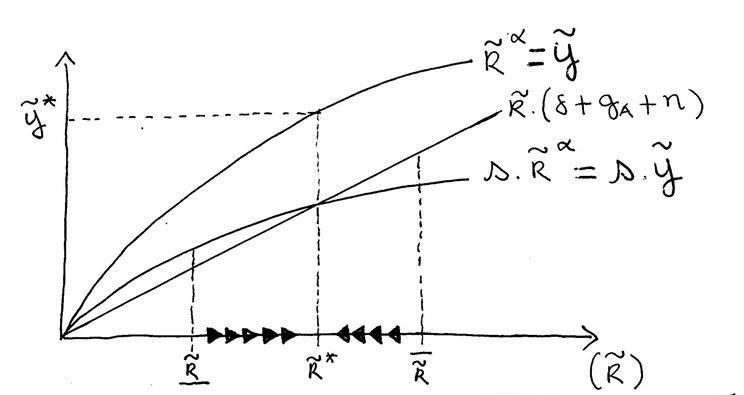
\includegraphics[width=0.7\linewidth]{Imagens/a10i1.png}
\end{figure}

Ora, \(\dot{\tilde{\mathcal{k}}} = 0\) \(\Rightarrow\) \(\dot{\tilde{y}} = 0\) \(\Rightarrow\) \(\frac{Y}{AL}\) constante \(\Rightarrow\)

\[
\hat{Y} = \underbrace{\hat{A} + \hat{L}}_{g_A + n}
\]

e 

\[
\hat{y} = \hat{A} \Rightarrow \underbrace{\hat{y} = {g_A}}_{\text{tx. de cresc. do prod. por trab. em steady-state}} \quad \textbf{(15)}
\]

Agora,

\[
\textbf{(14)} \Rightarrow \underbrace{y_t^*}_\text{cte ; Steady-Stae} = A_t \cdot \left( \frac{\mathcal{s}}{\delta + g_A + n} \right)^{\frac{\alpha}{1-\alpha}} \quad \textbf{(16)}
\]

Juntando isso com \textbf{(15)}, podemos dizer que um \(\uparrow \mathcal{s}\) ou \(\uparrow n\) afetam o nível do produto \textit{per capita} de steady-state, mas não sua taxa de crescimento. No Steady-State \(\tilde{y}=cte \rightarrow \frac{y}{A}\rightarrow \underbrace{g_y=g_a}_{g_y^*=g_a>0}\)

\textbf{obs.:} Podemos fazer em \textbf{(3)} o que fizemos para chegar a \textbf{(5)}, obtendo

\[
\hat{Y} = \alpha \cdot \hat{K} + (1-\alpha) \cdot \hat{L} + (1-\alpha) \cdot \hat{A}
\]

\[
\Rightarrow \text{por (15)} \Rightarrow g_A + n = \alpha \cdot \hat{K} + (1-\alpha) \cdot n + (1-\alpha) \cdot g_A
\]

\[
\Rightarrow \boxed{\hat{K} = \underbrace{n + g_A}_{\hat{Y}}} \quad \textbf{(17)}
\]

Ora, \textbf{(17)} implica que em steady-state (ou "balanced growth path") do modelo com tecnologia, a razão \textbf{\(\frac{K}{Y}\)} é constante... esse era um dos \textit{“fatos estilizados”} sobre a economia dos EUA que vimos na 1ª aula...

Por último, considere a "dinâmica transistória" de uma economia que estava no steady-state, com um certo \(\tilde{\mathcal{k}}^*\) e um certo \(\tilde{\dot{Y}}^*\), e daí sofre a "perturbação" (decorrente de uma política econômica, por ex.) $\uparrow \mathcal{s}$ :

\textbf{Por (14)}, sabemos que isso leva a \(\uparrow \tilde{y}^*\)... mas para haver \(\uparrow \tilde{Y}\), é preciso que durante algum tempo $Y$ cresça a uma taxa maior que a taxa de crescimento de $(A,L)$, ou que $y$ cresça a uma taxa maior que $g_A$ :

\begin{figure}[H]
    \centering
    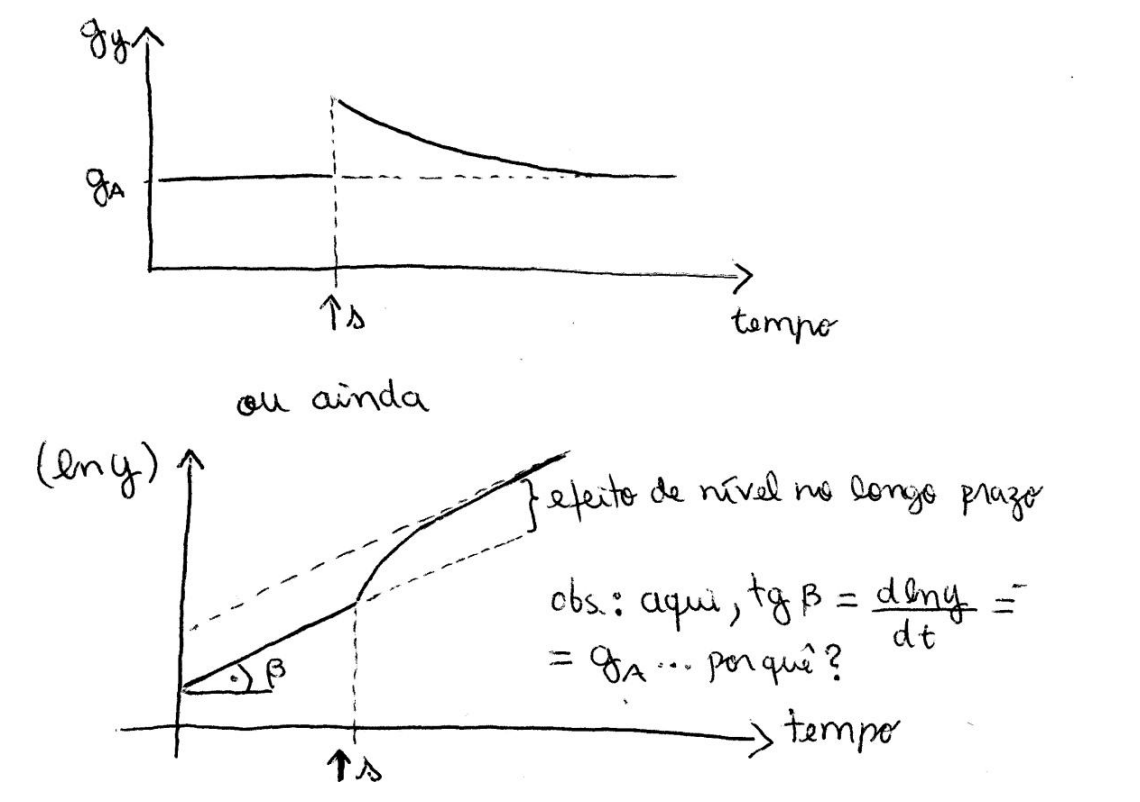
\includegraphics[width=0.7\linewidth]{Imagens/a12i1.png}
\end{figure}

O modelo de Solow com progresso tecnológico é importante porque o resultado \(\hat{y} \neq 0\) ou \(\hat{y} > 0\) é compatível com um fato estilizado sobre crescimento: observa-se crescimento sustentado na renda per capita dos países. No modelo simples, o crescimento não se sustentava porque \( f'(K) \) é decrescente (retornos decrescentes do \( \mathcal{K}^{\alpha L} \)). Agora, o progresso técnico compensa essa tendência do \( \mathcal{K}^{\alpha L} \).

Outro fato estilizado interessante: como explicar diferenças nas taxas de crescimento entre países? \(\rightarrow\) dinâmica de transição \(\rightarrow\) países próximos do steady-state (EUA, por ex.) crescem mais devagar do que países longe do s-s (Brasil, por ex.), se pensarmos numa média para o século XX. Além disso, transitoriamente, \(\uparrow S \rightarrow \uparrow \hat{Y}\), o que se aplica aos "tigres asiáticos", como a Coreia do Sul a partir de 1950.

\(...\) \textbf{Rumo ao crescimento endógeno}: nos modelos de crescimento exógeno (variações do modelo de Solow que acabamos de ver), nem \(\hat{y}\) nem \(\hat{c}\) nem \(\hat{R}\) do steady-state são afetados por \( S \) (variável de política).

\newpage
\section{\textbf{Avaliação de Solow 1}}
\subsection{\textbf{Avaliação do Modelo de Solow}}

Como vimos, um \( \uparrow \mathcal{s} \) (ou \( \uparrow \) tx. de investimento) leva, transitoriamente, a um crescimento de \( y \) a uma tx. superior à de steady-state (\( g_A \)). Os países do Leste Asiático cresceram a txs. em torno de \( 5\% \gg 2\% (g_A) \) a partir de 1950. Terão eles elevado suas txs. de poupança nesse período?

Jones, figura 2.14 \(\rightarrow\) \text{exceção: Hong Kong}. 

\begin{figure}[H]
    \centering
    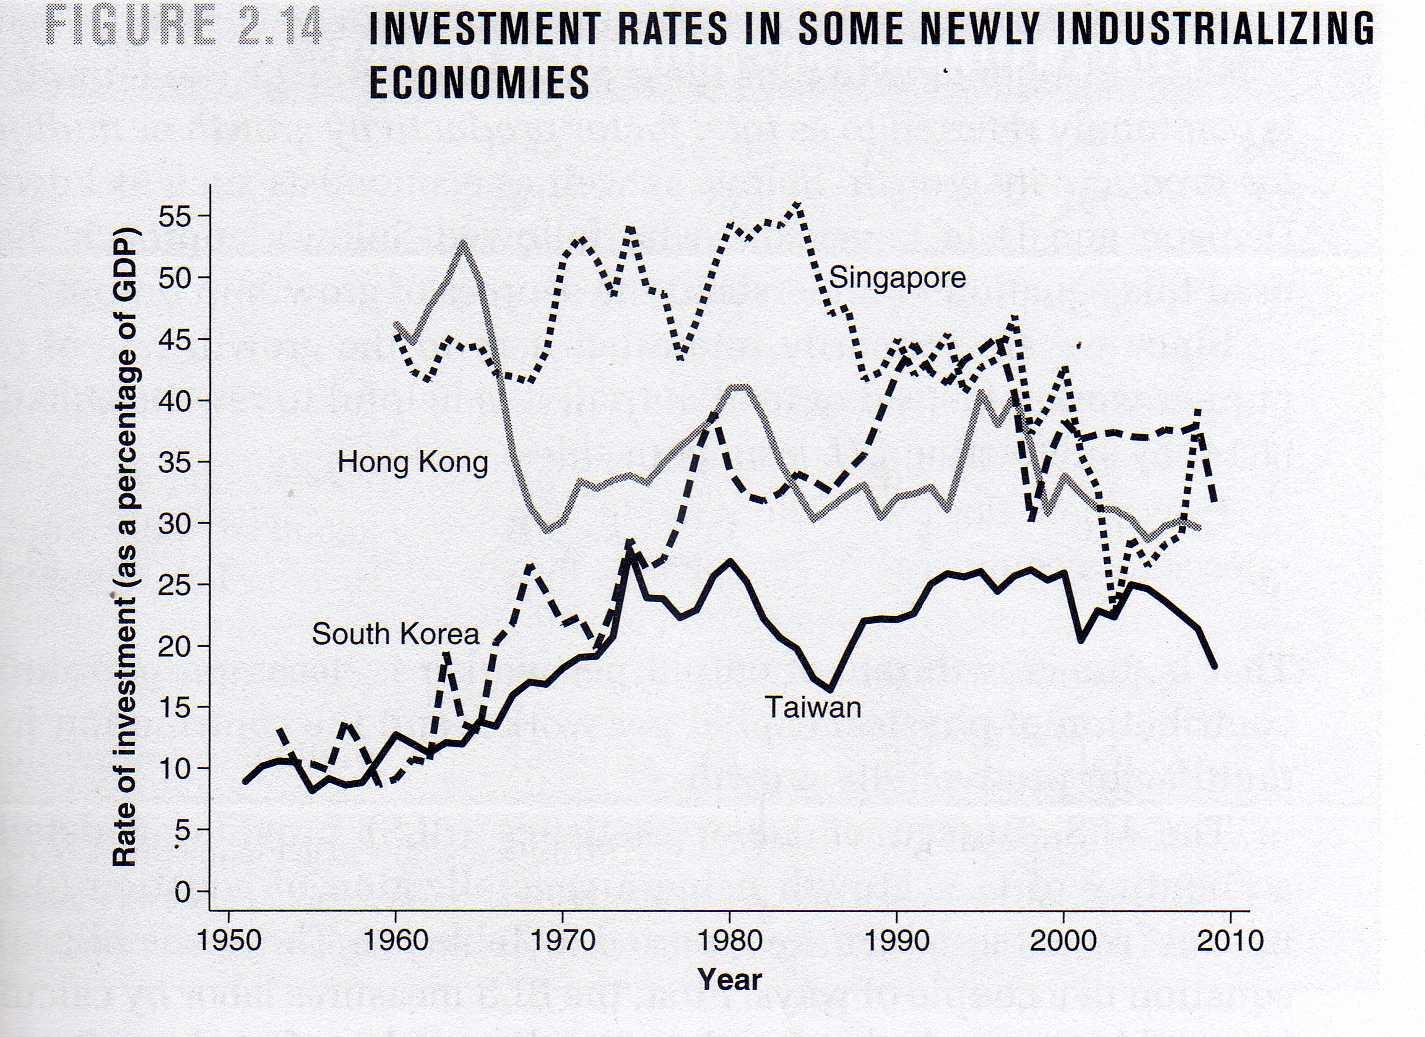
\includegraphics[width=0.7\linewidth]{Imagens/a12i2.png}
\end{figure}

O crescimento não é bem explicado pelo modelo de Solow (acumulação de capital).

\subsubsection{\textbf{Decomposição do Crescimento (Solow, 1957)}}

\[
Y = B \cdot K^{\alpha} \cdot L^{1-\alpha} \quad \text{(especificação Hicks-neutra)}
\]

\[
\Rightarrow \text{tomando a especificação Harrod-neutra, i.e., } Y = K^\alpha \cdot (A \cdot L)^{1-\alpha}, \text{ segue-se que } B = A^{1-\alpha}
\]

\[
\Rightarrow g_B \equiv \frac{\dot{B}}{B} = (1-\alpha) \cdot g_A
\]

\subsubsection{\textbf{Considerando a especificação Hicks-neutra, podemos decompor:}}

\[
\frac{\dot{Y}}{Y} = \frac{\dot{B}}{B} + \alpha \cdot \frac{\dot{K}}{K} + (1-\alpha) \cdot \frac{\dot{L}}{L}
\]

Podemos observar/medir "diretamente" \( \frac{\dot{Y}}{Y} \), \( \frac{\dot{K}}{K} \) e \( \frac{\dot{L}}{L} \).

Daí que \( \frac{\dot{B}}{B} \) seja calculado como um \textbf{RESÍDUO (de Solow)}.

Sua interpretação é: que parte do crescimento do PIB não pode ser atribuída à acumulação de fatores, devendo, mensuravelmente, ser atribuída ao progresso tecnológico ou TFP (Total Factors' Productivity).

\subsection{\textbf{Exemplos ou casos interessantes}}

\begin{itemize}
    \item \textbf{1º} \( \downarrow \) na taxa de crescimento de \( y \) nos EUA a partir de 1970: quadro 2.1 Jones.
    \item \textbf{2º} Qual a causa do alto \( g_Y \) dos países do Leste Asiático? Acumulação de fatores ou TFP? (figura 2.15 Jones)
\end{itemize}

\textbf{Jones:} 
\begin{itemize}
    \item Obs.: onde se situam os EUA, economia em steady-state? E a Coreia?
\end{itemize}

\subsection{\textbf{Aplicações empíricas dos modelos de crescimento neoclássicos (Jones, cap. 3 + comentários do prof.)}}

Num \textit{paper} seminal, Mankiw, Romer (David, não Paul) e Weil (MRW 1992, daqui p/ frente) procuraram usar o modelo de Solow p/ explicar diferenças internacionais de renda \textit{per capita}.

Numa primeira tentativa, em que as únicas fontes de variabilidade internacional eram \( n \) (tx. de crescimento populacional) e \( \mathcal{s}_K \) (tx. de poupança ou investimento em capital físico), a qualidade de ajuste do modelo de regressão foi \( R^2 = 0,59 \) — mas, impondo a restrição de que o parâmetro \( \alpha \) em

\[
Y = K^\alpha \cdot (A \cdot L)^{1-\alpha}
\]

tem que ser igual à participação do capital na renda (ou seja, \( \alpha = \frac{1}{3} \)), o ajuste caiu para \( R^2 = 0,28 \).

Diante disso, MRW (1992) incorporaram \textbf{capital humano} ao modelo básico de Solow — afinal, essa é um fator acumulável em que os países apresentam considerável variabilidade.

Vale a pena destacar algumas das \textbf{hipóteses} usadas no modelo de Solow com capital humano de MRW (1992):

\begin{itemize}
    \item\textbf{Todas as economias (países) estão em steady-state}: 
    Se o tempo que uma economia leva para atingir ou chegar, digamos, 95\% perto do steady-state for curto, então essa é uma hipótese razoável para a análise de longo prazo.
    
    \item \textbf{Tecnologias idênticas internacionalmente}: 
    \[
    A_{it} = A_{jt}, \quad \forall  \ \ t \text{ e os países } i, j
    \]
    (Essa é uma hipótese honesta, caso se pretenda testar o modelo de Solow, em que o progresso tecnológico não é explicado pelo modelo.)
    
    \item \textbf{O capital humano é acumulado da mesma maneira que o capital físico}: 
    \[
    \underbrace{\dot{H}}_{\text{Variação no estoque de capital humano}} = 
    \underbrace{s_H \cdot Y}_{\text{taxa de investimento em capital humano}} - 
    \delta_H \cdot H
    \]
    \item Variação no estoque de capital humano: Essa hipótese foi duramente criticada, por exemplo, por Klenow e Rodriguez (1997), e por esse motivo...
\end{itemize}

Jones decide seguir Lucas (1988) e Bils e Klenow (1996) supondo que as pessoas gastam tempo acumulando capital humano (qualificações) ao invés de trabalhar (produzir "bens finais").

Ainda assim, vale a pena lembrar que o modelo com capital humano de MRW (1992) apresenta uma boa qualidade de ajuste (\( R^2 = 0,78 \))...

\subsection{\textbf{Modelo de Solow com Capital Humano – Versão Jones}}

\[
Y = K^\alpha \cdot (A \cdot H)^{1-\alpha} \quad \textbf{(1)}
\]

\textbf{Capital humano}
\[
H = e^{\psi \cdot u} \cdot L_Y \quad \textbf{(2)}, \quad \psi > 0
\]

Dado \(\psi\) definido como : retorno da educação (ex: quantos \% de aumento salários para cada ano adicional de estudo. E \(L_y\) definido como quantidade de trabalho alocada para produzir bens finais.

\textbf{Quantidade de trabalho alocada para produzir bens finais.}

\[
L_Y = (1 - u) \cdot L \quad \textbf{(3)}
\]

Sendo \(u\) definido como : fração do tempo que o trabalhador médio gasta adquirindo habilidades (qualificação). E \(L\) força de trabalho.

\textbf{Observações:} 
\begin{itemize}
    \item Pela equação (3), se \( u = 0 \), então \( L_Y \) é máximo, i.e., \( L_Y = L \).
    \item Pela equação (2), se \( H = L_Y \), implica em, toda a força de trabalho é não-qualificada.
\end{itemize}

\textbf{Observação:} Pela equação (2),

\[
\Rightarrow \frac{dH}{du} = H \cdot \psi \Rightarrow \frac{dH/du}{H} = \psi
\]

o que significa que quando \( u \) aumenta infinitesimalmente, \( H \) cresce \( \psi \cdot 100\% \). Em outras palavras, o aumento em \( H \) é proporcional a \( H \)... "Essa formulação procura levar em conta parte substancial da literatura de economia do trabalho que considera que cada ano adicional de escolaridade aumenta o salário ganho por uma pessoa em algo em torno de 10\%."

Como poderíamos então calibrar \(\psi\) ??

\[
\dot{K} = s_k \cdot Y - \delta \cdot K \quad (4)
\]

A seguir, dividindo (1) por \(L_y\), vem

\[
y = K^{\alpha} \cdot (A \cdot h)^{1-\alpha}
\]

onde, por (2), \( h = e^{\psi \cdot u} \).

Observação: \( u \) é exógena e constante \(\Rightarrow h\) é constante. Vamos trabalhar com variáveis estacionárias do tipo:

\[
\tilde{X} \equiv \frac{X}{(L_y \cdot A \cdot h)}
\]

Assim, ficamos com:

\[
y = K^{\alpha} \cdot (A h)^{1-\alpha} \quad (5)
\]

ou

\[
\tilde{y} = \tilde{\mathcal{k}}^{\alpha} \quad (6)
\]

, nossa velha conhecida.

Levando em conta (4) e a definição de variável estacionária (\(\tilde{x}\) acima), vem

\[
\dot{\tilde{\mathcal{k}}} = \mathcal{s}_k \cdot \tilde{y} - (n + g_A + \delta) \cdot \tilde{\mathcal{k}} \quad (7)
\]

...enfim, acrescentou-se o capital humano sem alterar a estrutura do modelo. Fazendo \(\dot{\tilde{\mathcal{k}}} = 0\), no steady-state, e substituindo (6), vem

\[
\tilde{y}^* = \left(\frac{\mathcal{s}_k}{n+g_A+\delta}\right)^{\frac{\alpha}{1-\alpha}} \quad (8)
\]

Reescrevendo (8) em termos de produto por trabalhador, temos

\[
\underbrace{y^*(t)}_\text{Variáveis que crescem ao longo do tempo} = \left(\frac{\mathcal{s}_k}{n+g_A+\delta}\right)^{\frac{\alpha}{1-\alpha}} \cdot h \cdot \underbrace{A(t)}_\text{Variáveis que crescem ao longo do tempo} \quad (8')
\]



Agora, seria interessante, em (8'), discutir que variáveis/parâmetros são "country-specific", implica em, podem variar de país para país... Consideremos o produto por trabalhador do país \( i \), em relação ao dos USA, em steady-state:

\[
\frac{y_i^*(t)}{y_{USA}^*(t)} =
\frac{\left(\frac{s_{k_i}}{n_i + g_{A_i} + \delta} \right)^{\frac{\alpha}{1-\alpha}} \cdot h_i \cdot A_i(t)}
{\left(\frac{s_{k_{USA}}}{n_{USA} + g_{A_{USA}} + \delta} \right)^{\frac{\alpha}{1-\alpha}} \cdot h_{USA} \cdot A_{USA}(t)}
\quad (9)
\]

Note que, se supomos \( g_{A_i} \neq g_{A_{USA}} \), então \( y_i^*/y_{USA}^* \) não será constante ao longo do tempo! Para que as rendas per capita relativas sejam constantes ao longo do tempo (em steady-state), vamos assumir \( g_{A_i} = g_{A_{USA}} = g_A \). Note que isso não implica supor \( A_i = A_{USA} \). Com isso, temos que as diferenças internacionais de \( y_i \) são explicadas por diferenças de \( n_i \), de \( s_{k_i} \) e de \( u_i (h_i) \).

\[
\vdots
\]

\textbf{Ajustamento do modelo:}

\begin{itemize}
    \item \textbf{1º exercício}: assumindo \( A_i = A_{USA} \); \( \alpha = \frac{1}{3} \); \( \psi = 0,10 \) (cada ano extra de escolaridade aumenta em 10\% o salário do trabalhador);
    \item \( u_i = \) anos de escolaridade (média do país \( i \));
    \item \( g_A + \delta = 0,075 \);
    \item E por (9) estimamos
\end{itemize}

\[
\frac{y_i^*(t)}{y_{USA}^*(t)} \quad \text{previsto pelo modelo} \quad \longrightarrow \quad \text{comparar com} \quad \frac{y_i^*(t)}{y_{USA}^*(t)} \quad \text{observada}
\]

Note que:

\begin{itemize}
    \item Para os países ricos, há boa qualidade do ajustamento (aderência à linha de 45º).
    \item Para os países pobres:
\end{itemize}

\[
\frac{y_i}{y_{USA}}_{\text{previsto}} > \frac{y_i}{y_{USA}}_{\text{observado}}
\]

\textbf{2º exercício}: assumindo \( A_i \neq A_{USA} \)

\begin{itemize}
    \item Usando (5), podemos estimar \( A_i \):
\end{itemize}

\[
y_i = \mathcal{K}_i^\alpha \cdot (A_i \cdot h_i)^{1-\alpha}
\]

\[
\Rightarrow A_i = \left(\frac{y_i}{\mathcal{K}_i}\right)^{\frac{\alpha}{1-\alpha}} \cdot \frac{y_i}{h_i} \quad (5')
\]

Onde \( \frac{y_i}{\mathcal{K}_i} \) é o inverso da relação capital/produto, algo "observável".

Incorporando (5') em (9) e fazendo novamente:

\[
\frac{y_i^*(t)}{y_{USA}^*(t)}_{\text{previsto}} \quad \longrightarrow \quad \frac{y_i^*(t)}{y_{USA}^*(t)}_{\text{observado}}
\]

A qualidade do ajustamento parece incrível, mas...

\textbf{Algumas críticas:}

Uma observação mais atenta das estimativas de \( A \) revela algo interessante: embora os níveis de \( A \) estejam altamente correlacionados com os níveis de renda, a correlação não é perfeita. Notadamente, países como França e Hong Kong têm estimativas muito altas de \( A \). 

Isso nos leva a uma afirmação importante: estimativas de \( A \) calculadas dessa maneira são como resíduos da decomposição do crescimento, incorporando quase que inteiramente diferenças na produção não explicadas pelos insumos. Por exemplo, não temos controle sobre as diferenças de qualidade dos sistemas educacionais dos diferentes países, de modo que essas diferenças estarão incluídas em \( A \). 

Nesse sentido, pareceria mais adequado referir-se a essas estimativas como níveis de produtividade total dos fatores do que como níveis tecnológicos.

O que Jones candidamente deixa de dizer (como um bom defensor do modelo neoclássico de crescimento) é que, em vez de (5'), poderíamos "estimar" \( A_i \) de modo que:

\[
\frac{y_i}{y_{USA}}_{\text{previsto}} = \frac{y_i}{y_{USA}}_{\text{observado}}
\]

Ou seja, o modelo perderia todos os graus de liberdade para um teste empírico!

\newpage
\section{\textbf{Avaliação Solow 2}}

\subsection{\textbf{Convergência e explicação das diferenças nas taxas de crescimento}}

\begin{itemize}
    \item Por que deveria haver convergência? Autores como Gerschenkron (1952) 
    e Abramovitz (1986) destacam a \emph{advantage of backwardness} 
    (ligada ao \emph{fishing out effect}): 
    \begin{itemize}
        \item Para países na fronteira tecnológica, cada novo avanço é mais difícil.
        \item Para países longe da fronteira, seria mais fácil adotar ou adaptar 
              tecnologias já existentes.
    \end{itemize}
    \item Em termos do modelo de Solow, mesmo para economias ou países isolados, 
    prevalecem os rendimentos decrescentes do capital, o que sugere convergência 
    (se houver mecanismos que permitam acumular capital até certo ponto).
    \item Quando falamos de convergência, subentende-se que, se 
    \[
      y_i < y_j \quad \Longrightarrow \quad g_{y_i} > g_{y_j},
    \]
    ou seja, os países mais pobres fazem um \emph{catch up} (terminologia de Abramovitz).
\end{itemize}

Evidência histórica (Baumol, 1986):
\begin{itemize}
    \item Figuras 3.3 de Jones mostram trajetórias dos PIBs per capita 
    (em escala log) de 4 países a partir de 1870.
    \item Figuras 3.4, 3.5 e 3.6 de Jones: \emph{plot} de taxas anuais médias de 
    crescimento versus PIB per capita inicial.
    \item Isso sugere uma primeira especificação para \emph{growth regressions}:
    \[
      g_{y_i}(t_0 \to t_n) \;=\; \beta_0 \;+\; \beta_1 \, y_{i,t_0} \;+\; \varepsilon_i,
    \]
    onde a convergência implicaria \(\beta_1 < 0\).
    \item Conclusões preliminares:
    \begin{itemize}
        \item Das Figuras 3.4 e 3.5 (países ``ricos'' ou desenvolvidos) 
              parece haver convergência.
        \item Da Figura 3.6, ao se acrescentar países ``pobres'' ou em desenvolvimento, 
              a qualidade do ajuste dessas regressões de crescimento cai bastante. 
              Em geral, não se observa convergência mundial.
    \end{itemize}
\end{itemize}

\subsection{\textbf{Convergência condicional}}

\begin{itemize}
    \item Pergunta: 
    \emph{``Por que, então, vemos convergência entre alguns conjuntos de países, 
    mas não convergência entre todos os países do mundo?''}

    \item Outra questão: 
    \emph{``Um país deve necessariamente crescer mais rápido só porque é mais pobre?''} 
    Resposta: não. Isso remete à ideia de convergência condicional.
\end{itemize}

Para entender isso, devemos considerar que muitas vezes olhamos para variáveis do tipo 
\[
  \tilde{x} \;=\; \frac{X}{A\,L_y\,h}
  \quad\Longrightarrow\quad
  \frac{x_c}{A\,h},
\]
nas dinâmicas de transição. Países \(i\) e \(j\) podem ter \(h_i \neq h_j\) 
(ou seja, produtividade do trabalho ou escolaridade diferentes) e, portanto, \(u_i \neq u_j\); 
mas vamos supor essas variáveis constantes ao longo do tempo, de modo que isso não afete 
a taxa de crescimento desses países. Quanto a \(A\), vamos admitir \(A_i \neq A_j\), 
mas \(\dot{A}_i = \dot{A}_j = \text{const}\); de modo que variações em \(\hat{y}_i\) 
e \(\hat{\mathcal{k}}_i\) ao longo do tempo reflitam principalmente a dinâmica de acumulação de capital 
(modelo de Solow).

Recordando que
\[
  \hat{y} \;=\; \alpha \,\hat{\mathcal{k}},
  \quad
  \hat{\mathcal{k}} \;=\; \mathcal{s}_R \,\frac{\dot{K}}{K}
  \;=\; \mathcal{s}_R \,\frac{\dot{\tilde{\mathcal{k}}}}{\tilde{\mathcal{k}}}
  \;-\; (\delta + n + g_A),
\]
para o caso Cobb-Douglas:
\(\frac{\dot{\tilde{\mathcal{k}}}}{\tilde{\mathcal{k}}} = g_{\tilde{\mathcal{k}}}= \underbrace{\mathcal{s}_K \,\tilde{\mathcal{k}}^{\,\alpha-1}}_\text{construção} - \underbrace{(\delta + n + g_A)}_\text{destruição}\), etc. 
Isso mostra que \(\hat{\mathcal{k}}\) é decrescente em \(\tilde{\mathcal{k}}\), e \(\hat{y}\) é decrescente 
em \(\tilde{y}\).

\subsection{\textbf{Dinâmicas de transição para países com estados estacionários diferentes}}

\begin{figure}[H]
    \centering
    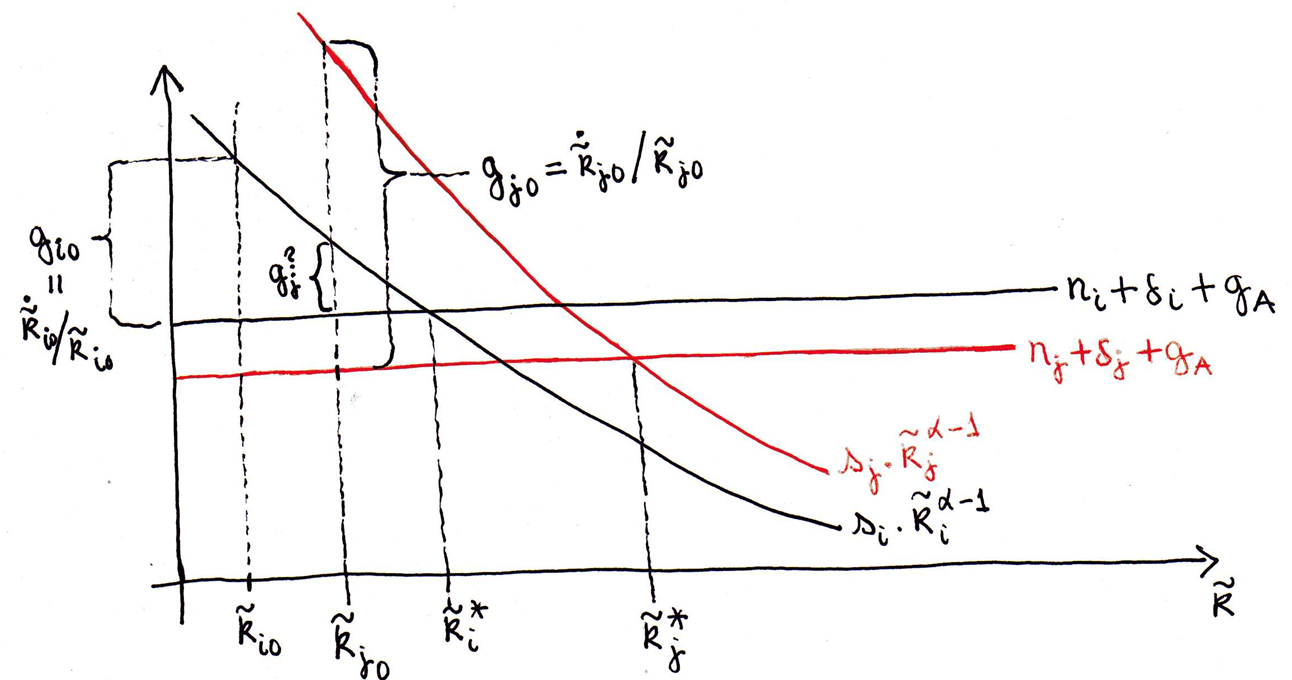
\includegraphics[width=0.7\linewidth]{Imagens/a13i1.png}
\end{figure}

\begin{itemize}
    \item No diagrama (como em Jones, Figura 3.8), países que têm \(\tilde{\mathcal{k}}_{j,0}\) 
    maior do que \(\tilde{\mathcal{k}}_{i,0}\) não necessariamente crescem mais devagar 
    se seus parâmetros \((\mathcal{s}_i, n_i, g_{A,i})\) diferem.
    \item Uma explicação visual:
    \begin{itemize}
        \item Se olharmos para distâncias verticais, poderíamos supor 
        \(\tilde{\mathcal{k}}^{\,\alpha -1} - (\delta + n + g_A)\). 
        \item Mas, se olharmos para distâncias \emph{horizontais} em relação ao 
        estado estacionário \(\tilde{\mathcal{k}}^*\), vemos que, se \(\tilde{\mathcal{k}}_{j,0}\) 
        está acima de \(\tilde{\mathcal{k}}_{i,0}\) mas ainda \(\tilde{\mathcal{k}}_{j,0} < \tilde{\mathcal{k}}_{j}^*\), 
        esse país pode crescer até alcançar seu estado estacionário. 
        \item Assim, surge a ideia de convergência condicional no modelo de Solow.
    \end{itemize}
\end{itemize}

Comparando as Figuras 3.6 e 3.8 de Jones:
\begin{itemize}
    \item Embora países mais pobres não cresçam necessariamente a uma taxa maior, 
    os países que são \emph{pobres} em relação ao seu próprio estado estacionário 
    tendem a crescer mais rápido. 
    \item Exemplos (em 1960) incluíram Coreia, Japão, Cingapura e Hong Kong, 
    que se mostraram relativamente pobres em relação ao seu \emph{steady-state} 
    e, por isso, apresentaram taxas de crescimento elevadas.
\end{itemize}

\subsection{\textbf{Resumo}}

\begin{itemize}
    \item Convergência absoluta: se dois países têm os mesmos parâmetros 
    \(\mathcal{s}_K, n, \dots\), então
    \[
      y_i < y_j \;\;\Longrightarrow\;\; g_{y_i} > g_{y_j}
      \quad\Longrightarrow\quad
      y_i \to y_j \;\text{ ao longo do tempo.}
    \]
    \item Convergência condicional: cada país (ou \emph{grupo de convergência}) 
    tende ao seu próprio estado estacionário. Nesse caso,
    \[
      (y_i - y_i^*) \;\to\; 0 
      \quad \text{e} \quad
      (y_j - y_j^*) \;\to\; 0,
    \]
    desde que \(y_i^*\) e \(y_j^*\) sejam diferentes, mas determinados por 
    fundamentos como \(\mathcal{s}_K, n, g_A\).
    \item Ideia de \emph{clubes de convergência}: países que compartilham 
    parâmetros semelhantes (\(\mathcal{s}_K, n, g_A\)) tendem a convergir entre si.
\end{itemize}

\subsection{\textbf{Por que países estariam fora do seu estado estacionário?}}

\begin{itemize}
    \item Nossa explicação das diferenças de taxas de crescimento (convergência condicional) 
    foi baseada na dinâmica de transição. Então, por que estariam fora do steady-state?
    \item Possíveis razões:
    \begin{itemize}
        \item Destruição de estoques de capital (ex.: Segunda Guerra Mundial).
        \item Aumento da taxa de poupança em países do Leste Asiático após 1950--60.
        \item Deterioração das condições macroeconômicas (hiperinflação na 
              América Latina nos anos 80) levando a queda de poupança e investimento.
    \end{itemize}
\end{itemize}

\subsection{\textbf{A evolução da distribuição internacional de renda (tópico 3.3)}}

\begin{itemize}
    \item Algumas medidas:
    \begin{enumerate}
        \item Evolução da renda per capita relativa dos países 5\% mais ricos 
              versus 5\% mais pobres (Figura 3.9 de Jones). 
              Conclusão: não houve convergência absoluta; 
              talvez até pequena divergência.
        \item Observando apenas os extremos (5\% mais pobres e 5\% mais ricos) 
              e comparando a distribuição em três períodos (1960, 1990 e 
              um \emph{steady-state} projetado -- Figura 3.10 de Jones), 
              pergunta-se: \emph{como interpretar?}
              \begin{itemize}
                  \item Para percentis intermediários (40\%, 50\%, 60\%) e superiores (70\%), 
                        \(\frac{y_{1990,i}}{y_{1990,\text{USA}}} 
                          > 
                          \frac{y_{1960,i}}{y_{1960,\text{USA}}}\), 
                        indicando convergência.
                  \item Mas para percentis inferiores, o sinal inverte-se, 
                        sugerindo divergência.
              \end{itemize}
    \end{enumerate}
    \item Sobre a Figura 3.10: projeções para o futuro (steady-state). 
    \begin{itemize}
        \item Os EUA perderão sua liderança? Revisando o Quadro 3.1, 
              um ponto forte dos EUA é a alta taxa de investimento em capital humano 
              (alta escolaridade), mas um ponto fraco é a baixa taxa de poupança 
              e investimento em capital físico.
        \item É razoável assumir que, no longo prazo, entre países desenvolvidos, 
              haja convergência de níveis de produtividade.
    \end{itemize}
\end{itemize}


\newpage
\section{\textbf{Romer 1}}

\subsection{\textbf{Apontamentos sobre Crescimento Endógeno}}
\begin{itemize}
    \item Uma das motivações dos primeiros modelos de crescimento endógeno 
    é fazer com que a taxa de crescimento de longo prazo (LP) 
    dependa de variáveis de política, como gastos públicos em pesquisa básica.

    \item Referências clássicas:
    \begin{itemize}
        \item Romer (1986, 1990)
        \item Aghion e Howitt (1992)
        \item Grossman e Helpman (1991)
    \end{itemize}

    \item Nos modelos de crescimento endógeno, o progresso técnico é resultado 
    de atividade intencional (visando lucro) de P\&D por parte das empresas.
\end{itemize}


\subsection{\textbf{A Economia das Ideias}}
\begin{itemize}
    \item Ideias (invenções, designs de novos produtos, novos processos) possuem:
          \begin{itemize}
              \item Ausência de rivalidade: o uso por 1 agente não exclui nem reduz o uso por outros.
              \item Dessa ausência de rivalidade decorrem retornos crescentes.
          \end{itemize}

    \item Exemplo de função de produção (hipotética) para ilustrar:
    \[
      Y = 1000 \cdot (L - 800),
    \]
    onde:
    \begin{itemize}
      \item $L$ é o total de trabalhadores.
      \item 800 é o custo (em unidades de trabalho) para inventar (fixo) um novo software.
      \item Produzir uma cópia adicional custa 
            $\tfrac{1}{1000}$ unidade de trabalho por cópia.
    \end{itemize}

    \item Interpretação:
    \begin{itemize}
      \item O produto final pode ser CD contendo 1 novo software.
      \item Os 800 trabalhadores são empregados (fixos) para a invenção inicial.
      \item Cada cópia adicional do software exige $\frac{1}{1000}$ de trabalhador.
    \end{itemize}
\end{itemize}


\subsection{\textbf{Custos e concorrência imperfeita}}
\begin{itemize}
    \item A função custo correspondente para $Y$ é:
    \[
      C(Y) = 800\,W + \frac{W}{1000}\,Y,
    \]
    onde $W$ é o salário.
    \begin{itemize}
      \item $800\,W$ é o custo fixo.
      \item $\frac{W}{1000}\,Y$ é o custo variável (custo marginal)\(CM_g\).
    \end{itemize}

    \item Assim, o Custo Médio (CMe) e o Custo Marginal \(CMg\) são:
    \[
      \text{CMe} = \frac{800\,W}{Y} + \frac{W}{1000},
      \quad
      \text{CMg} = \frac{W}{1000}.
    \]

    \item Observa-se que:
    \begin{itemize}
        \item O CMe é decrescente em $Y$.
        \item Em concorrência perfeita, o preço $P$ tenderia a se igualar a $CMg$. 
              Mas se $P = CMg < CMe$, ocorre prejuízo.
    \end{itemize}
\end{itemize}


\subsection{\textbf{Problema de não-excludência e knowledge spillovers}}
\begin{figure}[H]
    \centering
    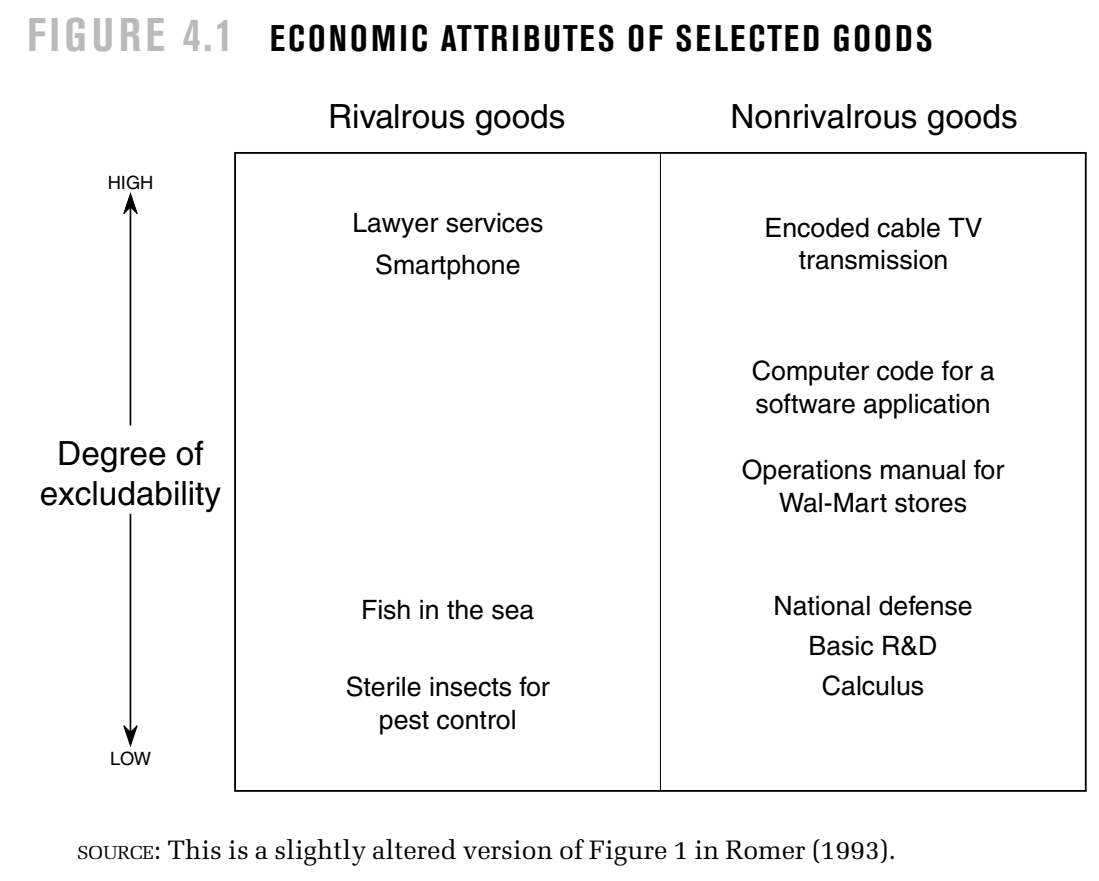
\includegraphics[width=0.7\linewidth]{Imagens/a14i1.png}
\end{figure}

\begin{itemize}
    \item Outra característica das ideias: não-excludência.
    \item Os knowledge spillovers (transbordamentos de conhecimento) 
          implicam que o retorno social das invenções 
          tende a ser maior que o retorno privado.
    \item Resultado:
          \begin{itemize}
            \item Possível subinvestimento em P\&D.
            \item Solução parcial via instituições (leis de patentes etc.).
          \end{itemize}
\end{itemize}


\subsection{\textbf{O Modelo de ``Endogenous Technological Change''}}
Referência: Romer (1990) -- versão Jones (1995).

\subsection{\textbf{Função de produção}}
\[
  Y = K^\alpha \,\bigl(A\,L_Y\bigr)^{1-\alpha},
  \quad (1)
\]
onde:
\begin{itemize}
    \item $K$: capital físico.
    \item $A$: estoque de ideias (tecnologia).
    \item $L_Y$: trabalhadores alocados à produção de bens finais.
\end{itemize}

Esta função apresenta:
\begin{itemize}
    \item Retornos constantes em $K$ e $L_Y$.
    \item Retornos crescentes quando se incorpora a possibilidade de 
          aumento de $A$ (progresso tecnológico).
\end{itemize}


\subsection{\textbf{Componentes do modelo}}
\begin{itemize}
    \item Acumulação de capital:
      \[
        \dot{K} = s_K \,Y - \delta \,K.
      \]
    \item Crescimento da força de trabalho (ou população):
      \[
        \frac{\dot{L}}{L} = n.
      \]
    \item Alocação da força de trabalho:
      \[
        L = L_Y + L_A,
      \]
      onde $L_A$ é o contingente de trabalhadores alocados à pesquisa.
    \item Função de produção de inovações:
      \[
        \dot{A} = \bar{\delta} \,L_A
        \quad \Longrightarrow \quad
        \bar{\delta} = \frac{\dot{A}}{L_A},
        \quad (2)
      \]
      sendo $\bar{\delta}$ a taxa de inovações por pesquisador.
\end{itemize}


\subsection{\textbf{Produtividade da pesquisa e estoque de conhecimento}}
\begin{itemize}
    \item É razoável imaginar que a produtividade em pesquisa, 
          $\bar{\delta}$, dependa de $A$ (estoque de conhecimento), por dois motivos:
          \begin{enumerate}
            \item As ideias geradas no passado aumentam a produtividade dos pesquisadores 
                  no presente (``standing on giants' shoulders''), ou seja, 
                  $\bar{\delta}$ depende positivamente de $A$.
            \item Talvez as primeiras descobertas (``fáceis'') sejam de fato mais simples 
                  do que as descobertas subsequentes (``fishing out effect''), 
                  o que implicaria dependência negativa de $A$.
          \end{enumerate}

    \item Modelo geral:
      \[
        \bar{\delta} = \delta\,A^\phi,
        \quad (3)
      \]
      onde $\delta$ e $\phi$ são constantes:
      \begin{itemize}
        \item $\phi > 0$ reflete o primeiro caso (aumentos de conhecimento facilitam novas descobertas).
        \item $\phi < 0$ reflete o segundo caso (descobertas fáceis primeiro).
        \item $\phi = 0$ significa que $\bar{\delta}$ não depende de $A$.
      \end{itemize}
\end{itemize}


\subsection{\textbf{Papel do número de pesquisadores na produtividade em pesquisa}}
\begin{itemize}
    \item É possível que a produtividade em pesquisa, 
          $\dot{A}/L_A$, dependa também do número de pesquisadores $L_A$.
    \item Exemplo: se há duplicação de esforços de pesquisa 
          (``stepping on others' toes''), 
          o rendimento marginal de novos pesquisadores pode ser decrescente.
    \item Uma formulação comum:
      \[
        \dot{A} = \delta\,L_A^\lambda\,A^\phi, 
        \quad 0 < \lambda < 1,
        \quad (4)
      \]
      levando a
      \[
        \frac{\dot{A}}{L_A}
        = 
        \delta\,L_A^{\,\lambda - 1}\,A^\phi,
        \quad
        \text{decrescente em } L_A \text{ se } \lambda < 1.
      \]
\end{itemize}

\(0 < \lambda < 1\) duplicações de esforços de pesquisa, \textit{"patent races"}


\subsection{\textbf{Discussão segundo Jones (1995)}}
\begin{itemize}
    \item Jones (1995) enfatiza a condição $\phi < 1$. \begin{itemize}
        \item se \(\phi<0\) \textit{"Fishing-out"} effect
        \item se \(\phi>0\) \textit{"Standing on the shoulders of giants"}      
    \end{itemize}
    \item Se $\phi = 1$ (como nos modelos fundadores), a partir de (4) teríamos:
      \[
        \frac{\dot{A}}{A}
        = 
        \delta\,L_A^\lambda.
      \]
      Com $L_A$ constante, essa taxa de inovações seria constante, implicando 
      crescimento constante de $A$ ao longo do tempo. 
    \item Porém, isso é empiricamente incompatível com fatos estilizados:
      \begin{itemize}
        \item O número de cientistas e engenheiros empregados em P\&D 
              cresce ao longo do tempo.
        \item O número de patentes registradas se mantém aproximadamente constante 
              em certos períodos (por exemplo, nos EUA).
      \end{itemize}
    \item Logo, se ao longo do tempo $A$ cresce, então $\dot{A}$ também cresce; 
          mas manter a mesma $L_A$ e obter sempre a mesma taxa $\dot{A}/A$ 
          significaria que cada pesquisador estaria descobrindo 
          cada vez mais invenções — o que não condiz com os dados.
\end{itemize}


\subsection{\textbf{Reescrevendo a equação de inovações}}
Aceitando a especificação de (4), temos:
\[
  \dot{A} = \delta\,A^\phi\,L_A^{\lambda}.
\]
Assim,
\[
  \frac{\dot{A}}{L_A}
  = 
  \delta\,L_A^{\,\overbrace{\lambda - 1}^{<0}}\,A^\phi,
\]
ou combinações semelhantes que resultam em $\bar{\delta}$ decrescente em $L_A$ se $\lambda < 1$.


Dois aspectos importantes da chamada ``economia das ideias'' captados pelo modelo:
\begin{enumerate}
    \item Falácia da composição:
          \begin{itemize}
            \item Um pesquisador (ou empresa) individual enxerga apenas 
                  $\dot{A} = \delta\,L_A$, 
                  como se os retornos da atividade de pesquisa fossem constantes.
            \item Formalmente: 
              \[
                \frac{d\dot{A}}{dL_A}
                = 
                \bar{\delta}
                \quad(\text{constante, para o agente individual}).
              \]
            \item Na verdade, pela (4):
              \[
                \frac{d\dot{A}}{dL_A}
                = 
                \delta\,A^\phi\,\lambda\,L_A^{\lambda - 1},
                \quad
                \text{decrescente em } L_A \text{ se } \lambda<1.
              \]
            \item Essa miopia (desconsiderar o efeito negativo sobre 
                  a produtividade agregada de pesquisa) pode levar 
                  a superinvestimento em P\&D no equilíbrio de mercado, 
                  ou a desalocações ineficientes, dependendo do modelo.
          \end{itemize}

    \item Quando $\phi > 0$, a presença de externalidade positiva 
          (conhecimento atual impulsiona descobertas futuras) 
          pode levar a subinvestimento em P\&D:
          \begin{itemize}
            \item Os inventores se apropriam apenas dos ganhos estáticos 
                  decorrentes de $\Delta A \Rightarrow \Delta Y$.
            \item Mas dinamicamente, $\uparrow A$ hoje facilita novo aumento de $\uparrow A$ 
                  no período seguinte, e assim por diante.
            \item Existe, portanto, externalidade positiva da pesquisa, 
                  gerando possível subinvestimento privado em P\&D.
          \end{itemize}
\end{enumerate}

\newpage
\section{\textbf{Romer 2}}
\subsection{\textbf{Crescimento no modelo de Romer}}

Retomemos a expressão (1) acima:
\[
Y = K^\alpha \cdot (A \cdot L_y)^{1 - \alpha}
\]

Supondo que "capital" é apenas "produto poupado", então no BGP (balanced growth path, trajetória de crescimento equilibrado) é preciso que a relação capital/produto ou produto/capital seja constante ao longo do tempo:

\[
\frac{Y}{K} = K^{\alpha - 1} \cdot A^{1 - \alpha} \cdot L_y^{1 - \alpha}
\]

\[
\Rightarrow \frac{K}{Y} = \left( \frac{K}{A \cdot L_y} \right)^{1 - \alpha} = \left( \frac{K / L_y}{A} \right)^{1 - \alpha}
\]

\[
\Rightarrow \text{se } A \text{ cresce a uma taxa } \frac{\dot{A}}{A} = g_A, \text{ então } \frac{K}{Y} \text{ é constante}
\]

\[
\Leftrightarrow \frac{(K / L_y)}{K / L_y} = g_A \Rightarrow \left( \frac{K / L}{K / L} \right) = g_A \quad \text{(já que no BGP } \frac{L_y}{L} \text{ é constante)}
\]

\[
\left( \frac{L_y}{L} \text{ constante } \Rightarrow \frac{\dot{L}_y}{L_y} = n \equiv \frac{\dot{L}}{L} \right)
\]

\[
\Rightarrow \frac{\dot{K}}{K} = g_A + n, \text{ no BGP. E } \frac{\dot{\mathcal{k}}}{\mathcal{k}} = g_K
\]

Agora, por (1) também temos que...

\[
\frac{Y}{L} = K^\alpha \cdot A^{1 - \alpha} \cdot \frac{L_y^{1 - \alpha}}{L}
\]

\[
= K^\alpha \cdot A^{1 - \alpha} \cdot \left( \frac{\overbrace{\beta}^\text{Fração de Trabaladores} \cdot L}{L} \right)^{1 - \alpha}
= K^\alpha \cdot A^{1 - \alpha} \cdot \beta^{1 - \alpha} \cdot L^{1 - \alpha}
\]

\[
= A \cdot \left( \frac{K / L}{A} \right)^\alpha \cdot \beta^{1 - \alpha}
= A \cdot \left( \frac{K}{A L} \right)^\alpha \cdot \beta^{1 - \alpha}
\]

Como já vimos que no BGP \( g_K = g_A \), temos que \( \frac{\mathcal{k}}{A} \) é constante, e portanto \( \frac{Y}{L} \) só cresce por causa do primeiro termo, \( A \). Logo,

\[
g_y \equiv \frac{\dot{y}}{y} = \frac{\dot{(Y/L)}}{Y/L} = g_A
\]

\textbf{Conclusão:} nesse modelo, \( g_\mathcal{k} = g_y = g_A \). Resta então determinar \( g_A \). Para isso, vamos dividir ambos os lados da equação (4) acima por \( A \), obtendo:

\[
\frac{\dot{A}}{A} = \delta \cdot L_A^\lambda \cdot A^{\phi - 1}
= \frac{\delta \cdot L_A^\lambda}{A^{1 - \phi}} \tag{5}
\]

Ao longo do BGP, \( g_A \) é constante. Formalmente, a partir de (5):

\[
d g_A = 0 \Rightarrow d(\delta \cdot L_A^\lambda \cdot A^{\phi - 1}) = 0
\]

\[
\Rightarrow d\delta \cdot (L_A^\lambda \cdot A^{\phi - 1}) + \delta \cdot d(L_A^\lambda \cdot A^{\phi - 1}) = 0
\]

\[
\Rightarrow d(L_A^\lambda \cdot A^{\phi - 1}) = 0 \Rightarrow
\]

\[
\Rightarrow \lambda \cdot L_A^{\lambda - 1} \cdot \dot{L}_A \cdot A^{\phi - 1}
+ L_A^\lambda \cdot (\phi - 1) \cdot A^{\phi - 2} \cdot \dot{A} = 0
\]

\[
\Rightarrow \lambda \cdot \frac{\dot{L}_A}{L_A} \cdot L_A^\lambda \cdot A^{\phi - 1}
+ L_A^\lambda \cdot (\phi - 1) \cdot A^{\phi - 1} \cdot \frac{\dot{A}}{A} = 0
\]

\[
\Rightarrow \lambda \cdot \frac{\dot{L}_A}{L_A} + (\phi - 1) \cdot \underbrace{\frac{\dot{A}}{A}}_{g_A} = 0 \tag{6}
\]

Se \( \frac{L_A}{L} \) é constante, então \( \frac{\dot{L}_A}{L_A} = \frac{\dot{L}}{L} = n \).

Substituindo isso em (6) e rearranjando, obtemos:

\[
g_A = \frac{\lambda \cdot n}{1 - \phi} \tag{7}
\]

\(\Rightarrow\) essa expressão nos fornece muitas mensagens interessantes:

Em 1\textsuperscript{o} lugar, imagine que \( \lambda = 1 \) (não há duplicação dos esforços de pesquisa) e \( \phi = 0 \) (o conhecimento passado não influencia as descobertas presentes). Nesse caso, a expressão (4) nos diz que:

\[
\dot{A} = \delta \cdot L_A^\lambda \cdot A^\phi = \delta \cdot L_A \Rightarrow \frac{\dot{A}}{L_A} = \delta
\]

\(\Rightarrow\) produtividade constante em pesquisa: cada pesquisador produz \( \delta \) inovações por unidade de tempo. Com \( L_A \) constante, teríamos \( \dot{A} \) constante e, portanto, \( \frac{\dot{A}}{A} \) convergiria para zero conforme \( A \) crescesse.

Pelo contrário, um crescimento \( g_A \) constante só é obtido se \( \dot{A} \) aumentar junto com \( A \), o que requer crescimento de \( L_A \). Formalmente:

\[
\frac{\dot{A}}{A} \equiv g_A = \frac{\delta \cdot L_A}{A} \Rightarrow \text{é preciso que } L_A \text{ cresça a uma taxa igual à taxa de crescimento de } A
\]

\[
\Rightarrow \frac{\dot{L}_A}{L_A} = n = g_A
\]

que é o resultado obtido por (7) acima com \( \lambda = 1 \) e \( \phi = 0 \).

\begin{center}
\fbox{
    \parbox{0.85\linewidth}{
        \textbf{Contraste com o modelo de Solow:} aqui, quanto maior \( n \), maior o crescimento, e portanto o nível da renda per capita também cresce.
    }
}
\end{center}

\textbf{Em 2\textsuperscript{o} lugar} (tal como fez Romer originalmente), suponha que \( \lambda = 1 \) e \( \phi = 1 \), i.e.,

\[
\dot{A} = \delta \cdot L_A \cdot A \Rightarrow \frac{\dot{A}}{A} = \delta \cdot L_A
\]

\(\Rightarrow\) um número constante de pesquisadores (\( L_A \)) é capaz de sustentar o crescimento econômico.

Por (3), teríamos \( \overbrace{\bar{\delta}}^{\frac{\dot{A}}{L_A}} = \delta \cdot A \Rightarrow \) a produtividade em pesquisa é proporcional ao estoque de conhecimento. 

Com \( A \) crescendo, um mesmo número de pesquisadores produziria cada vez mais descobertas. 

\(\Rightarrow\) Já vimos que isso é incompatível com um fato estilizado (pg. 11). Mas também podemos colocar essa incompatibilidade de outra maneira significativa:

\[
\frac{d g_A}{d L_A} = \delta > 0
\]

\(\Rightarrow\) i.e., se \( L_A \) cresce, por exemplo, se há crescimento populacional, a taxa de crescimento \( g_A = g_y \) deveria crescer!

Mas \( g_y \) tem sido aproximadamente \( \simeq 1{,}8\% \) a.a. nos EUA ao longo dos últimos cem anos, apesar de \( n_{USA} \ne 0 \).

\textbf{Conclusões:} se aceitarmos como valores razoáveis para os parâmetros \( \lambda \in (0,1) \) e \( \phi \in (0,1) \), a expressão (7) nos leva a uma conclusão parecida com a do modelo neoclássico de crescimento (Solow): 

\[
g_A \text{ não depende de } s_K \text{ (taxa de poupança )} \Rightarrow \]
\[
\text{ acumulação de capital) nem de } \frac{L_A}{L} 
\text{ (proporção dos trabalhadores ocupados em pesquisa),}
\]

variáveis que poderiam ser afetadas por políticas como poupança compulsória ou subsídios para P\&D. Esse é o “grande resultado” de Jones (1995), que o distingue de Romer, Aghion \& Howitt, Grossman \& Helpman, etc.


\textbf{Um exercício de estática comparativa:} efeitos de um aumento permanente em \( \frac{L_A}{L} \)

Para simplificar, voltemos ao caso \( \lambda = 1 \) e \( \phi = 0 \)

\[
\Rightarrow \text{ por (5) acima } \Rightarrow \frac{\dot{A}}{A} = \delta \cdot \frac{L_A}{A} \tag{8}
\quad \text{com } \frac{\dot{A}}{A} \equiv g_A
\]

Com \( L_A = \underbrace{s_R}_\text{(share in research)} \cdot L \), a equação (8) fica:

\[
g_A = \delta \cdot s_R \cdot \frac{L}{A} \tag{9}
\]

Imagine que a economia estava em \textit{steady-state}, com \( g_A = n \) (o que segue de (7), com \( \lambda = 1 \) e \( \phi = 0 \)).

Agora, suponha que \( s_R \) dá um salto discreto, instantâneo, para \( s_R' > s_R \). Isso leva a \( \uparrow \frac{L_A}{A} \), o que, por (8),

\[
\Rightarrow \uparrow g_A \text{ para } g_A > n
\]

Isso, por sua vez, faz com que \( A \) cresça mais rápido do que \( L_A \), levando a 

\[
\downarrow \frac{L_A}{A} \text{ ao longo do tempo.}
\]

Novamente, por (8), isso faz com que \( g_A \) caia ao longo do tempo, até que se atinja novamente \( g_A = n \).


\begin{figure}[H]
    \centering
    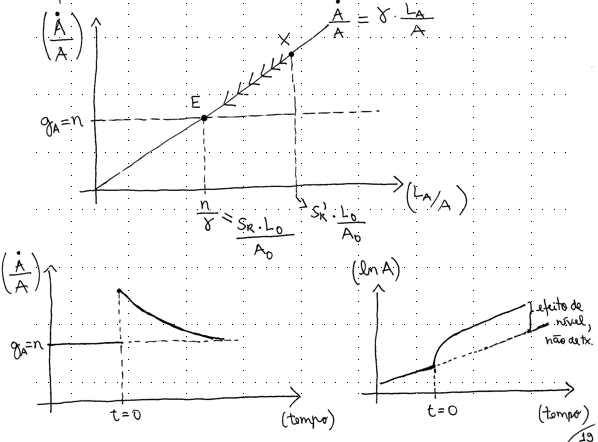
\includegraphics[width=0.7\linewidth]{Imagens/a15i1.png}
\end{figure}

\newpage
\section{\textbf{Romer 3}}

Até agora, nossa análise do papel da inovação (geração de ideias, $\uparrow A$) no processo de crescimento foi puramente ``tecnológica''.

Vamos agora introduzir conteúdo econômico, acrescentando estrutura ao modelo, para:

\begin{itemize}
  \item mostrar como uma economia de mercado pode
  \item gerar crescimento endógeno.
\end{itemize}

\subsection{\textbf{Economia a 3 setores}}

\begin{itemize}
  \item \textbf{Setor de pesquisa (P\&D)}(tudo começa aqui):
  \[
  (L_A, A) \rightarrow \dot{A} \quad \text{(novas ideias, novos designs de bens de capital)}
  \]
  Vende \textbf{patente} para:
  
  \item \textbf{Setor de bens intermediários (bens de capital)}:
  \begin{quote}
    ``aluga'' 1 unidade do bem final $\rightarrow$ 1 unidade de bem de capital \hfill (monopólio). Chegaremos que o custo marginal de produzir uma máquina será a própria taxa de juros.
  \end{quote}
  Vende para:
  
  \item \textbf{Setor de bens finais}:
  \[
  (L_Y, \text{bens de capital}) \rightarrow Y \hfill \text{(concorrência perfeita)}
  \]. Quanto o produtor vai querer colocar de preço no seu produto final.
\end{itemize}

\subsection{\textbf{O setor de bem final}}

Função de produção microeconômica:

\begin{equation}
Y = L_Y^{1 - \alpha} \cdot \sum_{j=1}^{A} x_j^{\alpha}, \quad 0 < \alpha < 1 \tag{10}
\end{equation}

Onde:
\begin{itemize}
  \item $L_Y$ = trabalho alocado para produção de bem final
  \item $A$ = número de bens intermediários disponíveis (bens de capital). Variedade, quantos tipo de máquina que existem. \(\sum_{j=1}^{A}x_j=K\). Alguns economistas usavam o term "\textit{love of variety}"(Dixit \& Stiglitz 1977).\begin{itemize}
      \item \(\alpha=1/2\) , \(L_y=1\) e \(K=12\)
      \item 
      \[
      max \ Y = \sum_{j=1}^{A} x_{j}^{\alpha=1/2}
      \]
      \[
      s.a \ \sum_{j=1}^{A} x_{j} = 12
      \]
      \[
      Se \ \ A = 1 \ , \ x_1^*=12  \ ,\ Y=\sqrt{12}=3,46
      \]
      \[
      Se \ \ A = 2 \ , \ x_1^*= 6 \ , \ x_2^*=6   \ ,\ Y=2\sqrt{6}=4,90
      \]
      \[
      Se \ \ A = 3 \ , \ x_1^*= 4 \ , \ x_2^*=4 \ , \ x_3^*= 4  \ ,\ Y=3\sqrt{4}=6
      \]
      A diversificação aumenta o produto. \(Y\) é cresecente em \(A\), mesmo com o \(K=\bar{K}\)
  \end{itemize}
  \item $x_j$ = quantidade de bem intermediário $j$ utilizada
\end{itemize}

Num dado instante de tempo, com $A$ constante, podemos escrever (10) como:

\begin{equation}
Y = L_Y^{1 - \alpha} \cdot x_1^{\alpha} + L_Y^{1 - \alpha} \cdot x_2^{\alpha} + \cdots + L_Y^{1 - \alpha} \cdot x_A^{\alpha} \tag{10'}
\end{equation}

\begin{itemize}
  \item[$\Rightarrow$] Claramente apresenta \textbf{retornos constantes de escala}: dobrando $L_Y$ e cada $x_j$, dobra-se $Y$.
  \item[$\Rightarrow$] \textbf{Concorrência perfeita}: as empresas desse setor vão tomar $p_Y$ (preço do bem final), $w$ (salário), e $p_j$ (preço do bem de capital $j$) como dados.
\end{itemize}

\subsection{\textbf{Maximização de lucro no setor de bens finais}}

Adotando a normalização $p_Y = 1$ (o bem final é o ``numeraire''), e supondo que há um contínuo $[0, A]$ de bens de capital, o que permite escrever (10) como:

\begin{equation}
Y = L_Y^{1 - \alpha} \cdot \int_0^A x_j^{\alpha} \, dj \tag{10''}
\end{equation}

Coloca-se para o produtor de bem final o seguinte problema de maximização de lucro:

\begin{equation}
\max_{L_Y, x_j} \quad \underbrace{\underbrace{1}_{p_Y} \cdot L_Y^{1 - \alpha} \cdot \int_0^A x_j^{\alpha} \, dj}_{Receita} \ \underbrace{ \  - \omega \cdot L_Y - \int_0^A p_j \cdot x_j \, dj}_{Gasto} \tag{11}
\end{equation}

\vspace{0.2cm}
\noindent\textbf{Condições de 1ª ordem(Demanda por trabalho e Demanda por maquina):}

\begin{equation}
\frac{\partial \text{lucro}}{\partial L_Y} = 0 
\Rightarrow \underbrace{(1 - \alpha) \cdot \frac{Y}{L_Y}}_\text{valor do produto marginal do trabalho} = \omega \tag{12}
\end{equation}

\begin{equation}
\frac{\partial \text{lucro}}{\partial x_j} = 0 
\Rightarrow \underbrace{\alpha \cdot L_Y^{1 - \alpha} \cdot x_j^{\alpha - 1}}_\text{valor do produto marginal do bem de capital $j$} = p_j \tag{13}
\end{equation}

\begin{equation}
    x_j=p_j^{-\frac{1}{1-\alpha}}\alpha^{\frac{1}{1-\alpha}}L_y \tag{13'}
\end{equation}


\subsection{\textbf{O setor de bens intermediários (de capital)}}

Uma vez que o projeto do bem intermediário $j$ foi adquirido por uma empresa deste setor, ela se torna (via proteção patentária) a monopolista nessa variedade de $j$. Isso representa:

\begin{itemize}
  \item um custo fixo (inicial) para a empresa.
\end{itemize}

Depois, a firma, para gerar unidades \textit{físicas} do bem de capital $j$, usa uma tecnologia muito simples: cada unidade de $j$ é produzida com uma unidade de ``capital bruto'' (produto final poupado, o $K$ de antes).

Para utilizar 1 unidade de $K$, o produtor de bem intermediário precisa pagar o ``custo de uso'' do capital, que é igual a $r$ (equivale à taxa de juros).

Ou seja:

\[
1 \text{ unidade de bem intermediário} \quad \Rightarrow \quad \text{custo} = r 
\]

Como disse Keynes(de acordo com o professor) : "Juros é o custo de uso do capital"

Se essa tecnologia de produção e esse custo $r$ valem para todo $j$, e se os diversos bens intermediários entram \textbf{simetricamente} na função de produção (10''), então...

\subsection{\textbf{Demanda e precificação no setor intermediário}}

Sabemos que $x_j = x$ e $p_j = p$ para todo $j$ (as maquinas são simétricas, igualmente produtivas e de mesmo custo):

\begin{equation}
x_j = x \quad \text{e} \quad p_j = p \quad , \quad \forall j \tag{14}
\end{equation}

Ou seja, todos os bens intermediários têm o mesmo preço e são demandados na mesma quantidade. 

Com isso, podemos escrever o problema de maximização de lucro do típico produtor de bem intermediário como:

\begin{equation}
\max_{x} \; \pi = p(x) \cdot x - r \cdot x \tag{15}
\end{equation}

Onde $p(x)$ é a demanda inversa dada por (13).

\vspace{0.2cm}
\noindent\textbf{Condição de primeira ordem:}

\[
p'(x) \cdot x + p(x) = r
\Rightarrow \underbrace{\left[ p'(x) \cdot \frac{x}{p(x)} + 1 \right]}_{[\cdot]} = \frac{r}{p(x)}
\Rightarrow p(x) \cdot \left[ \cdot \right] = r
\]

\begin{equation}
p(x) = \frac{1}{\left[ \frac{p'(x) \cdot x}{p(x)} + 1 \right]} \cdot r \tag{16}
\end{equation}

\hfill (este termo dentro da fração é importante)

\noindent O termo $p'(x) \cdot \frac{x}{p(x)}$ é uma elasticidade do tipo:

\[
\frac{p'(x)}{p} \Big/ \frac{x'}{x}, \quad \text{com } x' = \Delta x = 1
\]

\vspace{0.2cm}
\noindent Por (13), temos:

\[
p'(x) = (\alpha - 1) \cdot \alpha \cdot L_Y^{1 - \alpha} \cdot x^{\alpha - 2}
\]

Multiplicando por $\frac{x}{p(x)}$, obtemos:

\[
p'(x) \cdot \frac{x}{p(x)} \equiv \text{elasticidade} = \alpha - 1
\]

\vspace{0.2cm}
Portanto, retomando (16), temos:

\begin{equation}
p(x) = \frac{1}{\text{elasticidade} + 1} \cdot r = \frac{1}{\alpha} \cdot r \tag{17}
\end{equation}

Ou seja, $p(x)$ é uma margem $\frac{1}{\alpha} > 1$ acima do custo marginal $r$. Essa margem...

\subsection{\textbf{Elasticidade de substituição e retorno à função agregada}}

O markup $\frac{1}{\alpha}$ depende do \textbf{grau de substituibilidade} dos diversos bens intermediários na função de produção do bem final (equação 10'').

Se fosse $\alpha = 1$, a equação (10'') viraria:

\[
Y = L_Y^{1 - \alpha} \cdot \int_0^A x_j dj
\]

e os bens intermediários seriam \textbf{substitutos perfeitos}.

Logo, quanto menor $\alpha$, maior o ``poder de monopólio'' ou ``grau de diferenciação'' de cada bem intermediário.

Além disso, note que a demanda total de ``capital bruto'' por parte dos produtores de bens intermediários deve ser igual ao estoque total de capital da economia:

\begin{align*}
\int_0^A x_j dj = K 
&\Rightarrow \text{(dado que $x_j = x$, $\forall j$)} \\
&\Rightarrow A \cdot x = K \Rightarrow x = \frac{K}{A} \tag{18}
\end{align*}

Substituindo (18) em (10''):

\begin{align*}
Y &= A \cdot L_Y^{1 - \alpha} \cdot x^{\alpha}
= A \cdot L_Y^{1 - \alpha} \cdot \left( \frac{K}{A} \right)^{\alpha} \\
&= L_Y^{1 - \alpha} \cdot K^{\alpha} \cdot A^{1 - \alpha}
= K^{\alpha} \cdot (A \cdot L_Y)^{1 - \alpha} \tag{1'}
\end{align*}

\noindent Que é a boa e velha função de produção agregada da qual partimos em (1)!

\subsection{\textbf{Taxa de juros e remuneração do capital}}

Por fim, já podemos calcular a taxa de juros ($r$) dessa economia, assim como o lucro do monopolista de bens intermediários ($\pi$):

Juntando (13) e (18), temos:

\begin{align*}
P(x) &\equiv P = \alpha \cdot L_Y^{1 - \alpha} \cdot \left( \frac{K}{A} \right)^{\alpha - 1} \\
&= \alpha \cdot L_Y^{1 - \alpha} \cdot A^{1 - \alpha} \cdot K^{\alpha - 1} \\
&= \alpha \cdot \frac{Y}{K} \tag{19} \qquad \text{(por 1')}
\end{align*}

Por outro lado, pela equação (17):

\begin{equation}
P = \frac{1}{\alpha} \cdot r
\end{equation}

Fazendo (17) = (19), temos:

\[
\alpha \cdot \frac{Y}{K} = \frac{1}{\alpha} \cdot r 
\Rightarrow r = \alpha^2 \cdot \frac{Y}{K} \tag{20}
\]

Mas, por (1'), vemos que o produto marginal do capital é:

\[
PMg_K \equiv \frac{\partial Y}{\partial K} = \alpha \cdot \frac{Y}{K}
\]

Ou seja, (20) nos diz que no modelo de Romer (1990), o capital recebe como remuneração \textbf{menos que} $PMg_K$ (o capital(K) é explorado, aquele que poupa é explorado).

\subsection{\textbf{Interpretação: concorrência imperfeita e lucro}}

Qual a importância disso?

Bem, com $A$ dado num certo instante (ponto no tempo), a equação (1') exibe \textbf{retornos constantes} em $L_Y$ e $K$. Ou seja, $Y$ é uma função homogênea de grau 1 e vale o \textbf{Teorema de Euler}:

\[
\frac{\partial Y}{\partial L_Y} \cdot L_Y + \frac{\partial Y}{\partial K} \cdot K = Y
\]

\[
rK+wL_Y<Y
\]
\[
rK+w(\underbrace{L_Y+L_A}_L)=Y
\]

Com $\omega = PMg_{L_Y}$, se $r$ fosse igual a $PMg_K$, então não sobraria nada para remunerar os trabalhadores alocados na atividade de pesquisa 
(lembre-se: $L_Y + L_A = L$).

Como em \textbf{concorrência perfeita} todos os fatores devem ser remunerados pela sua produtividade marginal, vemos que o modelo deve \textbf{necessariamente incorporar concorrência imperfeita}...


O lucro ($\pi$) do produtor de bens intermediários é simples de calcular:

\begin{align*}
\pi &= [P - r] \cdot x = \text{por (17)} = \left( \frac{1}{\alpha} - 1 \right) \cdot r \cdot x \\
    &= \text{por (20) e (18)} = \frac{1 - \alpha}{\alpha} \cdot \alpha^2 \cdot \frac{Y}{K} \cdot \frac{K}{A} \\
    &= \alpha \cdot (1 - \alpha) \cdot \frac{Y}{A} \tag{21}
\end{align*}

\textbf{Romer}: Lucro perpétuo, pois as máquinas não se tornam obsoletas.

\[
g_\pi=g_Y-g_A = (g_y+n)-g_A\underbrace{=}_\text{no Steady Statte}\underbrace{g_A}_{\uparrow y}+\underbrace{n}_\text{cresc. pop \(\rightarrow\) Expansão do mercado}-\underbrace{g_A}_{\uparrow Variaedade \rightarrow \downarrow Mkt Share}=n>0
\]

\newpage
\section{\textbf{Romer 4}}
\subsection{\textbf{O setor de pesquisa}}


Já vimos que a geração de novas ideias é descrita por
\[
\dot{A} = \gamma \cdot L_A^\lambda \cdot A^\phi \tag{4, acima}
\]

Um inventor (trabalhador dedicado à pesquisa) recebe do governo uma patente protegendo sua invenção, que no modelo consiste no segredo de fabricação de um novo bem intermediário, a partir do capital bruto.

Essa patente é vendida a um preço $P_A$ para uma empresa do setor de bens intermediários.

Em equilíbrio, se a patente é valorizada "de acordo c/ os fundamentos", então ela vale

\[
P_A = \text{valor presente descontado do fluxo de lucros } \pi \text{ do monopolista do setor de bens intermediários}.
\] 

Livre entrada no setor de máquinas(leilão pela patente).

\[
VPD(\{\pi_t\}^\infty_{t=1})=\left(\pi_0+\frac{\pi_1}{(1+r)^1}+\frac{\pi_2}{(1+r)^2}+\cdots++\frac{\pi_t}{(1+r)^t}\right)-\pi_0
\]
\[
VPD(\{\pi_t\}^\infty_{t=1})=\left(\pi_0+\frac{\pi_0(1+n)^1}{(1+r)^1}+\frac{\pi_0(1+n)^2}{(1+r)^2}+\cdots +\frac{\pi_0(1+n)^t}{(1+r)^t}        \right)-\pi_0
\]
\[
VPD(\{\pi_t\}^\infty_{t=1})=\pi_0\sum_{i=0}^\infty\left(\frac{1+n}{1+r} \right)^i-\pi_0
\]
\[
VPD(\{\pi_t\}^\infty_{t=1})=\pi_0\frac{1}{1-\frac{1+n}{1+r}}-\pi_0
\]
\[
VPD(\{\pi_t\}^\infty_{t=1})=\pi_0\frac{1}{\frac{r-n}{1+r}}-\pi_0
\]
\[
VPD(\{\pi_t\}^\infty_{t=1})=\pi_0\frac{1+r}{r-n}-\pi_0
\]
\[
VPD(\{\pi_t\}^\infty_{t=1})=\frac{\pi_0(1+n)}{r-n}
\]
\[
VPD(\{\pi_t\}^\infty_{t=1})=\frac{\pi_1}{r-n} \equiv\frac{\pi}{r-n}=P_A
\]
\[
P_A>0\Leftrightarrow \underbrace{r>n}_\text{eficiência dinâmica}\]

\textbf{Uma condição de não-arbitragem descreve o movimento de $P_A$ ao longo do tempo:}

\[
r \cdot P_A = \pi + \dot{P}_A \tag{22}
\]

\begin{center}
\text{rendimento de 1 período de uma aplicação financeira (ou ativo capital $K$) valendo $P_A$} \\
\text{rendimento de 1 período da patente: aufero lucro e depois vendo a patente}
\end{center}

\[
\Rightarrow r = \frac{\pi}{P_A} + \frac{\dot{P}_A}{P_A} \tag{23}
\]

Em equilíbrio de longo prazo (BGP), $r$ deve ser constante, refletindo, digamos, a ``taxa de preferência intertemporal''. Bem,

\[
r \text{ cte.} \Rightarrow \frac{\pi}{P_A} \text{ cte.} \Rightarrow P_A \text{ cresce à mesma taxa que } \pi
\]

Agora, por (21), vimos que $\pi$ era proporcional a $\frac{Y}{A}$. No BGP, temos que
\[
\frac{\dot{Y}}{Y} = n + g_A \quad \text{e} \quad \frac{\dot{A}}{A} = g_A \Rightarrow \frac{Y}{A} \text{ cresce à taxa } n \Rightarrow \pi \text{ cresce à taxa } n
\]

\[
\Rightarrow \frac{\dot{P}_A}{P_A} = n
\]

Logo, no BGP, e por (23), deve valer

\[
P_A = \frac{\pi}{r - n} \tag{24}
\]

\subsection{\textbf{Solução do modelo}}

No modelo de Romer (1990), versão Jones, já vimos que o capital precisa ser sub-remunerado ($r < PMg_K$) a fim de que os trabalhadores alocados em pesquisa ($L_A$) recebam alguma fração de $Y$ (produto final). A estrutura do modelo nos diz como isso acontece:

\[
p > r \quad \Rightarrow \quad \text{renda na mão do monopolista do setor intermediário}
\]

\[
\text{preço do bem intermediário} \quad \text{CMg do monopolista (RMg do monopolista)}
\]

\[
\pi = (p - r) \cdot x
\]

Mas, por (24), vemos que a renda do monopolista paga exatamente o esforço de pesquisa dos trabalhadores $L_A$.

Jones comenta que esse quadro é característico de ``concorrência monopolística'':
\begin{quote}
"não há lucro econômico; todas as rendas compensam algum insumo de fator."
\end{quote}

Mas, para isso ser verdade, resta ainda impor que a remuneração de $L$ no setor de pesquisa seja igual à remuneração no setor de bens finais. Isso é feito supondo livre mobilidade do trabalho entre esses setores.

Já vimos em (12) que

\[
\omega_Y = (1 - \alpha) \cdot \frac{Y}{L_Y}
\]

\begin{center}
\text{salário no setor de bens finais}
\end{center}

Por outro lado, no setor de pesquisa, vamos supor que os trabalhadores consideram sua produtividade como dada. Em termos de (4  ;  \(\dot{A}=\gamma L_A^\lambda A^\phi\)) acima, é como se $\lambda = 1$ e $\phi = 0$, implicando

\[
\dot{A} = \gamma \cdot L_A \quad \Rightarrow \quad \frac{\partial \dot{A}}{\partial L_A} = \gamma
\]

\begin{center}
\text{produto marginal do trabalho no setor de pesquisa}
\end{center}

Se esse setor for competitivo, então:
\[
\underbrace{\omega_R}_\text{salário no setor de pesquisa (R)} = \underbrace{\gamma \cdot P_A}_\text{valor do produto marginal} \tag{25}
\]

Fazendo (12) = (25), vem
\[
\omega_Y = \omega_R \Rightarrow (1 - \alpha) \cdot \frac{Y}{L_Y} = \gamma \cdot P_A
\Rightarrow
\]

Pelo (24),
\[
(1 - \alpha) \cdot \frac{Y}{L_Y} = \gamma \cdot \frac{\pi}{r - n}
\Rightarrow
\]

Pelo (21),
\[
(1 - \alpha) \cdot \frac{Y}{L_Y} = \frac{\gamma}{r - n} \cdot \alpha (1 - \alpha) \cdot \frac{Y}{A}
\Rightarrow
\]

\[
\frac{1}{L_Y} = \frac{\alpha}{r - n} \cdot \frac{\gamma}{A} \tag{26}
\]

Mas, com $L_A$ sendo "ofertado" por trabalhadores que enxergam $\dot{A} = \gamma \cdot L_A$, e com $\frac{\dot{A}}{A} = g_A$ no BGP, (26) fica:

\[
\frac{1}{L_Y} = \frac{\alpha}{r - n} \cdot \frac{g_A}{L_A}
\Rightarrow
\]

\[
\frac{L_A}{L_Y} = \frac{\alpha \cdot g_A}{r - n}
\Rightarrow
\]

\[
\frac{L_A}{L - L_A} = \frac{\alpha \cdot g_A}{r - n}
\Rightarrow
\]

\[
\frac{L}{L_A} - 1 = \frac{r - n}{\alpha \cdot g_A}
\Rightarrow
\]

\[
\underbrace{\frac{L_A}{L}}_{\equiv s_r} = \frac{1}{1 + \frac{r - n}{\alpha \cdot g_A}} \tag{27}
\]

\[
s_r \equiv \text{fração ou share de trabalhadores em pesquisa}
\]

Por (27), vemos que:

\[
\frac{\partial s_r}{\partial g_A} > 0 \quad \text{,} \quad \frac{\partial s_r}{\partial (r - n)} < 0 \quad \text{,} \quad \frac{\partial s_r}{\partial n} > 0 \quad \text{e} \quad \frac{\partial s_r}{\partial r} < 0 
\]

\[
\underbrace{s_R^*}_\text{steady-statte}=\frac{1}{1+\frac{r-n}{\alpha \underbrace{n}_\text{válido somente no Steady Satte}}} \tag{27'}
\]

\subsection{\textbf{Eficiência da alocação de trabalho em pesquisa}}

Chamemos a alocação de trabalhadores para pesquisa resultante de uma economia de mercado de $s_r^{\text{MKT}}$, dada pela expressão (27) acima. Será essa alocação socialmente ótima ($= s_r^{\text{ótima}}$)?

Se os trabalhadores (ou firmas que contratam os trabalhadores) no setor de P\&D tomassem a verdadeira expressão (4),

\[
\dot{A} = \gamma \cdot L_A^\lambda \cdot A^\phi \Rightarrow
\frac{\partial \dot{A}}{\partial L_A} = \gamma \cdot \lambda \cdot L_A^{\lambda - 1} \cdot A^\phi = \omega_R \tag{28}
\]

Fazendo (28) = (12), i.e., $\omega_R = \omega_Y$, usando (24) e (21), mais o fato de que no BGP deve ser agora $g_A = \frac{\dot{A}}{A} = \gamma \cdot L_A^\lambda \cdot A^{\phi - 1}$, chegamos a uma expressão idêntica à (27):

\[
s_r^{\text{ótima}} = \frac{1}{1 + \frac{r - n}{\alpha \cdot g_A}} \tag{29}
\]

Porém, o $g_A$ daqui não é o mesmo de (27). Lá, $g_A^{\text{MKT}} = \gamma \cdot \frac{L_A}{A}$, enquanto aqui:

\[
g_A^{\star} = \gamma \cdot L_A^\lambda \cdot A^{\phi - 1}
\Rightarrow
g_A^{\text{MKT}} = (\gamma \cdot \frac{L_A}{A}) = g_A^{\star} \cdot L_A^{1 - \lambda} \cdot A^{-\phi}
\Rightarrow
\]

\[
g_A^{\text{MKT}} = g_A^{\star} \cdot L_A^{1 - \lambda} \cdot A^{-\phi} \tag{30}
\]

Ora, como (29) é idêntica a (27), já sabemos que
\[
\frac{ds_r^{\text{MKT}}}{dg_A} = \frac{ds_r^{\text{ótima}}}{dg_A} > 0
\]

Basta então usar (30) para comparar $g_A^{\text{MKT}}$ com $g_A^{\star}$:

\begin{itemize}
    \item $0 < \lambda < 1 \Rightarrow g_A^{\text{MKT}} > g_A^{\star} \Rightarrow s_r^{\text{MKT}} > s_r^{\text{ótima}}$ \\
    (caso de duplicação dos esforços de pesquisa ou “congestionamento”)

    \item $\phi > 0$ (“standing on giants’ shoulders”) \\
    $\Rightarrow g_A^{\text{MKT}} < g_A^{\star} \Rightarrow s_r^{\text{MKT}} < s_r^{\text{ótima}}$

    \item $\phi < 0$ (“fishing-out effect”) \\
    $\Rightarrow g_A^{\text{MKT}} > g_A^{\star} \Rightarrow s_r^{\text{MKT}} > s_r^{\text{ótima}}$
\end{itemize}

Essas duas externalidades (associadas a $\lambda$ e a $\phi$) parecem sugerir o seguinte:

\begin{itemize}
    \item \textbf{Pesquisa aplicada} $\leftrightarrow$ "patent races" $\Rightarrow \lambda$ baixo $\Rightarrow$ excesso de investimento em pesquisa pelo mercado.
    \item \textbf{Pesquisa básica} $\leftrightarrow$ grandes "knowledge spillovers" $\Rightarrow \phi$ alto $\Rightarrow$ falta de investimento pelo mercado $\Rightarrow$ gasto público em universidades e institutos.
\end{itemize}

Além dessas duas externalidades que acabamos de ver, há ainda uma 3ª, melhor compreendida de um ponto de vista mais \textit{agregado} que o do $C_M^K$. Por (24),

\[
P_A = \frac{\pi}{r - n}
\]

de modo que o retorno da pesquisa depende dos lucros de monopólio com um novo bem de capital (intermediário). Mas...


\begin{figure}[H]
    \centering
    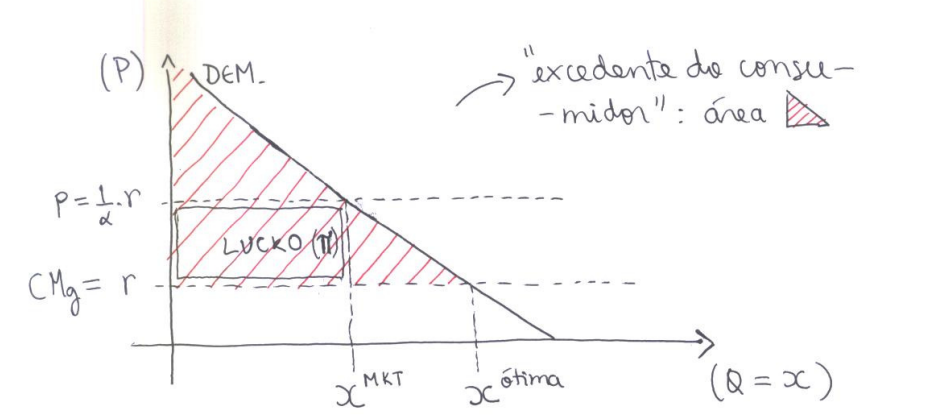
\includegraphics[width=0.7\linewidth]{Imagens/a16i1.png}
\end{figure}


O lucro do monopólio com um novo bem de capital (intermediário) é menor que o excedente do consumidor, e $x^{\text{MKT}} < x^{\text{ótima}}$.

Aqui, a lição é a seguinte: se o monopolista pudesse aumentar seu poder, por exemplo, fazendo discriminação perfeita, então $\pi \Rightarrow$ excedente do consumidor, e aumentaria o bem-estar social.

É por isso que esses modelos de crescimento endógeno são chamados de "Schumpeterianos": \textbf{monopólio é bom!}

\newpage
\section{\textbf{Instituições (Jones, cap.7)}:“Infra-estrutura”(ou Instituições) e desempenho econômico de longo prazo}

\textit{Um paper “clássico”: }Hall and Jones (1998/1999): “Why Do Some Countries Produce So Much More Output per Worker than Others?”

Considere o seguinte modelo de regressão:
\[
y_i = \beta_0 + \beta_1 \cdot s_{ki} + \beta_2 \cdot n_i + \beta_3 \cdot u_i + \beta_4 \cdot s_{Ri} + \beta_5 \cdot \gamma_i + \varepsilon_i
\]

Onde \(\gamma_i\) é o grau de abertura comercial do País.

Aqui temos “fundamentos” vindos dos modelos que estudamos até agora: Solow, Romer, transferência de tecnologia.

Como poderíamos incorporar “instituições”? Mais variáveis do lado direito da equação acima?\begin{itemize}
    \item  \textbf{Não!}
\end{itemize}

Como incorporar \textit{instituições}? $\rightarrow$ como \textit{instrumentos} para as variáveis explicativas do modelo acima!

\begin{itemize}
    \item $s_K \leftrightarrow$ direitos de propriedade, desenvolvimento financeiro (poupança $\rightarrow$ investimento), rentabilidade do investimento
    \item $u \leftrightarrow$ retorno da educação ("college premium"), crédito para educação, natureza da ocupação/atividade econômica (produção vs. \textit{rent seeking})
    \item $s_R \leftrightarrow$ IPRs, leis de patentes
    \item $\gamma \leftrightarrow$ IPRs internacionais, TRIPs, abertura da economia
\end{itemize}


\subsection{\textbf{O Problema do Investimento Empresarial}}
Considere uma empresa multinacional que pretende instalar uma filial num certo país. Para tomar sua decisão, ela vai comparar:
\[
\underbrace{\pi}_\text{VPDdo Fluxo de Lucros}= \underbrace{F}_\text{Custo Fixo de Instalação}
\]

$F \leftrightarrow$ custos burocráticos (licenças, alvarás de funcionamento, etc.), impostos, corrupção, insegurança e violência

\textbf{Obs.:} a existência de barreiras burocráticas (“red taping”) propicia a corrupção

Instituições favoráveis ou desfavoráveis a um “bom ambiente de negócios”? $\rightarrow$ \\
\texttt{http://portugues.doingbusiness.org/rankings}

$\pi \leftrightarrow$ tamanho do mercado, atividades \textit{rent seeking} e estabilidade política e econômica

\textbf{Tamanho do mercado:} não apenas nacional, mas também potencial exportador, dependendo da abertura da economia

\textbf{Atividades \textit{rent seeking}:} gastos correntes com advogados, lobistas, propinas, etc.

\textbf{Estabilidade:} mudanças de regras, revoluções, expropriações $\rightarrow \uparrow$ incerteza


\subsection{\textbf{A decisão de investir em educação e qualificação}}

Investimento em \textit{capital humano} (produtividade, crescimento, etc.) \quad X \quad investimento em \textit{capital político} (disputa pelo share distributivo de cada indivíduo ou grupo)

David Hume (\textit{“Of the Rise and Progress of the Arts and Sciences”}): diferenças de temperamento e habilidades sob uma \textit{monarquia absoluta} (lisonja, persuasão, etc.) e sob uma monarquia constitucional ou \textit{democracia} (pragmatismo, industriosidade, etc.)

Esses diferentes investimentos/habilidades não são facilmente conversíveis uns nos outros

\subsection{\textbf{Evidências Empíricas}}

Um país que atrai investimentos nas formas de capital para negócios, transferência de tecnologia e qualificação da mão-de-obra será aquele no qual:

\begin{enumerate}
    \item Instituições são estáveis; instituições favorecem a produção e não o desvio $\rightarrow$ medida ``PPAD'' (obtida a partir da consultoria \url{http://www.prsgroup.com/})

    \item Economia é aberta ao comércio internacional e à concorrência no mercado mundial $\rightarrow$ medida ``abertura'' (percentual de anos em que a economia foi considerada ``aberta'' pela classificação do Banco Mundial, a partir de 1950)
\end{enumerate}


\(a\cdot PPAD + Abertura(1-a)=Infraestrutura \ \ Social\),usada na edição antiga do Jones.


\textbf{World Bank Governance Indicators Project (2010 $\rightarrow$):}

\begin{itemize}
    \item accountability of politicians
    \item political stability
    \item government effectiveness
    \item regulatory quality
    \item extent of the rule of law
    \item control of corruption
\end{itemize}

Uma média simples desses 6 itens é a “\textit{social infrastructure}” da edição atual (Jones \& Vollrath).


\subsubsection{\textbf{Investimento e infraestrutura social}}
\begin{figure}[H]
    \centering
    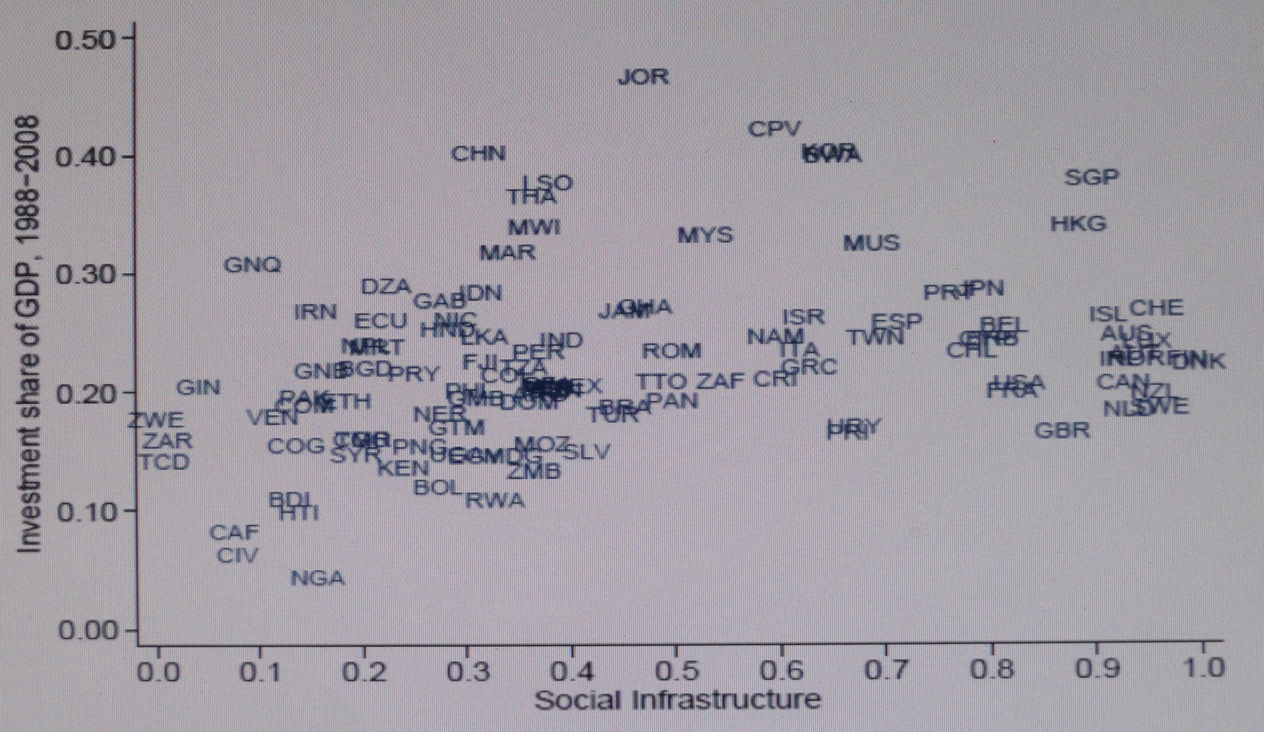
\includegraphics[width=0.7\linewidth]{Imagens/a16i2.png}
\end{figure}

\subsubsection{\textbf{Educação e infraestrutura social}}

\begin{figure}[H]
    \centering
    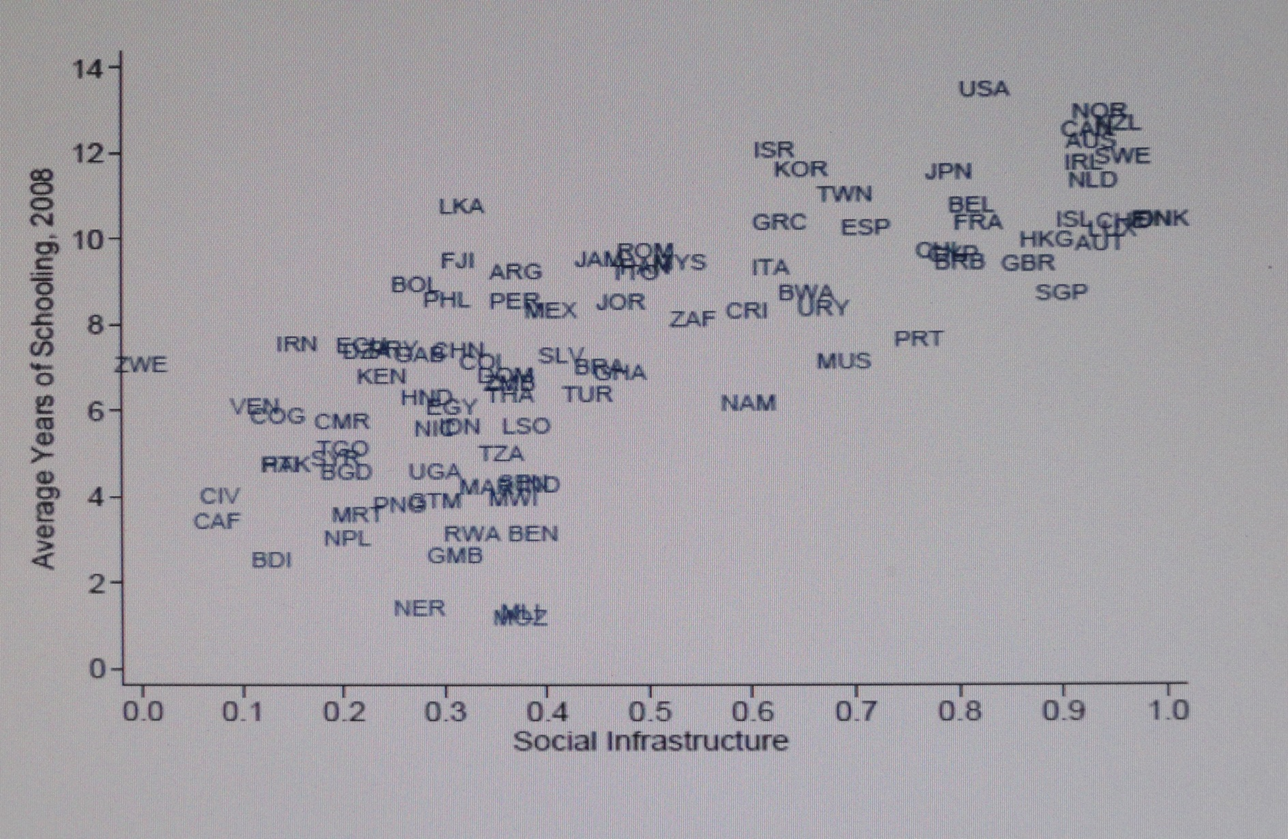
\includegraphics[width=0.7\linewidth]{Imagens/a16i3.png}
\end{figure}

\subsubsection{\textbf{PTF e infraestrutura social}}

\begin{figure}[H]
    \centering
    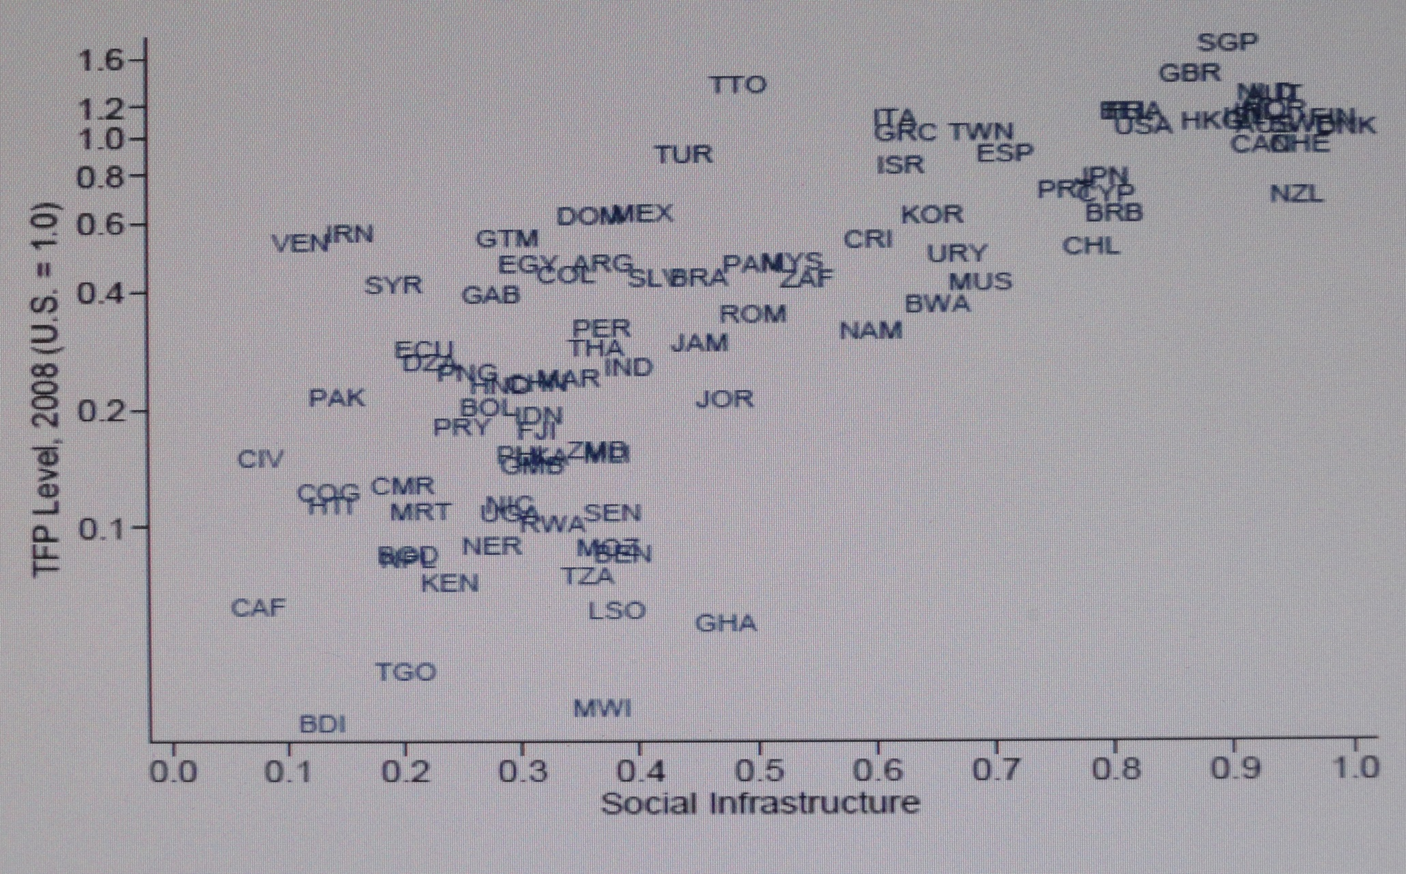
\includegraphics[width=0.7\linewidth]{Imagens/a16i4.png}
\end{figure}

\subsection{\textbf{MISALLOCATION AND PRODUCTIVITY}}
Em países cuja produtividade média na indústria é muito menor do que a dos EUA (como India, Bangladesh, etc.), as firmas dentre as 10\% mais produtivas apresentam produtividade semelhante às top americanas.

O problema é que há muitas firmas de baixíssima produtividade empregando considerável porção do capital e do trabalho ! \(\leftrightarrow\) presença de estatais, setores protegidos, legislação impedindo livre-mobilidade do capital e trabalho entre firmas, setores e regiões da economia.

Evidência de alocação correta: Nos EUA, observamos uma alta correlação positiva entre tamanho e produtividade das firmas.

\subsection{\textbf{Abordagens para a reforma}}
\textit{laundry list} – todas as instituições ao mesmo tempo (Washington Consensus, CGD) \(X\) \textit{growth diagnostics} − identificar distorções mais graves (D. Rodrik)

\subsubsection{\textbf{Críticas}}
\textbf{Laundry list}: falta de capital político, efeitos de equilíbrio geral (2nd best)

\textbf{Growth diagnostics:} restrito a políticas de curto e médio prazo (tarifas, subsídios, crédito, etc.); não chega a haver reforma das instituições

\begin{figure}[H]
    \centering
    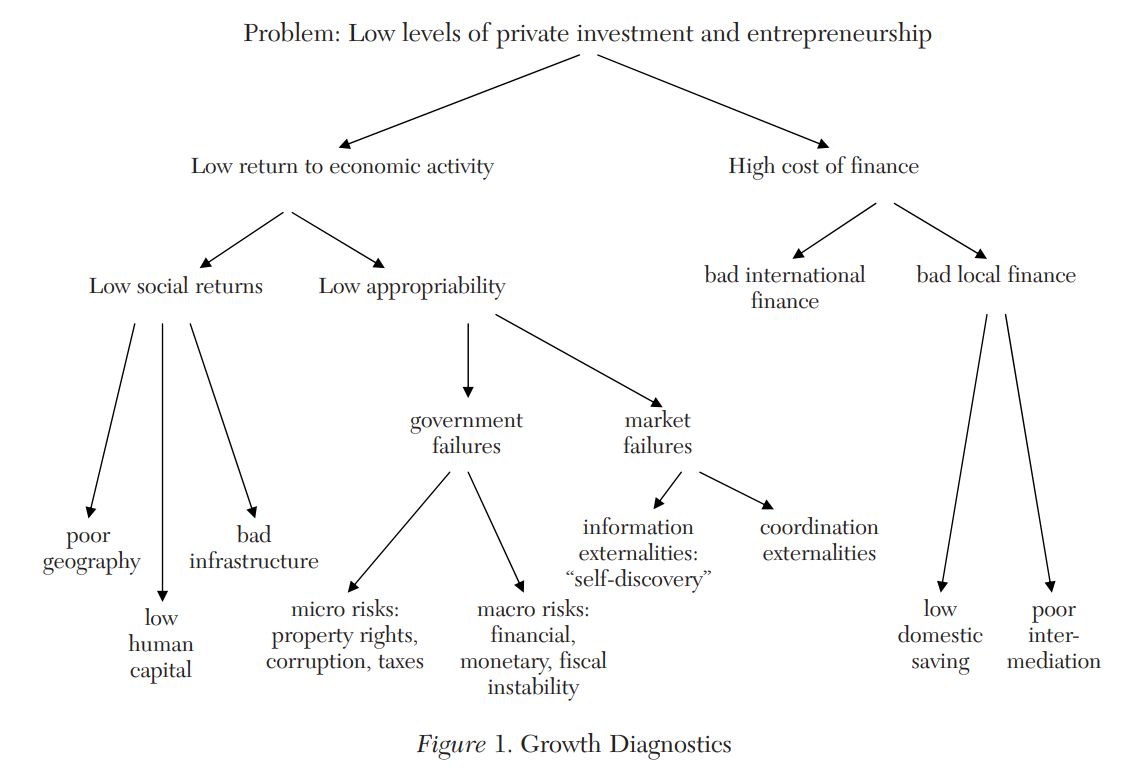
\includegraphics[width=0.7\linewidth]{Imagens/a17i1.png}
\end{figure}

\subsection{\textbf{A escolha da infraestrutura social}}
O grande problema da “economia política” é saber como fazer a transição de um conjunto de instituições ineficientes, que promovem o desvio, para um conjunto virtuoso, que promove a produção e a eficiência \(\leftrightarrow\) problemas de \textit{commitment}, compensação, etc.

D. North, Acemoglu \& Robinson … muito “cabeça”, vamos parar por aqui !!  

\newpage
\section{\textbf{Quality Ladder 1}}

\begin{itemize}
    \item Quality Improvement(\textit{"quality ladder"})\begin{itemize}
        \item Aghion e Howitt(1992, 2005)
        \item Crescimento : aumento da qualidade ou da produtividade de bens já existentes. Bens velhos ficam obsoletos, e seus produtores são lançados para fora do mercado.
        \item \textbf{\textit{"Creative Destruction"}}, Schumpeter
    \end{itemize}
    \item "Variety Expansion"\begin{itemize}
        \item Romer, 1990
        \item Crescimento : aumento do nº de bens existentes
    \end{itemize}
\end{itemize}

\subsection{\textbf{Toy Version}}
O tempo é discreto, indexado por $t = 1,2,\dots$. Em cada ponto do tempo há uma massa $L$ de indivíduos, cada um ofertando inelasticamente $1$ unidade de trabalho qualificado. Indivíduos vivem por um período e maximizam seu consumo no fim desse período.

A cada período há um único bem final, produzido de acordo com
\[
 Y_t \;=\; A_t\,X_t^{\alpha},
 \qquad 0<\alpha<1
 \tag{1}
\]
onde $A_t$ é a qualidade(ou a geração da máquina), no período $t$, do bem intermediário usadona produção do bem final, e $X_t$ é a quantidade empregada desse bem.

Uma unidade de bem intermediário é produzida com uma unidade de trabalho qualificado, de modo que $X_t$ também mede o trabalho usado na produção do bem final.  O trabalho pode, ainda, ser usado em pesquisa, de forma que
\[
 L_t \;=\; L \;=\; \underbrace{X_t}_\text{\(L_y\) do modelo de Romer} + \underbrace{N_t}_\text{\(L_a\) do Romer(Trabalho em Pesquisa)}
 \tag{2}
\]
onde $N_t$ é o trabalho alocado à pesquisa.

%------------------ inovação -------------------------------------
Uma inovação bem-sucedida aumenta a qualidade do insumo intermediário por um fator $\gamma$:
\[
 A \;\longrightarrow\; \gamma\,A, 
 \qquad \gamma>1
 \tag{3}
\]

Se um empresário inovador investir $z$ unidades de trabalho em pesquisa, ele descobre uma nova versão do bem intermediário com probabilidade $\lambda\,z$. O inovador bem-sucedido obtém monopólio na produção dessa nova versão, mas enfrenta \textbf{imitadores} que conseguem produzir a mesma geração do bem usando $\chi>1$ unidades de trabalho por unidade do bem, em vez de $1{:}1$.   Quando $\chi<1/\alpha$, a margem dos imitadores é efetiva (\emph{binding}), de modo que $\chi\,w_t$ é o preço máximo que o inovador pode cobrar sem ser expulso do mercado; $w_t$ é o salário no período $t$.  Assim, o lucro do empresário inovador é
\[
 \pi_t \;=\; (\chi-1)\,w_t\,\chi_t
 \tag{4}
\]

Essa renda de monopólio dura apenas um período; depois disso, assume-se que os imitadores passam a produzir o bem com apenas uma unidade de trabalho.  Considere agora um empresário que investe uma unidade de trabalho em pesquisa no período $t$.  O custo é $w_t$ e o retorno esperado é $\lambda\,\pi_{t+1}$, pois, se bem-sucedido, ele produzirá o novo bem no período seguinte.   Pela expressão \textbf{(4)}, $\pi_t\propto w_t$; além disso, $w_t$ deve igualar o produto marginal do trabalho no bem final.  Inserindo \textbf{(1)}, com $\chi$ constante (o que vale em \emph{steady-state}), temos produto marginal proporcional a $A$, de forma que uma inovação implica
\[
 w_{t+1} = \gamma\,w_t
 \;\;\Longrightarrow\;\;
 \pi_{t+1} = \gamma\,\pi_t .
\]
A condição de \emph{não-arbitragem} (custo = retorno esperado) era
$w_t=\lambda\,\pi_{t+1}$; substituindo o resultado acima,
\[
 w_t \;=\; \lambda\,\gamma\,\pi_t
 \tag{5}
\]

%------------------ sistema fechado -------------------------------
\smallskip
Substituindo \textbf{4} em \textbf{5},
\[
 w_t = \lambda\,\gamma\,(\chi-1)\,w_t\,\chi_t
 \;\;\Longrightarrow\;\;
 1 = \lambda\,\gamma\,(\chi-1)\,\chi_t
 \tag{6}
\]

Em \emph{steady-state}, \textbf{2} implica
\[
 L = X + N \tag{2'}
\]
\[
 X = L - N \tag{2''}
\]

Substituindo \textbf{2''} em \textbf{6},
\[
 1 = \lambda\,\gamma\,(\chi-1)\,\bigl(L-N\bigr)
 \tag{7}
\]

Resolvendo para $N$(número de trabalhadores em P\&D),
\[
 N = L - \frac{1}{\lambda\,\gamma\,(\chi-1)}
 \tag{8}
\]

No Romer tínhamos que a proporção de trabalhadores em P\&D é dado por:
\[
\mathcal{s}_r\equiv\frac{L_A}{L}
\]

Para o Aghion, podemos escrever isso :
\[
\mathcal{s}_r\equiv\frac{N}{L}\rightarrow\frac{N}{L}=1-\frac{1}{L\lambda\gamma(\chi-1)}
\]

\paragraph{\textbf{Sinais}}\;
$\displaystyle
\frac{\partial N}{\partial L}>0,\;
\frac{\partial N}{\partial\lambda}>0,\;
\frac{\partial N}{\partial\gamma}>0,\;
\frac{\partial N}{\partial \chi}>0
$

%------------------ dinâmica de A ---------------------------------
\[
A_t =
\begin{cases}
\gamma\,A_{t-1} & \text{com probabilidade } \lambda\,N, \textbf{Sucesso}\\[4pt]
A_{t-1}         & \text{com probabilidade } 1-\lambda\,N \ \textbf{Fracasso}
\end{cases}
\tag{9}
\]

Podemos chegar em uma formula de "salto de qualidade"
\[
A_t-A_{t-1}\underbrace{=}_\text{se sucesso} \gamma A_{t-1}-A_{t-1}=\underbrace{(\gamma-1)}_{>0}A_{t-1}
\]

A taxa de crescimento esperada da produtividade é
\[
 g_t \;\equiv\;
 \frac{\mathbb{E}(A_t)-A_{t-1}}{A_{t-1}}
 = \underbrace{\lambda\,N}_\text{frequência de inovação}\,\overbrace{(\gamma-1)}^\text{tamanho da inovação}
 \tag{10}
\]

Por \textbf{8} e \textbf{10},
\[
 g_t \;=\;
 \lambda\,
 \Bigl[L - \dfrac{1}{\lambda\,\gamma\,(x-1)}\Bigr]
 (\gamma-1)
 \tag{11}
\]

%------------------ corolários de política ------------------------
\paragraph{\textbf{Corolários de política}}
\begin{align*}
\frac{\partial g_t}{\partial L} &> 0
\;\;\Longrightarrow\;\; \text{investir em educação / capital humano};\\[2pt]
\frac{\partial g_t}{\partial\lambda} &> 0,\;
\frac{\partial g_t}{\partial\gamma} > 0
\;\;\Longrightarrow\;\; \text{investir em pesquisa básica (e aplicada)};\\[2pt]
\frac{\partial g_t}{\partial \chi} &> 0
\;\;\Longrightarrow\;\; \text{elevar o custo de imitação $\;\Rightarrow\;$ garantir I.P.R.s.}
\end{align*}
%-----------------------------------------------------------------

\subsection{\textbf{Demanda por \(x\)}}

\[
\max_x \left( \frac{A \cdot x^\alpha}{\gamma} - P_M \cdot x \right) 
\quad \text{preço do monopolista}
\]

FOC:
\[
\alpha \cdot A \cdot x^{\alpha - 1} = P_M
\Rightarrow
x = \left( \frac{P_M}{\alpha A} \right)^{\frac{1}{\alpha - 1}}
= \left( \frac{A \alpha}{P_M} \right)^{\frac{1}{1 - \alpha}} \quad (\text{pois } \alpha < 1)
\]

\subsection{\textbf{Monopolista}:}

\[
\max_{P_M} \left\{ P_M \cdot x(P_M) - x(P_M) \cdot \omega \right\}
\]

Substituindo \(x(P_M)\):

\[
\max_{P_M} \left\{
P_M \cdot \left( A \alpha \right)^{\frac{1}{1 - \alpha}} \cdot P_M^{\frac{\alpha}{\alpha - 1}}
-
\left( A \alpha \right)^{\frac{1}{1 - \alpha}} \cdot P_M^{\frac{1}{\alpha - 1}} \cdot \omega
\right\}
\]

\[
\Rightarrow \max_{P_M} \left\{
P_M^{\frac{\alpha}{\alpha - 1}} - \omega \cdot P_M^{\frac{1}{\alpha - 1}}
\right\}
\]

FOC:
\[
\frac{d}{dP_M} \left[
P_M^{\frac{\alpha}{\alpha - 1}} - \omega \cdot P_M^{\frac{1}{\alpha - 1}}
\right] = 0
\Rightarrow
\frac{\alpha}{\alpha - 1} \cdot P_M^{\frac{2 - \alpha}{\alpha - 1}}
-
\omega \cdot \frac{1}{\alpha - 1} \cdot P_M^{\frac{2 - \alpha}{\alpha - 1}} = 0
\]

\[
\Rightarrow \left( \alpha - \omega \right) P_M^{\frac{2 - \alpha}{\alpha - 1}} = 0
\Rightarrow \alpha = \omega
\Rightarrow P_M = \frac{1}{\alpha} \cdot \omega \quad \text{(monopólio sem restrição)}
\]

Enquanto o preço mínimo do \textit{imitador} é \(P_{IM} = \chi \cdot \omega\)

\[
\chi > \frac{1}{\alpha}
\Rightarrow \text{imitators fringe is not binding}
\]

\begin{figure}[H]
    \centering
    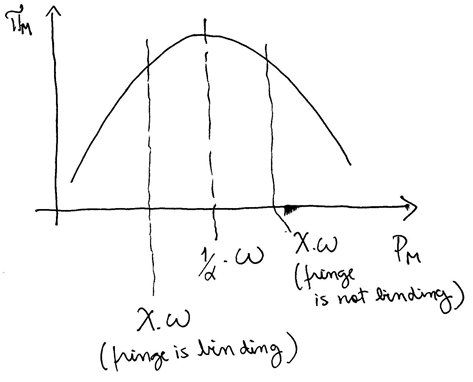
\includegraphics[width=0.7\linewidth]{Imagens/a18i1.png}
\end{figure}

\subsection{\textbf{Notas \% : growth rate in log differences}}

\[
A_t \Rightarrow \gamma \cdot A_t = A_{t+1}
\]

\[
g = \frac{\gamma A - A}{A} = \gamma - 1 \quad \cong
\]

\[
\cong \ln(\gamma \cdot A) - \ln A = \ln \gamma \quad \text{quando } \gamma \cong 1
\]

\subsection{\textbf{Taylor expansion truncada na 1ª ordem:}}

\[
\ln \gamma = \ln 1 + \ln'(1) \cdot (\gamma - 1)
+ \frac{1}{2} \cdot \ln''(1) \cdot (\gamma - 1)^2 + \cdots
\]

\[
= 0 + \frac{1}{1} \cdot (\gamma - 1) = \gamma - 1
\]

\newpage
\section{\textbf{Quality Ladder 2}}
Seja a produção do bem final \(Y_t\) definida por
\[
  Y_t = \Biggl( \sum_{i=1}^m A_{it}^{1-\alpha} x_{it}^{\alpha} \Biggr)^{\!\frac{1}{1-\alpha}}
        \Bigl(\tfrac{L}{m}\Bigr)^{1-\alpha}, \tag{12}
\]
onde \(m\) é o número de bens intermediários, \(x_{it}\) a quantidade do bem \(i\),
\(L\) a população e \(A_{it}\) a qualidade do bem \(i\).

\paragraph{Observação} Diferentemente do modelo de Romer,
\[
Y = L^{1-\alpha}\sum_{i=1}^m x_i^{\alpha},
\]
o produto \textbf{12} não cresce com \(m\). Sob simetria,
\(x_i = X/m\), para todo \(i\), caracterizando um \emph{quality ladder}, e
não uma \emph{variety expansion}.

\begin{align*}
  \frac{\partial Y}{\partial A_i} &> 0, \qquad &&\forall\, i, \\[6pt]
  \frac{\partial Y}{\partial m}   &= 0
  &&\text{(sob simetria).} \ \  \ \textbf{Sob simetria:}
  A_i = A_j = A \quad (\forall\, i,j),
  \qquad
  x_i = \frac{X}{m}.
\end{align*}

\begin{align}
  Y
  &=\Biggl(\sum_{i=1}^{m}
            A^{1-\alpha}\,
            \bigl(\tfrac{X}{m}\bigr)^{\alpha}\Biggr)^{\!\frac{1}{1-\alpha}}
     \Bigl(\tfrac{L}{m}\Bigr)^{1-\alpha} \label{eq:Y_step1}\\[6pt]
  &=\Bigl(m\,A^{1-\alpha}\,X^{\alpha}m^{-\alpha}\Bigr)^{\!\frac{1}{1-\alpha}}
     m^{\,\alpha-1}\,L^{1-\alpha} \label{eq:Y_step2}\\[6pt]
  &=\Bigl(A^{1-\alpha}\,X^{\alpha}\,m^{\,1-\alpha}\Bigr)^{\!\frac{1}{1-\alpha}}
     m^{\,\alpha-1}\,L^{1-\alpha} \label{eq:Y_step3}\\[6pt]
  &=X^{\alpha}\,(A\,L)^{1-\alpha}. \label{eq:Y_final}
\end{align}

A ideia de que uma população maior aumentaria permanentemente o crescimento da PTF tem sido contestada por modelos de crescimento endógeno de segunda geração (ver, por exemplo, Aghion e Howitt, 1998). Em um artigo seminal, Young (1998) argumenta que, à medida que a população cresce, cresce também o número de produtos distintos sobre os quais a pesquisa deve se espalhar. Embora a inovação horizontal ofereça instrumentos para atender a uma variedade de necessidades, ela também aumenta as chances de erros e eleva os custos de informação e transação (ver Aghion e Howitt, 1998).  

Nos modelos schumpeterianos de crescimento endógeno, o efeito líquido sobre o crescimento da proliferação de produtos é zero, enquanto o crescimento da PTF é uma função positiva das inovações verticais que aumentam a qualidade dos produtos (Young, 1998; Aghion e Howitt, 1998). Aghion e Howitt (1998) sugerem usar a população ou os insumos de trabalho para filtrar as inovações horizontais das verticais, sob a suposição de que as inovações horizontais aumentam proporcionalmente à população ou aos insumos de trabalho.

O bem final é usado p/ 3 finalidades: consumo, pesquisa e produção de (conversão em) bens intermediários.

Uma inovação bem-sucedida na seção \(i\) fará com que
\[
A_{it} = \gamma\,A_{i,t-1},
\]
como antes na versão \textit{Toy}.

\begin{itemize}
  \item A atividade de pesquisa é caracterizada por: se \(N_{it}\) unidades do bem final são investidas no setor \(i\) no início do período \(t\), então o potencial inovador \(i\) terá sucesso com probabilidade
    \[
      \underbrace{\mu_{it}}_\text{probabilidade de sucesso} = \lambda\,f(n_{it}), \quad f'(n)>0,\; f(0)=0,\; \underbrace{f''(n)<0}_\text{função côncava}
      \tag{13}
    \]
    \begin{itemize}
      \item onde \(n_{it} \equiv \frac{N_{it}}{\underbrace{\gamma\,A_{i,t-1}}_\textit{target}}\) é o gasto(em dólar por exemplo) com P\&D ajustado pela produtividade;
      \item Note que, conforme \(A_{i}\) cresce ao longo do tempo, um mesmo \(N_{i}\) (investimento no setor \(i\)) é cada vez menos efetivo \(\to\) \emph{fishing‐out effect}.
    \end{itemize}
  \item Assumindo que todas as possibilidades de duplicação de esforços de pesquisa no setor \(i\) já estão incorporadas (sendo levadas em conta) pela concavidade da função \(f\) em (13), segue‐se que\ldots
\end{itemize}

\(A_{it} = 
\begin{cases}
\gamma\,A_{i,t-1}, & \text{com probabilidade } \lambda\,f(n_{it}),\\
A_{i,t-1},         & \text{com probabilidade } 1 - \lambda\,f(n_{it}) \ \ 
\end{cases}
\) 

Essa distribuição de probabilidades é a equação \textbf{(14)}

Definindo, usualmente,  
\[
g_i \equiv \frac{\mathbb{E}(A_{it}) - A_{i,t-1}}{A_{i,t-1}}
\tag{15}
\]

Das expressões (14) e (15) segue-se que  
\[
g_i = \underbrace{\lambda\,f(n_i)}_\text{frequência das inovações}\,\underbrace{(\gamma - 1)}_\text{salto das inovações}
\tag{16}
\]

Agregação (dos setores \(i\) para a economia como um todo) \(\leftrightarrow\) ideia de “setor representativo”:  \begin{itemize}
    \item \(\text{Agregação (simetria):} \ \forall\,\underbrace{i,j}_\text{setores}, t\to\infty:A_{it}\approx A_{jt}\)
    \item \(A_{it}=\underbrace{A_{i,0}}_1\gamma^{j_i}\), onde \(j_i\equiv\)números de sucessos no setor \(i \ \ , \ \ 0<j_i<1\)
    \item Pode-se mostrar que  
    \[
      \frac{\mathrm{desv.pad.}(A_{it})}{\mathbb{E}(A_{it})} \;\longrightarrow\; 0
      \quad(t\to\infty).
    \]  
    \item Ou seja, no longo prazo todos os setores estarão com o mesmo \(A\) — todos desfrutarão da mesma probabilidade de inovação e intensidade de investimento, por simetria na função de produção (12).
\end{itemize}

Logo,  
\[
g = \lambda\,f(n)\,(\gamma - 1)
\tag{16$'$}
\]

Condição de não-arbitragem em pesquisa: custo de investir 1 unidade (\(N=1\)) de bem final em P\&D = retorno esperado de 1 período:  
\[
\underbrace{1}_\text{numerário} = \lambda\,f'(n) \frac{\partial n}{\partial N} \underbrace{\pi}_\text{lucro de 1 periódo}=\lambda\,f'(n)\,\underbrace{\frac{\pi}{\gamma\,A_{t-1}}}_\textit{productivity adjusted monopoly rent}  
\tag{17}
\]

Suponha que o inovador bem-sucedido seja capaz de produzir a última geração do bem intermediário a uma proporção 1 unidade de bem final:1 unidade de bem intermediário, e que ele se defronta com uma margem de imitadores capazes de fazer o mesmo a um custo de \(\chi\) unidade de bem final:1 unidade de bem intermediário. Então,  
\[
\tilde\pi = (p - 1)\,x = (\chi - 1)\,x
\tag{18}
\]

Derivando a equação \textbf{12},em função de \(x\), temos:
\[
\frac{\partial Y}{\partial x}=\alpha A^{1-\alpha}x^{\alpha-1}(\frac{L}{m})^{1-\alpha}
\]

Por outro lado, defrontando-se com \(p=\chi\) pelo bem intermediário, os produtores de bem final demandarão uma quantidade \(x\) de intermediário tal que  
\[
\chi = 2\frac{Y}{2x} = \alpha\Bigl(\tfrac{m\,x}{A\,L}\Bigr)^{\alpha-1}
\tag{19}
\]

Substituindo (19) em (18) vem  
\[
\tilde\pi = \gamma(\chi)\,\frac{A\,L}{m}
\tag{20}
\]

onde
\[
\gamma(X) = (X - 1)\,\Bigl(\tfrac{X}{\alpha}\Bigr)^{\frac{1}{\alpha - 1}};\quad \gamma'(X) > 0
\tag{21}
\]

Agora, levando em conta que na eq. de arbitragem em pesquisa (17) deve ser \(\gamma\,A_{t-1} = A_{t}\), já que o monopolista é alguém que acabou de inovar, e substituindo (20) em (17), vem
\[
1 = \underbrace{\underbrace{\lambda\,f'(n)}_{Probabilidade \ Marginal}\,\underbrace{\gamma(\overset{+}{\chi})}_{Poder \  de \  Monopolio}\,\underbrace{\frac{L}{m}}_{Market-Share}}_{RME\text{(Retorno Marginal Esperado)}}=\textbf{RME}(\overset{+}{\chi},\overset{-}{n})
\tag{17$'$}
\]

A expressão (17$'$) pode ser resolvida para \(n\). Daí, substituindo essa solução em (16$'$), obtemos a taxa de crescimento esperado da produtividade, que também é aproximadamente igual à taxa de crescimento do produto per capita nesse modelo. Por ex., adotando a forma funcional
\[
f(n) = \sqrt{2}\,n.
\]

P/ descrever a tecnologia de pesquisa, tem-se que
\[
g = \lambda^{2}\,\delta(\chi)\,\Bigl(\tfrac{L}{m}\Bigr)\,(\gamma-1)
\tag{22}
\]

\noindent\textbf{Notas.}\quad\(\to\) número de inovações bem-sucedidas  
\[
A_{t} = A_{0}\,\gamma^{j},\quad 0 \le j \le t
\]
Onde \(j\) é o número de inovações bem-sucedidas
\[
\ln A_{t} = \ln A_{0} + j\,\ln\gamma.
\]
Suponha que cada inovação tenha distribuição de Bernoulli c/ probabilidade \(\mu\). Então \(j\) é uma binomial \(\mathrm{Bin}(t,\mu)\).

\[
\mathbb{E}[\ln A_{t}] = \ln A_{0} + \underbrace{\mu\,t}_{E(j)}\,\ln\gamma.
\]
Normalizando \(A_{0}=1\), tem-se
\[
\mathbb{E}[\ln A_{t}] = \mu\,t\,\ln\gamma.
\]
\[
\operatorname{Var}[\ln A_{t}]
= (\ln\gamma)^{2}\,\mu\,(1-\mu)\,t.
\]
\[
\text{desv.\,pad.}(\ln A_{t})
= \ln\gamma\;\sqrt{\mu\,(1-\mu)\,t}.
\]
\[
\frac{\text{desv.\,pad.}(\ln A_{t})}{\mathbb{E}[\ln A_{t}]}
= \frac{\sqrt{1-\mu}}{\sqrt{\mu}\,\sqrt{t}}
\quad\Longrightarrow\quad
\lim_{t\to\infty}
\frac{\text{desv.\,pad.}(\ln A_{t})}{\mathbb{E}[\ln A_{t}]}
= 0.
\]

\newpage
\section{\textbf{Quality Ladder 3}}

\textbf{Aplicação do modelo num cenário internacional}

\begin{itemize}
    \item \textit{“catch-up tecnológico”} (salto tecnológico) se tornou uma hipótese:  
          O país pobre alcançar o país rico
\end{itemize}

\begin{itemize}
    \item uma aplicação : transferência internac.\ de tecnologia e \textit{convergence clubs} 
\end{itemize}

\noindent O conhecimento, de alguma forma “vaza” do país rico para o país pobre.\\
Obs: lembrar dos grupos de convergência

\begin{itemize}
    \item spillovers (vazamentos) internacionais de conhecimento a nível setorial.  
          Quando um setor atrasado em um país em desenv.\ sofre inovação, ele salta p/ a fronteira tecnológica mundial.  
          Portanto, quanto $>$ o atraso, maior o salto ou tamanho das inovações e, portanto, $>$ a tx.\ de crescimento p/ uma dada frequência (ou esforço) de inovação $\Longrightarrow$ força pró-convergência
    \item na verdade, os países atrasados fazem uma atividade de
          \textbf{implementação} e \textbf{adaptação}, e não P\&D propriamente.
\end{itemize}

Contudo, por apresentar características semelhantes (absorver recursos reais, $K_{\text{humano}}$, ter resultados incertos), produzin


\;Ver Mayer–Foulkes (2002), pág.\ 3 $\langle\;\rangle$


\textbf{CANAIS DE TRANSFERÊNCIA DE TECNOLOGIA}

\begin{itemize}
    \item Comércio Internacional
    \item Licensing (OEM) $\leftrightarrow$ Royalties
    \item Investimento direto estrangeiro (FDI) $\leftarrow$ multinacionais
\end{itemize}

$\uparrow$ nível tecnológico, etc.), essa implementação e adaptação será modelada
analiticamente igual a P\&D.

\[
A_{t-1} \;\equiv\; \text{nível da tecnologia num certo país no período } t-1
\]

\[
\overline{A}_{t-1} \;\equiv\; \text{fronteira mundial de tecnologia no período } t-1,
\]
\[
\text{com}\;
\overline{A}_{t-1}= \max_{j=1,\dots,h}\!\bigl\{A_{t-1}^{\,j}\bigr\},
\; h\text{ países no mundo}
\]

Então, uma inovação bem-sucedida nesse certo país faz c/ que

\[
A_{t} = \delta\,\overline{A}_{t-1}
\]

Assim, a produtividade doméstica num típico setor intermediário evolui de acordo c/

\[
\ln A_{t} =
\begin{cases}
\ln A_{t-1} + \ln\delta, & \text{c/ probab. } \mu\\[4pt]
\ln A_{t-1}, & \text{c/ probab. } 1-\mu
\end{cases}
\tag{23}
\]

\noindent\footnotesize Comparar com o \emph{Quality ladder 2} (economia fechada) $\rightarrow$ equação 14 —
$\Rightarrow$ hipótese de \emph{catch-up}\normalsize


onde $\mu = \chi\,f(n)$, como antes, somente que

\[
n \;=\; \frac{N_c}{\delta\,\overline{A}_{t-1}}
\tag{24}
\]

pois o \emph{targeting} é feito sobre $\delta\,\overline{A}_{t-1}$.

Comparar com \emph{quality ladder 2}.  
É possível notar que, para ter o mesmo $n$, o $N$ precisa ser maior em economia aberta,
pois queremos melhorar a fronteira mundial.  
Portanto, é muito mais caro fazer P\&D em eco aberta.


Por outro lado, a fronteira mundial se move c/ inovação em qualquer país, i.e.,

\[
\ln \overline{A}_{t} =
\begin{cases}
\ln \overline{A}_{t-1} + \ln\delta, & \text{c/ probab. } \widebar{\mu}\\[4pt]
\ln \overline{A}_{t-1}, & \text{c/ probab. } 1-\widebar{\mu}
\end{cases}
,
\qquad
\widebar{\mu} \;=\; \sum_{j=1}^{h} \gamma_{j}\,f(n_{j})
\tag{25}
\]

\noindent obs.: note que, na formulação de $\widebar{\mu}$, supõe-se não ocorrer duplicação de
resultados de pesquisa internacionalmente.


Por (25), a tx.\ de crescimento da produtividade mundial, medida como uma diferença em logs, é

\[
\overline{g} \;=\; \widebar{\mu}\,\ln\delta
\tag{26}
\]

Supor não haver comércio internac.\ em bens interm.; temos que os custos e benefícios de P\&D são iguais a antes, c/ exceção do \emph{targeting}: $\delta A_{t-1}$ e não $\overline{A}_{t-1}$.  
Dessa forma, o “salto de produtividade” decorrente de uma inovação é dado por
\[
\ln A_{t}(\text{inov.})-\ln A_{t-1}
   =\ln\overline{A}_{t-1}+\ln\delta-\ln A_{t-1}
   =\ln\delta+d_{t-1},
\qquad
d_{t-1}\equiv\ln\overline{A}_{t-1}-\ln A_{t-1}
\tag{27}
\]
(\emph{medida de “distância da fronteira”})

Logo, a tx.\ média de crescimento da produtividade do nosso país será
\[
g_{t}=\mu\bigl(\ln\delta+d_{t-1}\bigr)
\tag{28}
\]

Por sua vez, $d$ evolui conforme
\[
d_{t}=
\begin{cases}
d_{t-1}, & \text{c/ probab.\ }1-\bar{\mu}\\[4pt]
0,       & \text{c/ probab.\ }\mu\\[4pt]
\ln\delta+d_{t-1}, & \text{c/ probab.\ }\bar{\mu}-\mu
\end{cases}
\tag{29}
\]
(\emph{alguém no mundo inovou, mas não foi no país doméstico})

Logo, a distância esperada é
\[
\hat{d}_{t}
=(1-\bar{\mu})d_{t-1}+(\bar{\mu}-\mu)(\ln\delta+d_{t-1})
=d_{t-1}+(\bar{\mu}-\mu)\ln\delta-\mu d_{t-1}
=(1-\mu)d_{t-1}+(\bar{\mu}-\mu)\ln\delta
\tag{30}
\]

A expr.\ (30) é estável se $\mu>0\Longrightarrow\hat{d}_{t}=\hat{d}_{t-1}$ em \emph{steady-state}.  
Aplicando (30):
\[
\hat{d}_{t}=(1-\mu)\hat{d}_{t}+(\bar{\mu}-\mu)\ln\delta
\Longrightarrow
\hat{d}_{t}=\dfrac{\bar{\mu}-\mu}{\mu}\,\ln\delta
\tag{31}
\]

Ora, uma distância estável significa que o país cresce à mesma tx.\ que a fronteira, i.e.\ $g_{\text{país}}=\bar{g}$.

Mas, se $\mu=0$ (i.e.\ em equilíbrio $n=0$), então a distância cresce sem limite $\Longrightarrow$ \emph{divergência}: $g=0<\bar{g}$.

Quando pode ocorrer $\mu=0$, i.e.\ $n=0$?  
Considere novamente
\[
1=\lambda\,f'(n)\,\delta(X)\,\frac{L}{m}
\tag{17$'$}\quad\text{(research arbitrage condition)}
\]

Como $f''<0$, se $f'(0)=+\infty$, sempre haverá $n^{\ast}$ solução p/ (17$'$).  
Mas suponha $f'(0)<\infty$; então pode ocorrer
\[
1>\lambda\,f'(0)\,\delta(X)\,\frac{L}{m},
\]
ou seja, os custos de pesquisa excedem os retornos para qualquer $n>0$, implicando $n^{\ast}=0$.


Assim, uma condição necessária e suficiente p/ $n^{\ast}>0$ é
\[
1<\lambda\,f'(0)\,\delta(X)\,\frac{L}{m}
\;\Longrightarrow\;
\lambda\,\delta(X)\,\frac{L}{m}>\frac{1}{f'(0)}
\tag{32}
\]

Conclusões: nosso país estagnará $(n=0,\;g=0)$ se …
\begin{itemize}
  \item a pesquisa for muito improdutiva ($\uparrow$~custo / baixo ganho);
  \item direitos de propr.\ intelectual forem baixos ($\chi$ pequeno);
  \item nível de capital humano/educação for reduzido ($L$ pequeno).
\end{itemize}

\noindent Contudo, basta um $n>0$, por menor que seja, para o país crescer à taxa\ mundial $\bar{g}$ no longo prazo.

\begin{figure}[H]
    \centering
    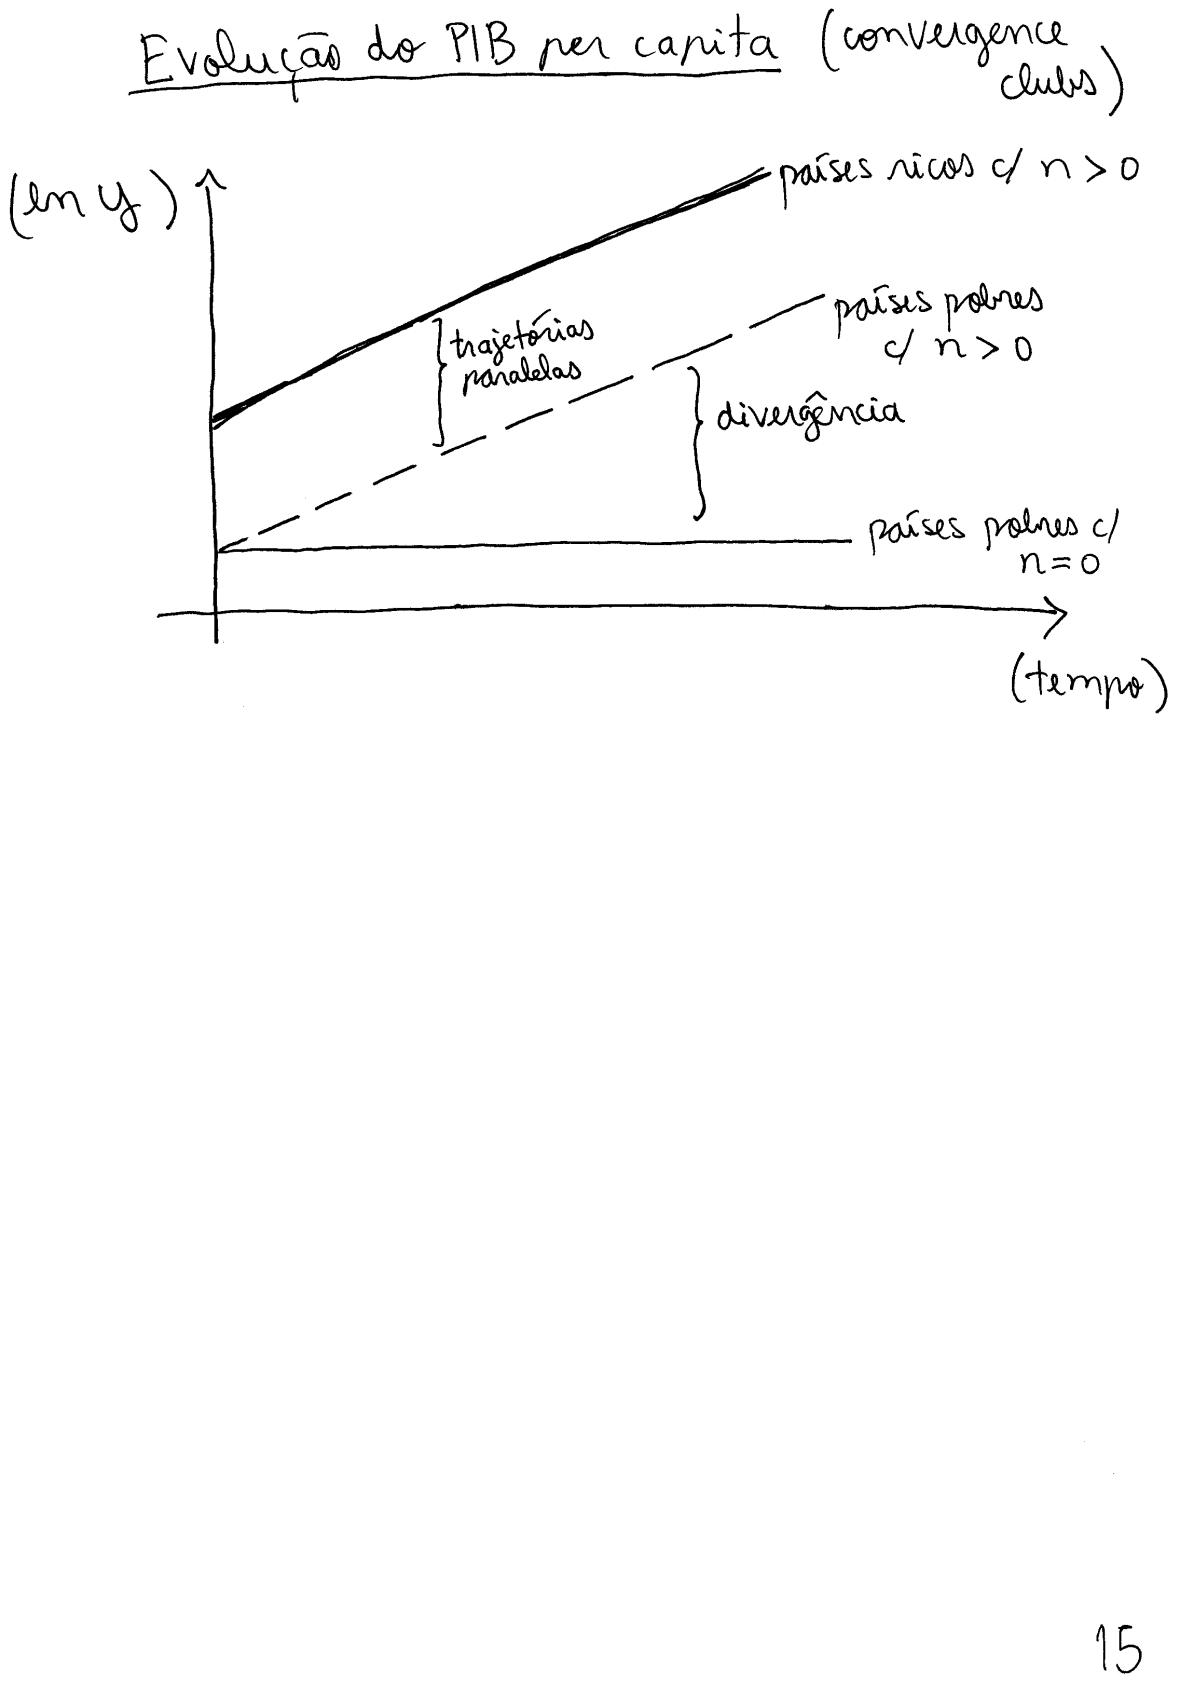
\includegraphics[width=0.7\linewidth]{Imagens/a19i1.png}
\end{figure}

\newpage
\section{\textbf{Financial Development}}

\begin{figure}[H]
    \centering
    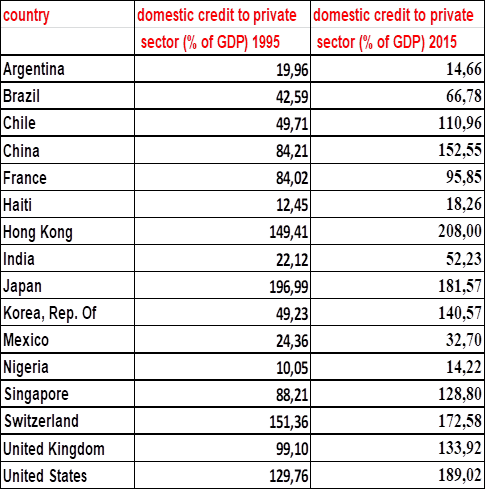
\includegraphics[width=0.7\linewidth]{Imagens/a20i1.png}
\end{figure}

\textbf{Fonte}:\url{FONTE:http://data.worldbank.org/indicator/FS.AST.PRVT.GD.ZS}

\begin{figure}[H]
    \centering
    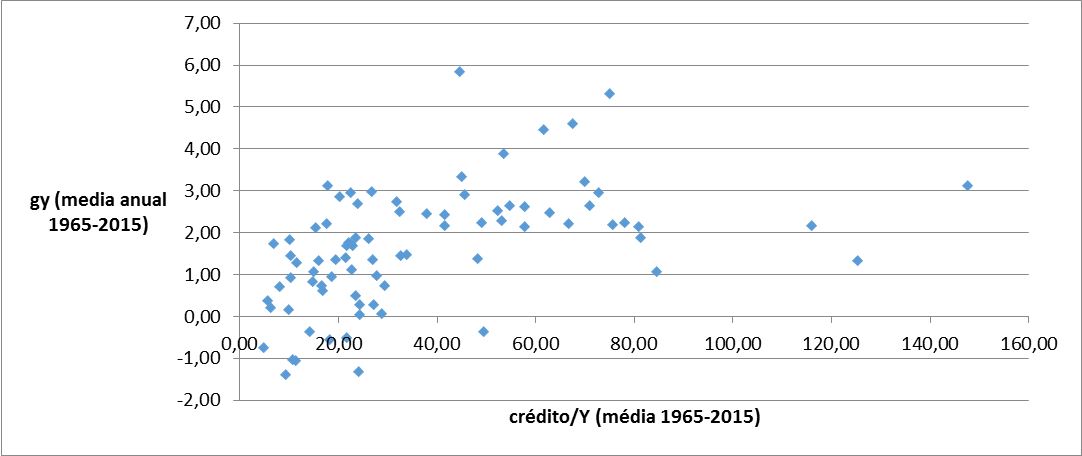
\includegraphics[width=0.7\linewidth]{Imagens/a20i2.png}
\end{figure}

\textbf{Fonte}\url{http://data.worldbank.org/indicator/FS.AST.PRVT.GD.ZS}


\textbf{Transferência internacional de tecnologia como força pró-convergência}

\begin{itemize}
    \item A transferência internacional de tecnologia é uma poderosa força pró-convergência: se um país ``atrasado’’ possuir um nível mínimo de capital humano e de direitos de propriedade intelectual (IPRs) que viabilize algum investimento em P\&D (por menor que seja), esse país alcançará, no longo prazo, a mesma taxa de crescimento da fronteira tecnológica.
\end{itemize}

\begin{itemize}
    \item Três componentes-chave da teoria do \textit{desenvolvimento financeiro}:
          \begin{itemize}
              \item \textbf{i)} \textit{Custo de transferência/absorção de tecnologia}.  
                    O custo, análogo ao de P\&D, cresce mais do que proporcionalmente com a probabilidade de dar um salto tecnológico:
                    \[
                        \mu(n)=\lambda\,f(n), \qquad f'>0,\;f''<0.
                    \]
              \item \textbf{ii)} \textit{“Fishing-out effect”}.  
                    Com o tempo,
                    \[
                        n_t=\frac{N_t}{\delta\,A_{t-1}},
                    \]
                    de modo que, à medida que $A\uparrow$, é necessário um $N$ cada vez maior para manter o mesmo $n$ (e, portanto, a mesma $\mu$).
              \item \textbf{iii)} \textit{Imperfeição no mercado de crédito} (para projetos de P\&D).  
                    Um inovador pode fraudar seus credores a um custo que cresce com o grau de desenvolvimento financeiro do país.  Assim,
                    \[
                        N_i = M^{+}(c_i)\,\omega_i^{+}(A_i), \tag{1}
                    \]
                    em que $M(c_i)$ é o \emph{credit multiplier} e $\omega_i(A_i)$ o salário do inovador.  
                    Em geral, $N_i < N_i^{\ast}$, onde $N_i^{\ast}$ é o nível ótimo (não-restringido) de investimento derivado da condição de não-arbitragem em pesquisa.
          \end{itemize}
\end{itemize}

\noindent Inspeccionando (1), obtêm-se as implicações:

\begin{itemize}
    \item[(a)] Para um mesmo $A$, um custo $c$ maior implica maior crescimento $\;\Longrightarrow\;$ \textit{financial development policies};
    \item[(b)] Para um mesmo $c$ (logo mesmo $M$), quanto menor $A$, menores $\omega$ e $N$ $\;\Longrightarrow\;$ desvantagem para países retardatários (\textit{``laggard countries''}), contrabalançando o \textit{efeito Gerschenkron} de \textit{catch-up} ($A_{t-1}\rightarrow\overline{A}_{t}$): quanto mais atrasado o país $i$, maior o salto tecnológico.
\end{itemize}

\textbf{O Modelo}

\begin{itemize}
    \item \textit{Indivíduos e preferências}.  
          População de tamanho $L\rightarrow1$ (normalização), de modo que quantidades agregadas e \emph{per capita} coincidem:
          \[
              U = c_{1} + \beta\,c_{2}, \qquad 0<\beta<1.
          \]
          Cada indivíduo vive dois períodos, recebendo $2$ unidades de trabalho no 1º período e $0$ no 2º.
\end{itemize}


\begin{itemize}
    \item the multi-purpose general good, used for consumption, as input to R\&D and as an input to produce intermediate goods.
\end{itemize}

\[
    Z_t
      = L^{1-\alpha}\!
        \int_{0}^{1} A_t(i)^{\,1-\alpha}\,x_t(i)^{\,\alpha}\,di,
    \qquad 0<\alpha<1
    \tag{1}
\]

(\emph{set } $L=1$):
\[
    Z_t
      = \int_{0}^{1} A_t(i)^{\,1-\alpha}\,x_t(i)^{\,\alpha}\,di
    \tag{1'}
\]

Fazendo o preço igual ao valor do produto marginal para o bem intermediário $i$ e tomando $Z$ como numerário ($P_Z=1$),
\[
    P_t(i)
      = \alpha\!\left(\frac{x_t(i)}{A_t(i)}\right)^{\alpha-1}
    \tag{2}
\]

Supondo, como nos modelos anteriores, que há uma margem de imitadores capazes de produzir $1$ un.\ de $i$ com $\chi$ un.\ de $Z$, de modo que
\[
    P_t(i)=\chi
    \tag{2'}
\]

Igualando \textbf{2} e \textbf{2'},
\[
    x_t(i)
      = \left(\frac{\alpha}{\chi}\right)^{\frac{1}{1-\alpha}} A_t(i)
    \tag{3}
\]

\subsection{\textbf{Processo de inovação}}

Um inovador bem-sucedido em $t-1$ torna-se monopolista em $t$, na indústria $i$, com probabilidade $\mu_t(i)$:
\[
    A_t(i)=
    \begin{cases}
        \overline{A}_t,   & \text{com probab.\ }\mu_t(i),\\[6pt]
        A_{t-1}(i),       & \text{com probab.\ }1-\mu_t(i)
    \end{cases}
    \tag{4}
\]

$\overline{A}_t$ é a fronteira tecnológica mundial (com $\displaystyle\lim_{t\to\infty}\frac{A_t(i)-A_t(j)}{A_t(j)}=0$), crescendo a taxa constante $g$ (exógena por enquanto).

O lucro de uma firma monopolista é
\[
    \Pi_t^{\,i}
      = (\chi-1)\,x_t(i)
      \stackrel{(3),(4)}{=}
        \Pi\,\overline{A}_t,
    \qquad
    \Pi\equiv(\chi-1)
          \left(\tfrac{\alpha}{\chi}\right)^{\frac{1}{1-\alpha}}.
\]

\subsection{\textbf{Aggregate behavior}}

Defina a \emph{produtividade média} da economia:
\[
    A_t \equiv \int_{0}^{1} A_t(i)\,di.
\]

Substituindo \textbf{3} em \textbf{1'} obtém-se
\[
    Z_t
      = \xi\,A_t,
    \qquad
    \xi \equiv \left(\tfrac{\alpha}{\chi}\right)^{\frac{\alpha}{1-\alpha}}.
\]

A dinâmica de $A_t$ é
\[
    A_t
      = \mu_t\,\overline{A}_t + (1-\mu_t)\,A_{t-1}.
    \tag{5}
\]

Produtividade normalizada:
\[
    a_t \equiv \frac{A_t}{\overline{A}_t},
    \qquad
    \ln(a_t)^{-1}= \ln\overline{A}_t - \ln A_t,
\]
onde $a_t$ é a medida inversa da \emph{distância à fronteira} (gap tecnológico).

Dividindo \textbf{5} por $\overline{A}_t$ e usando $\overline{A}_t=(1+g)\overline{A}_{t-1}$:
\[
    a_t
      = \mu_t + \frac{1-\mu_t}{1+g}\,a_{t-1}.
    \tag{5'}
\]

Como o setor \emph{general purpose} é competitivo,
\[
    w_t
      = \frac{\partial Z_t}{\partial L_t}
      = (1-\alpha)L^{-\alpha}\!\int_{0}^{1} A_t(i)^{1-\alpha}\,x_t(i)^{\alpha}di
      \stackrel{L=1}{=}
        (1-\alpha)Z_t
      = (1-\alpha)\,\xi\,A_t.
    \tag{6}
\]
Assim, $w_t$ é proporcional a $A_t$.

Identidade de produto/renda per capita:
\[
    Y_t
      \;\equiv\;
      w_t L_t + \mu_t \Pi_t
      = (1-\alpha)\,\xi\,A_t
      + \mu_t\,\Pi\,\overline{A}_t.
    \tag{7}
\]

\subsection{\textbf{Tecnologia de inovação}}

\[
    N_{t-1}
      = \tilde{N}(\mu_t)\,\overline{A}_t
      = \bigl(\eta\,\mu_t + \delta\tfrac{\mu_t^{2}}{2}\bigr)\,\overline{A}_t.
    \tag{8}
\]

São as unidades do bem que devem ser investidas em P\&D para inovar com probabilidade $\mu_t$.
De \textbf{8},
\[
    \mu_t
      = \frac{\sqrt{\eta^{2}+2\delta\,\tfrac{N_{t-1}}{\overline{A}_t}}-\eta}{\delta}
      \;=\;
      f\!\bigl(N_{t-1},\overline{A}_t\bigr),
\]
com \(\partial\mu_t/\partial N_{t-1}>0\), \(\partial\mu_t/\partial\overline{A}_t<0\) e \(\partial^{2}\mu_t/\partial N_{t-1}^{2}<0\).

Em equilíbrio, $\mu_t$ maximiza o \emph{profit} líquido:
\[
    \beta\,\mu_t\,\Pi\,\overline{A}_t
      -\tilde{N}(\mu_t)\,\overline{A}_t,
    \tag{9}
\]
onde $\beta$ desconta o lucro ao valor presente (visão de $t-1$).

\noindent\emph{Questão:} será que \textbf{9} é maximinizada \textit{globalmente} ou sujeita a restrições (de crédito)?

%--------------------------------------
\subsubsection{\textbf{Perfect credit markets}}
\begin{itemize}
    \item \emph{Hipóteses}:  
          \begin{itemize}
              \item crédito ilimitado (em quantidade);  
              \item compromisso vinculante de reembolso.
          \end{itemize}
          Nessas condições, a escolha de $\mu$ é interior: $\mu_t=\mu^{\ast}$, com
          \[
              \tilde N'(\mu^{\ast})=\beta\,\Pi
              \;\Longrightarrow\;
              \eta+\delta\,\mu^{\ast}= \beta\,\Pi
              \;\Longrightarrow\;
              \boxed{\mu^{\ast}= \dfrac{\beta\,\Pi-\eta}{\delta}}.
          \]
    \item O dispêndio ótimo em P\&D é
          \[
              N_{t-1}^{\ast}= n^{\ast}\,\overline{A}_t,
              \qquad
              n^{\ast}= \tilde N(\mu^{\ast})
                      =\frac{\beta^{2}\Pi^{2}-\eta^{2}}{2\delta}
              \quad\text{[via (8)]}.
          \]
    \item Pelo \textbf{5'} o \emph{gap} tecnológico evolui segundo
          \[
              a_{t+1}= \mu^{\ast}
                      + \frac{1-\mu^{\ast}}{1+g}\,a_t
                      \;\equiv\;F_{1}(a_t). \tag{10}
          \]
          No longo prazo
          \[
              a^{\ast}= \frac{(1+g)\,\mu^{\ast}}{g+\mu^{\ast}}\;\in\;(0,1).
          \]
\end{itemize}

\paragraph{Renda de \emph{steady‐state}.}
Da identidade \textbf{7},
\[
    Y_t^{\ast}
      = \Bigl[(1-\alpha)\,\xi\,a^{\ast}
              +\mu^{\ast}\,\Pi\Bigr]\,
        \overline{A}_t.
    \tag{11}
\]
\begin{itemize}
    \item[Obs.~1)] Como $N_{t-1}^{\ast}=n^{\ast}\,\overline{A}_t$, $N$ cresce à mesma taxa $g$ que $\overline{A}$; logo $N/Y$ é constante no \emph{steady‐state}.
    \item[Obs.~2)] Países sem restrição de crédito convergem para a mesma taxa $g$, mas diferenças internacionais em $\Pi$ (dependentes de $\chi$ ou de IPRs) geram níveis distintos de $Y$ $\Rightarrow$ \textit{parallel growth paths}.
\end{itemize}

%--------------------------------------
\subsubsection{\textbf{Credit constraints}}

Para investir $N_t$ num projeto de P\&D, o potencial inovador toma empréstimo
\[
    D_t = N_t - w_t,
\]
onde $w_t$ é o seu salário.  
O contrato de crédito depende do estado da natureza:  

\begin{itemize}
    \item \textit{sucesso} $\Rightarrow$ paga $D_t$ ao credor;
    \item \textit{fracasso} $\Rightarrow$ paga $0$.
\end{itemize}

\paragraph{Fraude ex ante.}
Se, a um custo proporcional $c\,N_t$ ($0<c<1$), o inovador conseguir esconder o sucesso, ele frauda quando
\[
    \underbrace{c\,N_t}_{\text{custo de fraude}}
      < \underbrace{\tilde{\mu}\!\Bigl(\tfrac{N_t}{\overline{A}_{t+1}}\Bigr)\,
                    R\,(N_t-w_t)}_{\text{valor esperado do calote}},
    \tag{12}
\]
onde $R\equiv1+r$ é o fator de juros.  
A condição \textbf{12} (com sinal $\ge$) é chamada por AHKM–F de \emph{incentive-compatibility constraint}; fraude ocorre quando ela é violada.

\paragraph{Não‐arbitragem do credor.}
Se o credor pode aplicar num título \emph{riskless} à taxa $r$,
\[
    \boxed{\tilde{\mu}\!\Bigl(\tfrac{N_t}{\overline{A}_{t+1}}\Bigr)\,R = 1+r.}
    \tag{13}
\]
Como a inovação é incerta, $R=(1+r)/\tilde{\mu}>1+r$.

\medskip
Juntando \textbf{12} e \textbf{13} obtém‐se a \textbf{restrição de crédito}
\[
    \boxed{N_t \le \frac{1+r}{1+r-c}\;w_t}
    \tag{14$'$}
\]
(\emph{credit multiplier}, crescente em $c$).  
Ela é \emph{binding} quando impede o nível ótimo $N_t^{\ast}=n^{\ast}\,\overline{A}_{t+1}$, ou seja
\[
    N_t = \frac{1+r}{1+r-c}\;w_t
          < n^{\ast}\,\overline{A}_{t+1}.
    \tag{15}
\]
Substituindo $w_t=(1-\alpha)\,\xi\,A_t$ [eq.\ (6)] em \textbf{15},
\[
    \frac{A_t}{\overline{A}_t}
      < n^{\ast}\,(1+g)\,
        \frac{1+r-c}{1+r}\,
        \frac{1}{(1-\alpha)\,\xi}
      \quad\Longrightarrow\quad
      a_t<\text{(limite)}.
    \tag{16}
\]
\begin{itemize}
    \item Conclusão: um país investirá \emph{menos} que a taxa ótima quando
          \begin{itemize}
              \item $a_t$ for pequeno (grande distância da fronteira); \textbf{ou}
              \item $c$ for pequeno (baixo desenvolvimento financeiro).
          \end{itemize}
\end{itemize}

\paragraph{Probabilidade de inovação com restrição.}
Com \textbf{14$'$} e $\overline{A}_{t+1}=(1+g)\,\overline{A}_t$,
\[
    n_t
      \equiv \frac{N_t}{\overline{A}_{t+1}}
      = \frac{1+r}{1+r-c}\;
        \frac{(1-\alpha)\,\xi}{1+g}\;
        a_t
      \;\equiv\; \omega(c)\,a_t,
\]
onde $\omega(c)$ destaca o papel do sistema financeiro.

A probabilidade de inovação é, então,
\[
    \tilde{\mu}\bigl(\omega(c)\,a_t\bigr)=\mu_{t+1}
    \qquad(\text{pois, via (8), o investimento em }t
    \text{ pode gerar inovação em }t\!+\!1).
\]
Logo, usando \textbf{5'},
\[
    a_{t+1}
      = \tilde{\mu}\!\bigl(\omega(c)\,a_t\bigr)
        + \frac{1-\tilde{\mu}\!\bigl(\omega(c)\,a_t\bigr)}{1+g}\,a_t
      \;\equiv\; F_{2}(a_t).
    \tag{17}
\]
\emph{Observação}: comparando \textbf{17} com \textbf{10}, é claro que
$\tilde{\mu}\bigl(\omega(c)\,a_t\bigr)<\mu^{\ast}$;  
a restrição de crédito retarda a convergência.

%--------------------------------------------------
% Continuação — Dinâmica sob restrição de crédito
%--------------------------------------------------

\paragraph{Probabilidade de inovação com restrição revisitada.}

Da restrição de crédito \textbf{14$'$} e do fato de $\overline{A}_{t+1}=(1+g)\,\overline{A}_t$, definimos

\[
    n_t
      \;\equiv\;
      \frac{N_t}{\overline{A}_{t+1}}
      \;=\;
      \frac{1+r}{1+r-c}\;
      (1-\alpha)\,\xi\;
      \frac{A_t}{\overline{A}_{t+1}}
      \;=\;
      \frac{1+r}{1+r-c}\;
      \frac{(1-\alpha)\,\xi}{1+g}\;
      a_t
      \;\equiv\;
      \omega(c)\,a_t,
    \tag{17}
\]

onde $\displaystyle \omega(c)=\frac{1+r}{1+r-c}\,
            \frac{(1-\alpha)\,\xi}{1+g}>0$.

Resumindo, a probabilidade de inovação \emph{efetiva} em $t+1$ é
\[
    \tilde{\mu}\bigl(\omega(c)\,a_t\bigr)=\mu_{t+1},
\]
e, usando \textbf{5$'$}, a dinâmica da razão $a_t$ obedece a

\[
    a_{t+1}
      \;=\;
      \tilde{\mu}\!\bigl(\omega(c)\,a_t\bigr)
      + \frac{1-\tilde{\mu}\!\bigl(\omega(c)\,a_t\bigr)}{1+g}\,a_t
      \;\equiv\;
      F_{2}(a_t).
    \tag{18}
\]

Comparando \textbf{18} com \textbf{10}, vê-se que
$\tilde{\mu}\bigl(\omega(c)\,a_t\bigr)<\mu^{\ast}$:  
uma \emph{economia credit constrained} converge mais lentamente.

\paragraph{Limite de crédito e limiar de atraso.}

Com $\omega(c)$, a condição \textbf{16} torna-se

\[
    a_t < \frac{n^{\ast}}{\omega(c)}
        \;\equiv\;
        \bar{a}(c),
    \tag{16$'$}
\]

isto é, só quando o atraso é suficientemente grande ($a_t<\bar a(c)$)
a restrição de crédito é \emph{binding} e a economia segue a trajetória
$F_{2}$.  Caso contrário ($a_t\ge\bar a(c)$) ela opera no regime
\textit{não} restringido, seguindo $F_{1}$.

No geral, portanto,
\[
    a_{t+1}=F(a_t)=\min\bigl\{F_{1}(a_t),\,F_{2}(a_t)\bigr\}.
\]

\begin{itemize}
    \item[(i)] $F_{1}(a_t)$ é linear, com intercepto positivo
          $F_{1}(0)>0$ e inclinação constante
          $F_{1}'=\dfrac{1-\mu^{\ast}}{1+g}>0$.
    \item[(ii)] Economias com $c$ \emph{alto} têm
          limiares $\bar{a}(c)$ mais baixos, entrando
          mais cedo no regime de investimento ótimo.
\end{itemize}

\paragraph{Derivadas iniciais de $F_{2}$.}

Para $n\equiv\omega(c)\,a_t$:

\[
    \mu(n)
      =\frac{\sqrt{\eta^{2}+2\delta\,n}\;-\eta}{\delta},
    \quad
    \mu(0)=0,
    \qquad
    \mu'(0)=\frac{1}{\eta}.
\]

Como $n_t=\omega(c)\,a_t$, segue $dn_t/da_t=\omega(c)$.
Então

\[
    F_{2}'(a_t)=
        \mu'(n_t)\,\omega(c)
        +\frac{1-\mu(n_t)}{1+g}
        -\frac{a_t}{1+g}\,\mu'(n_t)\,\omega(c),
\]
e, no limite $a_t\to0$,

\[
    \boxed{F_{2}'(0)=\frac{1}{\eta}\,\omega(c)+\frac{1}{1+g}.}
    \tag{19}
\]

Além disso, $F_{2}(0)=0$ \(\tag{20}\) e $F_{2}''(a_t)<0$ para $a_t/(1+g)<1$, garantindo concavidade.

%--------------------------------------------------
\subsubsection{\textbf{Três padrões dinâmicos}}

\begin{enumerate}
%---------------------------
\item \textbf{Divergência na taxa de crescimento}\\[2pt]
      Do próprio modelo obtém-se  
      \[
          \frac{\eta g}{1+g} < \frac{n^{\ast}}{a^{\ast}}, 
          \tag{21}
      \]
      e, da condição $F_{2}'(0)<1$,
      \[
          \omega(c) < \frac{\eta g}{1+g}. 
          \tag{22}
      \]
      Nesse caso, o locus $F_{2}(a_t)$ fica
      abaixo da linha $45^{\circ}$ em $a_t\approx0$;
      o \emph{gap} tecnológico converge para $a_t\to0$,
      implicando crescimento
      \[
          \lim_{t\to\infty} G_t
            =(1+g)\,\frac{\omega(c)}{\eta}-1\;\in(0,g),
      \]
      menor que o da fronteira.  
      Este é o cenário de  
      \emph{``divergence in growth rate, with a growth-effect of financial development''}.

%---------------------------
\item \textbf{Convergência da taxa, \emph{sem} efeito marginal de $c$}
      Agora suponha
      \[
          \omega(c)>\frac{\eta g}{1+g}
          \quad\text{e}\quad
          \omega(c)>\frac{n^{\ast}}{a^{\ast}}.
          \tag{23–24}
      \]
      A economia deixa o regime $F_{2}$ antes de atingir
      o steady-state $a^{\ast}$ e passa a seguir $F_{1}$.
      A renda per capita cresce à
      taxa $g$, e nem $a^{\ast}$ nem $Y^{\ast}$ dependem
      de $c$ — por isso chamado
      \emph{``convergence of growth rate, no marginal effect of financial development''}.

%---------------------------
\item \textbf{Convergência da taxa, \emph{com} efeito de nível de $c$}
      Se
      \[
          \omega(c)>\frac{\eta g}{1+g}
          \quad\text{mas}\quad
          \omega(c)<\frac{n^{\ast}}{a^{\ast}},
          \tag{25}
      \]
      a restrição permanece ativa em todos os períodos
      ($F_{2}$ nunca é abandonado).  
      Denotando por $\hat{a}$ o \emph{steady-state} resultante,

      \[
          \hat{Y}_t
            =\bigl[(1-\alpha)\,\xi\,\hat{a}
                   +\tilde{\mu}\!\bigl(\omega(c)\,\hat{a}\bigr)\,\Pi\bigr]\,
              \overline{A}_t
            < Y^{\ast},
          \tag{26}
      \]
      mas $\hat{Y}_t$ cresce à taxa $g$.  
      Como $\partial F_{2}(a_t)/\partial c>0$,
      um $c$ maior desloca $\hat{a}$ (e, portanto, $\hat{Y}$)
      para cima.  
      Este é o caso de  
      \emph{``convergence in growth rate with a level-effect of financial development''}.
\end{enumerate}

\medskip
\noindent\textit{Obs.:} diagramas de fase e gráficos ilustrativos podem ser inseridos posteriormente pelo autor, conforme indicado nas figuras manuscritas.



\newpage
\section{\textbf{THE NEW KALDOR FACTS: IDEAS, INSTITUTIONS, POPULATION, AND HUMAN CAPITAL}}

Em 1961, Nicholas Kaldor apresentou seis "fatos estilizados" que serviram como base para a formulação dos modelos de crescimento econômico neoclássico. Esses fatos destacavam a importância da acumulação de capital físico e o crescimento estável da produtividade e da participação do capital e do trabalho na renda nacional. No entanto, passadas quase cinco décadas, Jones e Romer argumentam que o progresso da teoria do crescimento exige uma revisão desses fatos. 

Os novos fatos estilizados propostos pelos autores deslocam o foco do capital físico para variáveis mais amplas e determinantes do crescimento econômico moderno: ideias, instituições, população e capital humano. Essas variáveis interagem de maneiras complexas, influenciando a trajetória de desenvolvimento das nações. A seguir, são apresentados e detalhados os seis novos fatos estilizados.

\subsection{Expansão do Mercado}
Um dos elementos centrais do crescimento moderno é a ampliação da extensão dos mercados, impulsionada pelo aumento dos fluxos globais de bens, ideias, finanças e pessoas. A globalização e a urbanização desempenham um papel fundamental nesse processo.

A globalização tem possibilitado uma maior integração econômica entre países, facilitando o comércio internacional e promovendo o investimento direto estrangeiro (IDE). Dados indicam que o volume de comércio mundial como proporção do PIB dobrou desde 1960, e o IDE aumentou em uma ordem de magnitude ainda maior. Além disso, a participação de patentes estrangeiras nos Estados Unidos aumentou significativamente, refletindo a crescente disseminação do conhecimento técnico entre países.

A urbanização é outro fenômeno que reflete essa expansão do mercado. Em 1950, cerca de 29,1\% da população mundial vivia em áreas urbanas. Em 2007, essa proporção subiu para 49,4\%, e estima-se que atingirá 69,6\% até 2050. As cidades concentram trabalhadores qualificados, promovem interações produtivas e aceleram o processo de inovação. Assim, a urbanização é uma das forças propulsoras do crescimento econômico ao longo do tempo.

\subsection{Aceleração do Crescimento}
O crescimento econômico não apenas se tornou positivo e sustentado, mas também tem se acelerado ao longo da história. Durante a maior parte da história humana, tanto o crescimento populacional quanto o crescimento da renda per capita eram insignificantes. Contudo, nos últimos séculos, houve uma aceleração dramática nessas taxas.

Esse fenômeno pode ser explicado pela natureza das ideias como bens não rivais. Ao contrário dos bens físicos, uma ideia pode ser utilizada simultaneamente por diversas pessoas sem que sua utilidade seja reduzida. Isso implica que uma vez descoberta, uma inovação tecnológica pode ser replicada indefinidamente, permitindo ganhos de produtividade que impulsionam o crescimento econômico. 

A aceleração do crescimento ao longo do tempo é bem ilustrada pelo exemplo da eletricidade, da informática e dos avanços médicos. Um caso emblemático é a invenção da terapia de reidratação oral, que consiste na simples mistura de água, sais e glicose e já salvou milhões de vidas no mundo. Isso demonstra como ideias simples, quando amplamente disseminadas, podem ter impactos profundos na qualidade de vida e na economia.

\subsection{Variação nas Taxas de Crescimento}
O terceiro fato estilizado evidencia que a dispersão das taxas de crescimento entre países é maior conforme a distância da fronteira tecnológica. Economias avançadas, como os Estados Unidos, apresentam crescimento estável, com taxas em torno de 2\% ao ano. No entanto, economias em desenvolvimento mostram maior volatilidade, podendo crescer rapidamente em certos períodos ou experimentar longos períodos de estagnação.

Um exemplo notável desse fenômeno é a experiência de crescimento do Japão e da China. O Japão, entre 1950 e 1980, cresceu a uma taxa média de 6,5\% ao ano. A China apresentou um crescimento ainda mais acelerado, com uma média de 8,2\% ao ano entre 1980 e 2004. Entretanto, países como Etiópia e Nicarágua tiveram trajetórias de crescimento bem diferentes, algumas vezes até experimentando declínios na renda per capita. Isso sugere que o crescimento econômico não é determinado apenas pela acumulação de capital, mas também pela capacidade de absorver e aplicar novas ideias.

\subsection{Grandes Diferenças de Renda e Produtividade Total dos Fatores}
As diferenças de renda entre países são substanciais. A renda per capita dos países mais pobres do mundo equivale a apenas 1/50 da renda dos países mais ricos. Uma análise detalhada demonstra que essas diferenças não podem ser explicadas apenas pela acumulação de fatores produtivos tradicionais, como capital físico e trabalho. Em vez disso, a produtividade total dos fatores (PTF) tem um papel fundamental.

A PTF reflete a eficiência com que os insumos são utilizados para gerar produção. Em muitos países, instituições fracas, regulamentações ineficientes e barreiras ao comércio limitam a adoção e a difusão de novas tecnologias, resultando em baixa produtividade. Por outro lado, economias que possuem instituições sólidas e um ambiente propício à inovação conseguem maximizar os ganhos proporcionados pelas novas ideias, impulsionando seu crescimento de longo prazo.

\subsection{Aumento do Capital Humano}
O crescimento econômico moderno é fortemente impulsionado pelo aumento da qualificação da força de trabalho. O capital humano, medido em termos de anos de escolaridade e nível de habilidades dos trabalhadores, tem aumentado substancialmente em quase todas as economias do mundo.

Nos Estados Unidos, por exemplo, a média de anos de escolaridade aumentou de cerca de 10 anos para 14 anos no século XX. Esse crescimento na qualificação da mão de obra tem impactos diretos na produtividade, pois trabalhadores mais qualificados são mais eficientes no uso de novas tecnologias e mais propensos a inovar.

\subsection{Estabilidade Relativa dos Salários}
Apesar do aumento expressivo da oferta de trabalhadores qualificados ao longo das décadas, a diferença salarial entre trabalhadores qualificados e não qualificados permaneceu relativamente estável. Isso ocorre porque o progresso tecnológico tem sido sistematicamente viésado a favor do trabalho qualificado.

No caso dos Estados Unidos, por exemplo, a diferença salarial entre graduados e trabalhadores com apenas o ensino médio não apresentou uma redução significativa ao longo do tempo. Isso sugere que, embora a oferta de trabalhadores qualificados tenha aumentado, a demanda por esse tipo de mão de obra tem crescido a um ritmo semelhante, sustentando o diferencial de rendimentos.

\subsection{Conclusão}
A reformulação dos fatos estilizados apresentada por Jones e Romer destaca a necessidade de um novo paradigma para a teoria do crescimento econômico. Enquanto os fatos estilizados de Kaldor estavam bem alinhados ao modelo neoclássico de crescimento, os novos fatos exigem uma abordagem mais abrangente, que leve em consideração a interação entre ideias, instituições, população e capital humano.

O crescimento econômico moderno não pode ser explicado apenas pela acumulação de capital físico. É fundamental entender como a inovação tecnológica, o ambiente institucional e as características demográficas interagem para moldar o progresso econômico. Assim, políticas que incentivem a criação, disseminação e adoção de novas ideias são essenciais para garantir um crescimento sustentável e equitativo ao longo do tempo.

\subsection{\textbf{Thomas Malthus}}
\[
\underbrace{Y}_{PIB}=F(\underbrace{L}_{Labor},\underbrace{X}_{Natural})\text{H(1); Homogénea de grau 1}
\]

\[
F(\frac{L}{L},\frac{X}{L})=\frac{Y}{L} \Rightarrow\downarrow \underbrace{y}_{PIB/Trabalhador}=f^(\frac{X}{\uparrow L})
\]

\subsection{\textbf{Paul Romer}}
\[
\downarrow \uparrow \uparrow y = f\left( \frac{X}{\uparrow L} \right) \cdot \underbrace{A\left(\overset{+}{\uparrow L}\right)}_{Ideias}
\]

\newpage
\section{\textbf{Listas}}
\subsection{\textbf{Listas 1}}
\textbf{\textit{Questão 1}}


\textbf{Passo 1: Identificar o estado inicial.}

A economia encontrava-se em estado estacionário (steady-state) com taxa de poupança 
\[
\mathcal{s}_K = 0{,}2
\]
por muitos anos, sem progresso tecnológico e com crescimento populacional 
\[
n = 0{,}03.
\]
Assim, o capital por trabalhador no período inicial, \(k_0\), satisfaz:
\[
\mathcal{s}_K \, f(k_0) \;=\; (\delta + n) \, k_0,
\]
implicando que 
\[
k_0 = k^*\bigl(\mathcal{s}_K = 0{,}2\bigr).
\]
Ou seja, \(k_0\) é o estoque de capital por trabalhador no estado estacionário anterior.


\textbf{Passo 2: Momento da mudança na taxa de poupança.}

No próprio instante \(t=0\), a taxa de poupança salta para 
\[
\mathcal{s}'_K = 0{,}3.
\]
No entanto, o estoque de capital \(\,k\) não se altera instantaneamente. Logo, no começo do período \(1\), a economia ainda \emph{produz} com \(k_0\), proveniente do regime antigo \(\bigl(\mathcal{s}_K=0{,}2\bigr)\).


\textbf{Passo 3: Determinar \(y_1\).}

No período \(1\), a produção por trabalhador é
\[
y_1 \;=\; f(k_0).
\]
Mas como \(\,k_0 = k^*(0{,}2)\), segue-se diretamente:
\[
y_1 \;=\; f\bigl(k^*(0{,}2)\bigr).
\]

Em outras palavras, \(\,y_1\) ainda reflete o capital por trabalhador do estado estacionário antigo. A nova taxa de poupança \(\mathcal{s}'_K = 0{,}3\) só afetará o estoque de capital no final do período 1, modificando então a produção a partir do período 2.


\textbf{Conclusão.}

No período 1, o produto por trabalhador continua igual ao do estado estacionário anterior, isto é:
\[
\boxed{
y_1 \;=\; f\Bigl(k^*(0{,}2)\Bigr).
}
\]
A mudança para \(\mathcal{s}'_K = 0{,}3\) não afeta imediatamente a renda por trabalhador dentro do mesmo ano em que ocorre a alteração na taxa de poupança.

\textbf{Questão 2}

\textbf{Versão Geral do Modelo em Tempo Discreto.}\\
Chamamos de 
\[
k_{\tilde{t}} \;=\; \frac{K_t}{A_t \, L_t}
\quad\text{e}\quad
y_{\tilde{t}} = f(k_{\tilde{t}}) \;=\; \bigl(k_{\tilde{t}}\bigr)^\alpha
\quad (\text{Cobb-Douglas}).
\]
Então o produto por trabalhador (sem o ``til'') é:
\[
y_t 
\;=\; 
\frac{Y_t}{L_t}
\;=\; 
A_t \,\frac{Y_t}{A_t\,L_t}
\;=\; 
A_t \, y_{\tilde{t}}.
\]
A evolução de \(k_{\tilde,t}\) em \emph{tempo discreto} segue
\[
k_{\tilde,t+1}
=
\frac{\, (1-\delta)\,k_{\tilde,t} + s \, \bigl(k_{\tilde,t}\bigr)^\alpha \,}{
(1+n)\,(1+g_A)
}.
\]
A tecnologia evolui por
\[
A_{t+1} = A_t \,\bigl(1+g_A\bigr).
\]

\textbf{(a) Cálculo de \(y_1\) dado \(y_0=20\).}\\[3pt]
\underline{Passo 1.} Encontramos \(k_{\tilde{0}}\) usando
\[
y_0 
= 
A_0 \,\bigl(k_{\tilde{0}}\bigr)^\alpha
\;\;\Longrightarrow\;\;
k_{\tilde{0}}
=
\left(\,\frac{y_0}{A_0}\right)^{\!\frac{1}{\alpha}}.
\]
\underline{Passo 2.} Aplicamos a fórmula discreta para achar \(k_{\tilde{1}}\):
\[
k_{\tilde{1}}
=
\frac{(1-\delta)\,k_{\tilde{0}} + s\,\bigl(k_{\tilde{0}}\bigr)^\alpha}{
(1+n)\,(1+g_A)
}.
\]
\underline{Passo 3.} Finalmente,
\[
A_1 
= 
A_0\,\bigl(1+g_A\bigr),
\quad
y_1
=
A_1\,\bigl(k_{\tilde{1}}\bigr)^\alpha.
\]

\textbf{(b) Cálculo de \(y_{100}\) no estado estacionário.}\\[3pt]
No \emph{steady-state}, denotado \(\tilde{k}^*\), temos
\[
s\,\bigl(\tilde{k}^*\bigr)^\alpha
=
(\delta + n + g_A)\,\tilde{k}^*.
\]
Daí
\[
\tilde{k}^*
=
\left[
\frac{s}{\delta + n + g_A}
\right]^{\!\!\frac{1}{1-\alpha}},
\quad
\tilde{y}^* 
= 
\bigl(\tilde{k}^*\bigr)^\alpha.
\]
Como no período \(t=100\) estamos em steady-state, então
\[
A_{100}
=
A_0\,\bigl(1+g_A\bigr)^{100},
\quad
y_{100}
=
A_{100}\;\tilde{y}^*
=
A_0\,(1+g_A)^{100}\;\times\;\bigl(\tilde{k}^*\bigr)^\alpha.
\]
Isso fornece o produto por trabalhador no período 100, assumindo convergência total ao estado estacionário.

\textbf{Resposta resumida:}\\
\(\displaystyle 
\text{(a) } 
y_1 = A_1 \, \bigl(k_{\tilde{1}}\bigr)^\alpha 
\quad\text{onde}\quad
k_{\tilde{1}}
=
\frac{(1-\delta)\,k_{\tilde{0}} + s\,k_{\tilde{0}}^\alpha}{(1+n)\,(1+g_A)},
\;\;
k_{\tilde{0}}
=
\Bigl(\frac{y_0}{A_0}\Bigr)^{\frac{1}{\alpha}}.
\)


\(\displaystyle
\text{(b) }
y_{100}
=
A_0\,\bigl(1+g_A\bigr)^{100}\,\bigl(\tilde{k}^*\bigr)^\alpha,
\;\text{ com }
\tilde{k}^*
=
\Bigl[\frac{s}{\delta + n + g_A}\Bigr]^{\frac{1}{1-\alpha}}.
\)


\end{document}